\chapter{Algebra przemienna, snopy i krzywe algebraiczne}
\label{ch:krzywe-snopy}

\section{Plan: dlaczego potrzebujemy kolejnych narzędzi?}
\label{sec:plan-krzywe}
W rozdziale~\ref{ch:pierscienie} nauczyliśmy się przechodzić od równań
wielomianowych do pierścieni, a w rozdziałach o geometrii afinicznej,
rzutowej i osobliwościach---od tych pierścieni do punktów i ich
otoczeń. Pozostało kilka pytań, których nie da się dobrze postawić
w języku \emph{jednego} pierścienia współrzędnych:
\begin{enumerate}[label=\arabic*)]
\item Co dokładnie oznacza ``dzielenie przez funkcję, która nie znika
w pobliżu danego punktu''? Odpowiedzią jest \emph{lokalizacja}.
\item Jak w sposób algebraiczny opisać wielkości złożone z kilku
współrzędnych lub różniczki? Pojawiają się \emph{moduły}.
\item Jak skleić dane, które są określone w różnych otwartych częściach
krzywej? Potrzebujemy \emph{snopów}.
\item Jak mierzyć zera i bieguny funkcji wymiernej? Użyjemy
\emph{pierścieni lokalnych, wartościowań i dywizorów}.
\item Kiedy istnieje funkcja o zadanych biegunach? Odpowiada na to
\emph{twierdzenie Riemanna--Roch}.
\end{enumerate}
W tej kolejności przeprowadzimy dalszą teorię. Pierwsza część
rozdziału stanowi systematyczne uzupełnienie algebry przemiennej.
Następnie konstruujemy snopy, także od strony przykładów oraz
kontrprzykładów, i dopiero wówczas przechodzimy do krzywych.

\section{Lokalizacja pierścienia: ułamki zależne od otoczenia}
\label{sec:lokalizacja}

\subsection{Dlaczego zwykłe ułamki nie wystarczą?}
Dla dziedziny $A$ można skonstruować ciało ułamków $\Frac(A)$,
dzieląc przez wszystkie niezerowe elementy. W geometrii chcemy zwykle
zrobić mniej: dzielić tylko przez takie funkcje, które \emph{w
interesującym nas miejscu} nie znikają. Na paraboli $y=x^2$
wyrażenie $1/x$ nie jest regularne w początku, ale jest regularne
na części paraboli, gdzie $x\ne0$. Z kolei wyrażenie $1/(1+x^2)$ ma sens i nie ma biegunów
w żadnym punkcie rzeczywistym paraboli, ale ma bieguny w dwóch
punktach zespolonych. Uwaga: choć na każdym punkcie
rzeczywistym funkcję tę można lokalnie zapisać jako iloraz
z niezerowym mianownikiem, $1+x^2$ nie jest jednostką w
$\R[x]$; nie jest to więc funkcja globalna na schemacie
afinicznym $\operatorname{Spec}\R[x]$. Właśnie dlatego
trzeba rozróżniać lokalną regularność na zbiorze punktów
rzeczywistych od regularności schematowej.

\begin{definicja}[Zbiór multiplikatywny]
Niech $A$ będzie pierścieniem przemiennym z jedynką.
Podzbiór $S\subseteq A$ nazywamy \emph{multiplikatywnym},
jeśli $1\in S$ i $st\in S$ dla wszystkich $s,t\in S$.
Dopuszczamy $0\in S$; lokalizacja będzie wówczas pierścieniem zerowym.
\end{definicja}

\begin{definicja}[Lokalizacja]
\label{def:loc}
Niech $A$ będzie pierścieniem, a $S\subseteq A$ zbiorem
multiplikatywnym. Na $A\times S$ definiujemy relację
\[
(a,s)\sim(b,t) \quad\Longleftrightarrow\quad
\text{istnieje }u\in S\text{ takie, że }u(at-bs)=0.
\]
Klasę pary $(a,s)$ oznaczamy $a/s$, a zbiór klas $S^{-1}A$.
Dodawanie i mnożenie definiujemy wzorami
$a/s+b/t=(at+bs)/(st)$ i $(a/s)(b/t)=ab/(st)$.
\end{definicja}

\begin{uwaga}[Po co czynnik $u$?]
Gdy $A$ jest dziedziną i $0\notin S$, warunek równości
upraszcza się do $at=bs$. W pierścieniu z dzielnikami zera
trzeba dopuścić dodatkowe $u$: po odwróceniu elementu $u$
równość $u(at-bs)=0$ staje się rzeczywistą równością
ułamków. Bez tego poprawnego warunku konstrukcja nie
miałaby wszystkich oczekiwanych własności.
\end{uwaga}

\begin{stwierdzenie}[Poprawność konstrukcji]
\label{st:loc-popr}
Dla dowolnego pierścienia przemiennego $A$ i zbioru
multiplikatywnego $S\subseteq A$ relacja z definicji~\ref{def:loc}
jest relacją równoważności, a powyższe działania na klasach
są dobrze określone. Zbiór $S^{-1}A$ jest pierścieniem.
\end{stwierdzenie}
\begin{proof}
Zwrotność: dla $(a,s)$ wybieramy $u=1$ i mamy
$u(as-as)=0$. Symetria wynika ze zmiany znaku.
Jeśli $(a,s)\sim(b,t)$ oraz $(b,t)\sim(c,r)$,
to istnieją $u,v\in S$ z $u(at-bs)=0$ i $v(br-ct)=0$.
Po pomnożeniu pierwszej równości przez $vr$,
a drugiej przez $us$, i dodaniu dostajemy
$uvt(ar-cs)=0$, a ponieważ $uvt\in S$, relacja jest
przechodnia.

Sprawdzimy niezależność sumy od reprezentantów. Wystarczy
zmienić najpierw jeden składnik: niech $u(at-bs)=0$.
Dla dowolnego $c/r$ porównujemy
$(ar+cs)/(sr)$ i $(br+ct)/(tr)$.
Różnica iloczynów krzyżowych liczników i mianowników
jest równa
\[
 (ar+cs)tr-(br+ct)sr=r^2(at-bs).
\]
Po pomnożeniu przez $u$ otrzymujemy zero. Dla iloczynu
porównanie $ac/(sr)$ i $bc/(tr)$ daje różnicę
$cr(at-bs)$, którą także anuluje $u$. Drugiego
reprezentanta zmienia się identycznie.
Łączność, przemienność i rozdzielność działań
wynikają teraz z odpowiednich równości w $A$;
zerem jest $0/1$, a jedynką $1/1$.
\end{proof}

\begin{twierdzenie}[Własność uniwersalna lokalizacji]
\label{tw:loc-up}
Niech $A,B$ będą pierścieniami przemiennymi z jedynką,
$S\subseteq A$ zbiorem multiplikatywnym i
$\varphi:A\to B$ homomorfizmem takim, że każdy
$\varphi(s)$, $s\in S$, jest odwracalny w $B$.
Istnieje dokładnie jeden homomorfizm
$\widetilde\varphi:S^{-1}A\to B$ spełniający
$\widetilde\varphi(a/1)=\varphi(a)$ dla $a\in A$.
Jest nim $\widetilde\varphi(a/s)=\varphi(a)\varphi(s)^{-1}$.
\end{twierdzenie}
\begin{proof}
Skoro $a/s=(a/1)(s/1)^{-1}$ w $S^{-1}A$,
każdy szukany homomorfizm musi spełniać podany wzór;
stąd jednoznaczność. Jeśli $(a,s)\sim(b,t)$,
istnieje $u\in S$ takie, że $u(at-bs)=0$. Po
zastosowaniu $\varphi$ i pomnożeniu przez odwracalne
$\varphi(u)^{-1}\varphi(s)^{-1}\varphi(t)^{-1}$
dostajemy $\varphi(a)\varphi(s)^{-1}
=\varphi(b)\varphi(t)^{-1}$.
Wzór nie zależy więc od reprezentanta i bezpośredni
rachunek pokazuje, że zachowuje dodawanie, mnożenie
i jedynkę.
\end{proof}

\begin{przyklad}[Trzy lokalizacje tych samych liczb całkowitych]
\begin{enumerate}[label=\alph*)]
\item Dla $S=\{2^n:n\ge0\}$ otrzymujemy
$S^{-1}\Z=\Z[1/2]$, czyli ułamki o mianownikach
będących potęgami $2$.
\item Dla $S=\Z\setminus\{0\}$ mamy
$S^{-1}\Z=\Q$.
\item Dla $S=\Z\setminus(5)$ otrzymujemy
$\Z_{(5)}=\{a/b\in\Q:5\nmid b\}$.
W tym pierścieniu $2$ i $3$ są odwracalne, a $5$ nie.
\end{enumerate}
Zwróćmy uwagę, że $\Z[1/5]$ i $\Z_{(5)}$ są
\emph{różne}: w pierwszym odwracamy potęgi $5$,
a w drugim wszystkie liczby niepodzielne przez $5$.
\end{przyklad}

\subsection{Lokalizacja w elemencie i w ideale pierwszym}
\begin{definicja}
Dla $f\in A$ piszemy $A_f=S^{-1}A$, gdzie
$S=\{1,f,f^2,\ldots\}$. Dla ideału pierwszego
$\mathfrak p\subsetneq A$ piszemy $A_{\mathfrak p}$,
gdzie $S=A\setminus\mathfrak p$. To rzeczywiście
zbiór multiplikatywny: z $ab\in\mathfrak p$ wynika
$a\in\mathfrak p$ lub $b\in\mathfrak p$.
\end{definicja}

\begin{twierdzenie}[Lokalizacja przy ideale pierwszym jest lokalna]
\label{tw:Ap-local}
Dla dowolnego pierścienia $A$ i ideału pierwszego
$\mathfrak p\subset A$ pierścień $A_{\mathfrak p}$
ma dokładnie jeden ideał maksymalny:
$\mathfrak p A_{\mathfrak p}$.
\end{twierdzenie}
\begin{proof}
Każdy ułamek $a/s$ z $a\notin\mathfrak p$ jest
odwracalny: jego odwrotność wynosi $s/a$, ponieważ
$a\in A\setminus\mathfrak p$. Jeśli $a\in\mathfrak p$,
ułamek $a/s$ nie jest odwracalny, ponieważ obraz
$a/s$ w ciele $\Frac(A/\mathfrak p)$ przez
naturalny homomorfizm wynosi zero. Stąd
nieodwracalne elementy $A_{\mathfrak p}$ tworzą
dokładnie zbiór $\mathfrak p A_{\mathfrak p}$.
Jest to ideał właściwy, a każdy ideał właściwy
nie zawiera jednostek, więc w nim się zawiera.
Jest zatem jedynym ideałem maksymalnym.
\end{proof}

\begin{uwaga}[Pierścień lokalny]
Pierścień $R$ z dokładnie jednym ideałem maksymalnym
$\mathfrak m$ nazywamy \emph{lokalnym} i piszemy
$(R,\mathfrak m)$. Element $r\in R$ jest jednostką
dokładnie wtedy, gdy $r\notin\mathfrak m$.
W geometrii $A_{\mathfrak p}$ zawiera informacje
w bezpośrednim sąsiedztwie punktu opisanego przez
$\mathfrak p$: elementy spoza $\mathfrak p$ uznajemy
za odwracalne, bo ``nie znikają w tym punkcie''.
\end{uwaga}

\begin{przyklad}[Dwie funkcje w jednym punkcie]
Niech $A=k[x,y]/(y-x^2)\cong k[x]$ i niech
$\mathfrak m=(x,y)$ opisuje początek paraboli.
W pierścieniu $A_{\mathfrak m}\cong k[x]_{(x)}$
element $(1+x)^{-1}$ jest dozwolony, bo $1+x$
nie znika w początku. Natomiast $x^{-1}$
nie jest elementem tego pierścienia: $x$ należy
do jedynego ideału maksymalnego.
\end{przyklad}

\begin{twierdzenie}[Ideały i lokalizacja]
\label{tw:idealy-loc}
Niech $S$ będzie zbiorem multiplikatywnym pierścienia $A$.
Ideały pierwsze pierścienia $S^{-1}A$ odpowiadają
bijektywnie ideałom pierwszym $\mathfrak p\subset A$
takim, że $\mathfrak p\cap S=\varnothing$.
Odpowiedniość jest dana przez
$\mathfrak p\mapsto S^{-1}\mathfrak p$ i przeciwobraz
względem $A\to S^{-1}A$.
\end{twierdzenie}
\begin{proof}
Jeśli $\mathfrak p\cap S=\varnothing$, to
$S^{-1}\mathfrak p$ jest właściwy: inaczej $1=a/s$
dla pewnego $a\in\mathfrak p$, co oznaczałoby
$u(a-s)=0$ dla pewnego $u\in S$, skąd $us=ua\in\mathfrak p$,
sprzecznie z rozłącznością. Jego pierwszość
wynika z pierwszości $\mathfrak p$: jeżeli
$(a/s)(b/t)\in S^{-1}\mathfrak p$, to istnieje
$u\in S$ z $uab\in\mathfrak p$; ponieważ
$u\notin\mathfrak p$, otrzymujemy $a\in\mathfrak p$
lub $b\in\mathfrak p$.
Jeśli $\mathfrak q$ jest pierwszy w $S^{-1}A$,
jego przeciwobraz $\mathfrak p$ jest pierwszy
i nie przecina $S$, bo obrazy elementów $S$ są
jednostkami. Każdy $a/s\in\mathfrak q$ ma
$a/1=(s/1)(a/s)\in\mathfrak q$, stąd
$\mathfrak q=S^{-1}\mathfrak p$. Analogicznie
przeciwobraz $S^{-1}\mathfrak p$ jest dokładnie
$\mathfrak p$: jeśli $a/1\in S^{-1}\mathfrak p$,
to $ua\in\mathfrak p$ dla pewnego $u\in S$,
a z pierwszości wynika $a\in\mathfrak p$.
\end{proof}

\begin{center}
\begin{tikzpicture}[>=Stealth, every node/.style={font=\small}]
\node[draw,rounded corners,minimum width=3.2cm,minimum height=1cm] (a) at (0,0) {$A$};
\node[draw,rounded corners,minimum width=3.2cm,minimum height=1cm] (b) at (6,0) {$A_{\mathfrak p}$};
\draw[->,thick] (a) -- node[above]{odwracamy $A\setminus\mathfrak p$} (b);
\node[below=3mm of a,text width=3.4cm,align=center] {informacja globalna};
\node[below=3mm of b,text width=3.4cm,align=center] {informacja w pobliżu $\mathfrak p$};
\end{tikzpicture}

{\small Rysunek 4.1. Lokalizacja zachowuje informacje w sąsiedztwie ideału pierwszego, odwracając elementy spoza tego ideału.}\par
\end{center}

\section{Moduły: przestrzenie liniowe nad pierścieniem}
\label{sec:moduly}

\begin{definicja}[Moduł]
Niech $A$ będzie pierścieniem przemiennym. \emph{$A$-modułem}
nazywamy grupę abelową $(M,+)$ wyposażoną w działanie
$A\times M\to M$, $(a,m)\mapsto am$, dla którego
$(a+b)m=am+bm$, $a(m+n)=am+an$,
$(ab)m=a(bm)$ oraz $1m=m$ dla wszystkich
$a,b\in A$, $m,n\in M$. Homomorfizm $A$-modułów
jest homomorfizmem grup respektującym mnożenie przez $A$.
\end{definicja}

\begin{przyklad}[Moduł nie jest zwykle przestrzenią wektorową]
\begin{enumerate}[label=\alph*)]
\item Każda przestrzeń wektorowa nad ciałem $k$ jest $k$-modułem.
\item Grupa abelowa $M$ jest $\Z$-modułem przez
$nm=m+\cdots+m$ dla $n\ge0$ i przez elementy przeciwne
dla $n<0$. Odwrotnie, aksjomaty $\Z$-modułu wymuszają
takie mnożenie.
\item $A^r$ jest $A$-modułem wolnym z bazą $e_1,\ldots,e_r$.
\item Iloraz $A/I$ jest $A$-modułem. Na przykład
$\Z/6\Z$ nie jest wolnym $\Z$-modułem: $6\bar1=0$,
podczas gdy w wolnym module nad $\Z$ niezerowy element
nie może być anihilowany przez $6$.
\end{enumerate}
\end{przyklad}

\begin{definicja}[Generatory i relacje]
Moduł $M$ jest \emph{skończenie generowany}, jeżeli istnieją
$m_1,\ldots,m_r\in M$ takie, że każdy $m\in M$ ma postać
$m=\sum_{i=1}^r a_i m_i$ z $a_i\in A$.
Równoważnie istnieje surjektywny homomorfizm
$A^r\twoheadrightarrow M$. Jego jądro opisuje
\emph{relacje} pomiędzy generatorami.
\end{definicja}

\begin{przyklad}[Relacje mają znaczenie geometryczne]
Niech $A=k[x,y]$ i $M=A^2/A\,(y,-x)$.
W $M$ zachodzi relacja $y\bar e_1=x\bar e_2$.
Formalnie mamy dwa generatory, ale nie są one niezależne.
Moduły tego rodzaju pojawiają się przy badaniu pól
stycznych, różniczek i wiązek wektorowych: lokalnie
mogą zachowywać się jak $A^r$, choć globalnie
nie muszą mieć jednej bazy.
\end{przyklad}

\begin{definicja}[Lokalizacja modułu]
Niech $S\subseteq A$ będzie multiplikatywny, a $M$
$A$-modułem. Definiujemy $S^{-1}M$ jako klasy par
$(m,s)$ modulo relacji
$(m,s)\sim(n,t)$ wtedy i tylko wtedy, gdy istnieje
$u\in S$ takie, że $u(tm-sn)=0$ w $M$.
Działania to $(m/s)+(n/t)=(tm+sn)/(st)$ oraz
$(a/s)(m/t)=(am)/(st)$. Jest to $S^{-1}A$-moduł.
\end{definicja}

\begin{twierdzenie}[Lokalizacja zachowuje dokładność]
\label{tw:loc-exact}
Niech $A$ będzie pierścieniem, $S\subseteq A$ zbiorem
multiplikatywnym i
$M'\xrightarrow{f}M\xrightarrow{g}M''$ ciągiem
$A$-modułów. Jeśli $\im f=\ker g$, to
$\im(S^{-1}f)=\ker(S^{-1}g)$. W szczególności
lokalizacja zachowuje krótkie ciągi dokładne.
\end{twierdzenie}
\begin{proof}
Ponieważ $gf=0$, również $(S^{-1}g)(S^{-1}f)=0$,
więc obraz zawiera się w jądrze. Odwrotnie,
niech $m/s\in S^{-1}M$ należy do jądra
$S^{-1}g$. Z definicji równości ułamków istnieje
$u\in S$ takie, że $u\,g(m)=0$. Zatem
$g(um)=0$, czyli $um=f(m')$ dla pewnego $m'\in M'$.
W lokalizacji mamy
$m/s=(um)/(us)=f(m')/(us)$, więc $m/s$
należy do obrazu. Aby uzyskać pełną dokładność
krótkiego ciągu, stosujemy argument do obu kolejnych
par odwzorowań; na lewym końcu bierzemy $M'=0$.
\end{proof}

\begin{uwaga}[Dlaczego to ważne?]
Lokalizując dokładny ciąg
$0\to N\to M\to M/N\to0$,
widzimy, że $(M/N)_{\mathfrak p}\cong
M_{\mathfrak p}/N_{\mathfrak p}$. Możemy więc
sprawdzić wiele własności modułów \emph{punkt po punkcie}.
Z drugiej strony samo badanie modułów tylko globalnie
może ukrywać strukturę w konkretnych punktach.
\end{uwaga}

\subsection{Moduły noetherowskie i lemat Nakayamy}
\begin{definicja}
$A$-moduł $M$ nazywamy \emph{noetherowskim},
gdy każdy rosnący łańcuch podmodułów
$M_1\subseteq M_2\subseteq\cdots$ stabilizuje się.
Pierścień $A$ nazywamy \emph{noetherowskim},
gdy jest noetherowski jako moduł nad samym sobą,
czyli każdy jego ideał jest skończenie generowany.
\end{definicja}

\begin{twierdzenie}[Własności modułów noetherowskich]
\label{tw:noeth-mod}
Jeśli $A$ jest noetherowski, to każdy skończenie
generowany $A$-moduł $M$ jest noetherowski.
W szczególności każdy jego podmoduł jest skończenie
generowany.
\end{twierdzenie}
\begin{proof}
Najpierw dowodzimy, że dla każdego krótkiego
ciągu dokładnego $0\to N\to M\to Q\to0$
moduł $M$ jest noetherowski, gdy $N$ i $Q$ są
noetherowskie. Istotnie, dla rosnącego łańcucha
$M_i\subseteq M$ zarówno łańcuchy $M_i\cap N$,
jak i obrazów $M_i$ w $Q$ stabilizują się.
Jeśli od indeksu $i_0$ oba są stałe i $m\in M_j$
dla $j\ge i_0$, to obraz $m$ w $Q$ ma reprezentanta
$m_0\in M_{i_0}$, zatem $m-m_0\in M_j\cap N
=M_{i_0}\cap N$, czyli $m\in M_{i_0}$.
To dowodzi stabilizacji $M_i$.

Pierścień $A$ jest noetherowski jako moduł
na mocy założenia. Przez indukcję po $r$, stosując
$0\to A^{r-1}\to A^r\to A\to0$, otrzymujemy
noetherowskość $A^r$. Jeśli $M$ jest generowany
przez $r$ elementów, jest obrazem $A^r$;
każdy rosnący łańcuch podmodułów $M$ ma rosnący
łańcuch przeciwobrazów w $A^r$, więc stabilizuje się.
Na koniec: jeśli podmoduł $N\subseteq M$ nie byłby
skończenie generowany, moglibyśmy wybrać
$n_1\in N$, $n_2\in N\setminus An_1$, itd.,
tworząc nieskończony ściśle rosnący łańcuch
$An_1\subsetneq An_1+An_2\subsetneq\cdots$.
Sprzeczność kończy dowód.
\end{proof}

\begin{lemat}[Nakayama---wersja podstawowa]
\label{lem:nakayama}
Niech $(A,\mathfrak m)$ będzie pierścieniem lokalnym,
a $M$ skończenie generowanym $A$-modułem.
Jeżeli $\mathfrak m M=M$, to $M=0$.
\end{lemat}
\begin{proof}
Załóżmy przeciwnie, że $M\ne0$. Wybierzmy
minimalną liczbę generatorów $m_1,\ldots,m_r$,
$r\ge1$. Z równości $M=\mathfrak m M$ mamy
$m_r=\sum_{i=1}^r a_i m_i$ z $a_i\in\mathfrak m$.
Przenosząc ostatni wyraz, otrzymujemy
$(1-a_r)m_r=\sum_{i<r}a_i m_i$.
Element $1-a_r$ nie należy do $\mathfrak m$:
gdyby należał, to także $1=(1-a_r)+a_r$
należałby do $\mathfrak m$. Jest zatem jednostką,
więc $m_r$ jest kombinacją $m_1,\ldots,m_{r-1}$.
Sprzeczność z minimalnością liczby generatorów.
\end{proof}

\begin{wniosek}[Minimalna liczba generatorów]
\label{wn:generatory-local}
Jeśli $(A,\mathfrak m)$ jest noetherowskim pierścieniem
lokalnym i $M$ jest skończenie generowanym $A$-modułem,
to minimalna liczba generatorów $M$ jest równa
$\dim_{A/\mathfrak m}(M/\mathfrak mM)$.
\end{wniosek}
\begin{proof}
Jeśli $M$ ma $r$ generatorów, ich klasy generują
przestrzeń wektorową $M/\mathfrak mM$, zatem jej
wymiar nie przekracza $r$. Odwrotnie, niech
$\bar m_1,\ldots,\bar m_d$ będzie bazą tej przestrzeni.
Dla $N=Am_1+\cdots+Am_d$ mamy
$M=N+\mathfrak mM$, więc
$(M/N)=\mathfrak m(M/N)$. Moduł $M/N$ jest
skończenie generowany; lemat~\ref{lem:nakayama}
daje $M/N=0$. Zatem $m_i$ generują $M$.
\end{proof}

\begin{uwaga}[Ostrożnie z hipotezą skończonej generacji]
Dla $A=k[[t]]$ i $M=k((t))$ mamy $tM=M$,
ale $M\ne0$. Nie przeczy to Nakayamie: $M$
nie jest skończenie generowany jako $A$-moduł.
Tutaj $k[[t]]$ oznacza pierścień formalnych
szeregów potęgowych, a $k((t))$ ich ciało ułamków
(szeregi Laurenta z ograniczoną od dołu liczbą wykładników).
\end{uwaga}

\section{Iloczyn tensorowy i płaskość: kiedy równania pozostają dokładne?}
\label{sec:flatness}

\begin{definicja}[Iloczyn tensorowy modułów]
Niech $M,N$ będą modułami nad pierścieniem przemiennym $A$.
Iloczyn tensorowy $M\otimes_A N$ jest $A$-modułem,
wyposażonym w odwzorowanie $A$-dwuliniowe
$(m,n)\mapsto m\otimes n$, o następującej własności:
dla każdego $A$-modułu $P$ i każdego odwzorowania
$A$-dwuliniowego $b:M\times N\to P$ istnieje dokładnie
jeden homomorfizm $A$-modułów
$\widehat b:M\otimes_A N\to P$ spełniający
$\widehat b(m\otimes n)=b(m,n)$.
\end{definicja}

\begin{stwierdzenie}[Konstrukcja iloczynu tensorowego]
Niech $A$ będzie pierścieniem przemiennym z jedynką, a $M,N$
modułami nad $A$. Istnieje $A$-moduł $M\otimes_A N$
wraz z odwzorowaniem $A$-dwuliniowym
$M\times N\to M\otimes_A N$, spełniający własność
uniwersalną z poprzedniej definicji. Jest on jednoznaczny
z dokładnością do jednoznacznego izomorfizmu zachowującego
kanoniczne odwzorowanie dwuliniowe.
\end{stwierdzenie}
\begin{proof}
Niech $F$ będzie wolnym $A$-modułem z bazą
formalnych symboli $[m,n]$, po jednym dla każdej
pary $(m,n)\in M\times N$. Niech $R$ będzie
podmodułem generowanym przez
\[
\begin{aligned}
 &[m+m',n]-[m,n]-[m',n],\\
 &[m,n+n']-[m,n]-[m,n'],\\
 &[am,n]-a[m,n],\qquad [m,an]-a[m,n]
\end{aligned}
\]
dla wszystkich dopuszczalnych argumentów.
Definiujemy $M\otimes_A N=F/R$ i
$m\otimes n=[m,n]+R$. Przez konstrukcję
to odwzorowanie jest dwuliniowe.
Jeżeli $b:M\times N\to P$ jest dwuliniowe,
to funkcja na bazie $[m,n]\mapsto b(m,n)$
przedłuża się liniowo do $F\to P$, a każdą
wypisaną relację wysyła na zero.
Faktoryzuje się więc jednoznacznie przez $F/R$.
Ta własność uniwersalna wymusza też izomorfizm
dowolnych dwóch konstrukcji o takiej własności.
\end{proof}

\begin{stwierdzenie}[Iloczyn tensorowy z modułem wolnym]
Dla dowolnego $A$-modułu $M$ i liczby $r\ge0$
istnieje naturalny izomorfizm
$M\otimes_A A^r\cong M^r$.
\end{stwierdzenie}
\begin{proof}
Niech $e_1,\ldots,e_r$ będzie bazą $A^r$.
Odwzorowanie $m\otimes(a_1,\ldots,a_r)
\mapsto(a_1m,\ldots,a_rm)$ jest dobrze określone
z własności uniwersalnej. W przeciwną stronę
kładziemy $(m_1,\ldots,m_r)\mapsto
\sum_i m_i\otimes e_i$. Zależność
$m\otimes\sum_i a_i e_i=\sum_i a_i m\otimes e_i$
pokazuje, że odwzorowania są wzajemnie odwrotne.
\end{proof}

\begin{definicja}[Moduł płaski]
$A$-moduł $N$ nazywamy \emph{płaskim},
jeżeli dla każdego krótkiego ciągu dokładnego
$A$-modułów $0\to M'\to M\to M''\to0$
ciąg po zastosowaniu iloczynu tensorowego
$0\to M'\otimes_A N\to M\otimes_A N
\to M''\otimes_A N\to0$ pozostaje dokładny.
\end{definicja}

\begin{przyklad}[Dlaczego płaskość nie jest automatyczna?]
Weźmy $A=\Z$ i dokładny ciąg
$0\to\Z\xrightarrow{\cdot2}\Z\to\Z/2\Z\to0$.
Po zastosowaniu iloczynu tensorowego z $N=\Z/2\Z$ pierwszy
homomorfizm staje się mnożeniem przez $2$
na $\Z/2\Z$, czyli odwzorowaniem zerowym.
Nie jest różnowartościowy, zatem $\Z/2\Z$
\emph{nie jest płaskim $\Z$-modułem}.
Z kolei każdy moduł wolny $A^r$ jest płaski:
iloczyn tensorowy z $A^r$ jest naturalnie izomorficzny
z braniem $r$ kopii wyjściowego ciągu,
a bezpośrednia suma dokładnych ciągów pozostaje
dokładna.
\end{przyklad}

\begin{uwaga}[Związek z geometrią]
Moduły lokalnie wolne reprezentują na schemacie
wiązki wektorowe i są lokalnie płaskie.
Dla rodzin obiektów algebraicznych płaskość
odgrywa rolę warunku wykluczającego patologiczne
``nagłe zmiany'' struktury włókien. Nie utożsamiamy
jednak płaskości z identyczną geometrią wszystkich
włókien: płaska rodzina krzywych może zawierać
zarówno krzywe gładkie, jak i osobliwe.
\end{uwaga}


\begin{twierdzenie}[Lokalizacja jako płaski moduł]
\label{tw:lokalizacja-plaska}
Niech $A$ będzie pierścieniem przemiennym, a $S\subseteq A$
zbiorem multiplikatywnym. Wtedy $S^{-1}A$ jest płaskim
$A$-modułem. Dokładniej, dla każdego $A$-modułu $M$
istnieje naturalny izomorfizm
$M\otimes_A S^{-1}A\cong S^{-1}M$.
\end{twierdzenie}
\begin{proof}
Odwzorowanie $M\times S^{-1}A\to S^{-1}M$ zadane
$(m,a/s)\mapsto am/s$ jest addytywne względem obu
argumentów i spełnia warunek $A$-zrównoważenia:
$(bm)(a/s)=(m)(ba/s)$. Z własności uniwersalnej
tensora otrzymujemy homomorfizm
$\Phi:M\otimes_A S^{-1}A\to S^{-1}M$,
$\Phi(m\otimes a/s)=am/s$.

W drugą stronę niech $\Psi(m/s)=m\otimes 1/s$.
Sprawdzimy, że jest to określenie niezależne od
reprezentanta. Jeśli $m/s=n/t$, istnieje $u\in S$
z $u(tm-sn)=0$. W module tensorowym mamy
$(tm-sn)\otimes 1/(st)=0$, bo mnożenie przez
$u$ na drugim czynniku jest odwracalne:
\[
 (tm-sn)\otimes\frac1{st}
 =u(tm-sn)\otimes\frac1{ust}=0.
\]
Z dwuliniowości
$(tm)\otimes 1/(st)=m\otimes 1/s$ i
$(sn)\otimes 1/(st)=n\otimes 1/t$;
stąd $\Psi$ jest dobrze określone. Sprawdzenie
addytywności wynika ze wspólnego mianownika.
Dla elementarnych tensorów mamy
$\Psi\Phi(m\otimes a/s)=am\otimes1/s
=m\otimes a/s$, a dla ułamków
$\Phi\Psi(m/s)=m/s$. Są to więc izomorfizmy
wzajemnie odwrotne. Na mocy twierdzenia
\ref{tw:loc-exact} funktor $S^{-1}(-)$ zachowuje
krótkie ciągi dokładne, zatem zachowuje je też
zastosowanie iloczynu tensorowego z $S^{-1}A$. Jest to definicja
płaskości.
\end{proof}

\begin{przyklad}[Co oznacza płaskość geometrycznie?]
Niech $A=k[t]$, $S=\{1,t,t^2,\ldots\}$.
Moduł $A_t=k[t,t^{-1}]$ jest płaski nad $A$:
po usunięciu punktu $t=0$ wszystkie relacje,
które były dokładne przed lokalizacją, pozostają
dokładne. Natomiast przejście do włókna
$A/(t)\cong k$ nie jest płaskim $A$-modułem:
ciąg $0\to A\xrightarrow{\cdot t}A$ po
zastosowaniu iloczynu tensorowego z $k$ traci różnowartościowość.
\end{przyklad}

\section{Zależność całkowita, normalizacja i wymiar Krulla}
\label{sec:integral}
\begin{definicja}[Element całkowity]
Niech $A\subseteq B$ będą pierścieniami przemiennymi.
Element $b\in B$ jest \emph{całkowity nad $A$},
gdy istnieją $a_0,\ldots,a_{n-1}\in A$ takie, że
$b^n+a_{n-1}b^{n-1}+\cdots+a_0=0$.
Wielomian jest tu \emph{moniczny}, czyli współczynnik
przy $b^n$ jest równy $1$. Rozszerzenie $A\subseteq B$
nazywamy całkowitym, gdy każdy $b\in B$ jest całkowity.
\end{definicja}

\begin{przyklad}[Dlaczego moniczność jest ważna?]
Liczba $\sqrt2$ jest całkowita nad $\Z$, ponieważ
spełnia $T^2-2=0$. Element $1/2\in\Q$ spełnia
$2T-1=0$, ale nie jest całkowity nad $\Z$.
Gdyby spełniał moniczne równanie stopnia $n$,
po pomnożeniu przez $2^n$ otrzymalibyśmy
$1+2a_{n-1}+\cdots+2^na_0=0$, sprzeczność
modulo $2$. Sama możliwość znalezienia jakiegokolwiek
równania wielomianowego nic tu nie mówi.
\end{przyklad}

\begin{twierdzenie}[Kryterium skończonego modułu]
\label{tw:integrality-module}
Niech $A\subseteq B$ będą pierścieniami, a $b\in B$.
Wówczas $b$ jest całkowity nad $A$ wtedy i tylko wtedy,
gdy podpierścień $A[b]$ jest skończenie generowanym
$A$-modułem.
\end{twierdzenie}
\begin{proof}
Jeśli $b^n+a_{n-1}b^{n-1}+\cdots+a_0=0$,
to każdą potęgę $b^m$, $m\ge n$, można wyrazić
jako kombinację $1,b,\ldots,b^{n-1}$: najpierw
zapisujemy $b^n=-\sum_{i<n}a_ib^i$,
a potem mnożymy przez kolejne potęgi $b$ i
indukcyjnie redukujemy wykładnik. Zatem
$A[b]$ jest generowany przez $n$ elementów.

W przeciwną stronę niech $e_1,\ldots,e_r$ generują
$A[b]$ jako $A$-moduł. Mnożenie przez $b$
daje endomorfizm tego modułu; istnieje macierz
$C=(c_{ij})\in M_r(A)$ taka, że
$b e_j=\sum_i c_{ij}e_i$. Po przeniesieniu na jedną
stronę mamy $(bI-C)e=0$ dla wektora generatorów $e$.
Mnożąc przez macierz dołączoną, otrzymujemy
$\det(bI-C)e_j=0$ dla każdego $j$. Ponieważ
$1\in A[b]$ jest kombinacją $e_j$, wynika
$\det(bI-C)=0$ w $B$. Wielomian
$\det(TI-C)\in A[T]$ jest moniczny stopnia $r$,
a więc $b$ jest całkowity.
\end{proof}

\begin{uwaga}
Dowód w drugą stronę nie wymaga istnienia bazy modułu
$A[b]$: wystarcza skończony układ \emph{generatorów}.
Dzięki macierzy dołączonej nie użyliśmy też dzielenia
przez wyznacznik, co byłoby niedozwolone w ogólnym
pierścieniu.
\end{uwaga}

\begin{definicja}[Pierścień normalny]
Niech $A$ będzie dziedziną. Nazywamy ją
\emph{całkowicie domkniętą} lub \emph{normalną},
gdy każdy element $\Frac(A)$ całkowity nad $A$
już należy do $A$. Podpierścień $\Frac(A)$
utworzony przez wszystkie elementy całkowite nad $A$
nazywamy \emph{domknięciem całkowitym} lub
\emph{normalizacją algebraiczną} $A$.
\end{definicja}

\begin{przyklad}[Normalizacja ostrza---rachunek]
\label{prz:normalizacja-ostrza}
Niech $A=k[t^2,t^3]\subseteq k[t]$, gdzie $k$ jest ciałem.
Element $t$ należy do ciała ułamków $A$, bo
$t=t^3/t^2$, a spełnia równanie $T^2-t^2=0$,
w którym $t^2\in A$. Jest więc całkowity nad $A$.
Jednak $t\notin A$: każdy niezerowy jednomian $t^m$
w $A$ ma wykładnik $m=0$ albo $m\ge2$.
Zatem $A$ nie jest normalny, mimo że jest dziedziną.

Pierścień $k[t]$ jest całkowicie domknięty, ponieważ
jest pierścieniem euklidesowym, a zatem UFD: jeśli
$a/b\in\Frac(k[t])$ zapisano w postaci nieskracalnej
i $a/b$ spełnia moniczne równanie nad $k[t]$, to
$b\mid a^n$ i z pierwszości czynników nierozkładalnych
wynika, że $b$ jest jednostką. Każdy element $k[t]$
jest całkowity nad $A$, ponieważ
$k[t]=A+At$ jako $A$-moduł. A jeśli $z\in k(t)$
jest całkowity nad $A$, jest też całkowity nad $k[t]$
(każde moniczne równanie nad $A$ jest równaniem nad
$k[t]$), więc $z\in k[t]$. Wobec tego normalizacją
$A$ jest dokładnie $k[t]$.
Geometrycznie parametryzacja $(x,y)=(t^2,t^3)$
prostuje ostrze $y^2=x^3$.
\end{przyklad}

\subsection{Ideały prymarne: zachowanie krotności}
\begin{definicja}[Ideał prymarny]
Ideał $Q\subsetneq A$ nazywamy \emph{prymarnym},
gdy z $ab\in Q$ i $a\notin Q$ wynika
$b^n\in Q$ dla pewnego $n\ge1$.
Dla porównania: dla ideału \emph{pierwszego} można
w powyższym warunku wziąć zawsze $n=1$.
\end{definicja}

\begin{stwierdzenie}[Pierwiastek ideału prymarnego jest pierwszy]
Jeśli $Q\subsetneq A$ jest prymarny, to
$\sqrt Q=\{a\in A:a^n\in Q\text{ dla pewnego }n\ge1\}$
jest ideałem pierwszym.
\end{stwierdzenie}
\begin{proof}
Załóżmy, że $ab\in\sqrt Q$, czyli
$(ab)^r=a^rb^r\in Q$ dla pewnego $r\ge1$.
Jeśli $a\notin\sqrt Q$, to $a^r\notin Q$.
Z prymarności $Q$ wynika, że
$(b^r)^n=b^{rn}\in Q$ dla pewnego $n$.
Zatem $b\in\sqrt Q$. Ponieważ $Q$ jest właściwy,
również $\sqrt Q$ jest właściwy: inaczej
$1\in\sqrt Q$, skąd $1\in Q$. To dokładnie
warunek pierwszości.
\end{proof}

\begin{przyklad}[Punkt i punkt pogrubiony]
W $k[x]$ ideały $(x)$ i $(x^3)$ mają ten sam
pierwiastek $(x)$, więc ich miejsca zerowe
w $\A^1_k$ są identyczne: to punkt $0$.
Jednak w ilorazie $k[x]/(x^3)$ klasa $x$
jest niezerowa i nilpotentna rzędu trzy.
Ideał $(x^3)$ jest prymarny: jeśli $x^3\mid ab$
i $x^3\nmid a$, to rozkład na potęgi czynnika
$x$ pokazuje, że pewna potęga $b$ jest podzielna
przez $x^3$. Algebra zachowuje więc krotność,
której sam zbiór punktów nie pamięta.
\end{przyklad}

\begin{twierdzenie}[Rozkład prymarny ideałów wielomianowych]
\label{tw:primary-kx}
Niech $k$ będzie ciałem, a $0\ne f\in k[x]$
niech ma rozkład
$f=u\,p_1^{e_1}\cdots p_r^{e_r}$,
gdzie $u\in k^\times$, $p_i$ są parami
różnymi monicznymi wielomianami nierozkładalnymi,
a $e_i\ge1$. Wówczas
\[
 (f)=\bigcap_{i=1}^r(p_i^{e_i}),\qquad
 k[x]/(f)\cong\prod_{i=1}^r k[x]/(p_i^{e_i}).
\]
Każdy ideał $(p_i^{e_i})$ jest prymarny.
\end{twierdzenie}
\begin{proof}
Ponieważ różne wielomiany nierozkładalne $p_i,p_j$
są względnie pierwsze, również ich potęgi są
względnie pierwsze. Z algorytmu Euklidesa
istnieją wielomiany $a,b$ takie, że
$ap_i^{e_i}+bp_j^{e_j}=1$.
Ideały $(p_i^{e_i})$ są więc parami współmaksymalne.
Dla dwóch współmaksymalnych ideałów $I,J$
zachodzi $I\cap J=IJ$: jeśli $z\in I\cap J$
i $1=i+j$ z $i\in I$, $j\in J$, to
$z=zi+zj\in IJ$. Indukcja daje
$\bigcap_i(p_i^{e_i})=\prod_i(p_i^{e_i})=(f)$,
a chińskie twierdzenie o resztach daje izomorfizm
pierścieni ilorazowych.

Jeśli $p_i^{e_i}\mid ab$, to suma wykładników
$p_i$ w rozkładzie $a,b$ jest co najmniej $e_i$.
Jeśli $p_i^{e_i}\nmid a$, to $b$ musi zawierać
co najmniej jedną kopię czynnika $p_i$.
Wybierając odpowiednio wysoką potęgę $b$,
uzyskujemy $p_i^{e_i}\mid b^n$.
To dowodzi prymarności.
\end{proof}

\begin{uwaga}[Czego nie wolno wywnioskować z przykładu]
Rozkład ideału na przecięcie prymarnych w ogólnym
pierścieniu noetherowskim (twierdzenie Laskera--Noether)
jest znacznie trudniejszy niż przypadek $k[x]$:
nie wystarczy rozłożyć \emph{jeden wielomian}.
Wielowymiarowe odpowiedniki wymagają
algebry modułów, ideałów skojarzonych i argumentu
noetherowskiego.
\end{uwaga}

\subsection{Normalizacja Noether: dlaczego skończenie wiele równań ma skończony wymiar?}
\begin{twierdzenie}[Normalizacja Noether, wersja dla ciał nieskończonych]
\label{tw:noether-norm}
Niech $k$ będzie ciałem nieskończonym, a $A$
niezerową, skończenie generowaną $k$-algebrą,
która jest dziedziną. Istnieją elementy
$y_1,\ldots,y_d\in A$, algebraicznie niezależne
nad $k$, takie że $A$ jest skończenie generowanym
modułem nad podpierścieniem
$k[y_1,\ldots,y_d]\cong k[T_1,\ldots,T_d]$.
\end{twierdzenie}
\begin{proof}
Niech $A=k[a_1,\ldots,a_n]$. Prowadzimy indukcję
względem liczby generatorów $n$. Jeśli
$a_1,\ldots,a_n$ są algebraicznie niezależne,
przyjmujemy $d=n$ i te elementy jako $y_i$;
$A$ jest wtedy wolnym modułem rzędu jeden nad sobą.

W przeciwnym razie istnieje niezerowy wielomian
$F\in k[T_1,\ldots,T_n]$ spełniający
$F(a_1,\ldots,a_n)=0$. Niech $F_m$ oznacza
jego niezerową część jednorodną najwyższego stopnia.
Ponieważ $k$ jest nieskończone, możemy wybrać
$c_1,\ldots,c_{n-1}\in k$ tak, aby
$F_m(c_1,\ldots,c_{n-1},1)\ne0$.
Uzasadnijmy ten krok: wielomian
$F_m(T_1,\ldots,T_{n-1},1)$ nie jest zerowy,
bo w przeciwnym razie jednorodność $F_m$
wymuszałaby $F_m=0$; niezerowy wielomian
nad ciałem nieskończonym nie znika identycznie
na wszystkich jego punktach.

Wprowadzamy nowe generatory
$b_i=a_i-c_i a_n$ dla $i<n$ oraz $b_n=a_n$.
Są to współrzędne odwracalnej liniowej zmiany
zmiennych, więc nadal $A=k[b_1,\ldots,b_n]$.
Po podstawieniu $a_i=b_i+c_i b_n$ do równania
$F=0$ otrzymujemy równanie wielomianowe
na $b_n$, którego współczynnik najwyższej potęgi
$b_n^m$ jest niezerową \emph{stałą} z $k$.
Po podzieleniu przez tę stałą jest to równanie
moniczne o współczynnikach w
$B=k[b_1,\ldots,b_{n-1}]$. Zatem $b_n$
jest całkowity nad $B$, a $A=B[b_n]$ jest
skończenie generowanym $B$-modułem na mocy
twierdzenia~\ref{tw:integrality-module}.

Pierścień $B$ jest dziedziną i ma nie więcej
niż $n-1$ generatorów, więc z założenia indukcyjnego
jest skończony nad pewnym pierścieniem wielomianów
$k[y_1,\ldots,y_d]$ o algebraicznie niezależnych
generatorach. Jeśli $e_1,\ldots,e_r$ generują
$A$ nad $B$, a $b_1',\ldots,b_s'$ generują $B$
nad $k[y_1,\ldots,y_d]$, to iloczyny $e_i b_j'$
generują $A$ nad $k[y_1,\ldots,y_d]$.
To kończy indukcję.
\end{proof}

\begin{uwaga}[Co dokładnie wynika z normalizacji?]
Geometrycznie skończenie generowana dziedzina
$A$ jest skończona nad pierścieniem współrzędnych
przestrzeni afinicznej pewnego wymiaru $d$.
W szczególności $\operatorname{trdeg}_k\Frac(A)=d$:
każdy element $\Frac(A)$ jest algebraiczny nad
$k(y_1,\ldots,y_d)$, a $y_i$ są algebraicznie
niezależne. Równość $d=\dim A$ (wymiar Krulla)
wymaga ponadto twierdzeń o łańcuchach ideałów
pierwszych w rozszerzeniach całkowitych
(własności \emph{going up} i \emph{incomparability});
nie wynika ona formalnie wyłącznie z definicji
normalizacji Noether.
\end{uwaga}


\begin{definicja}[Wymiar Krulla]
Niech $A$ będzie pierścieniem przemiennym.
Jego \emph{wymiarem Krulla} jest supremum długości
$n$ łańcuchów ściśle rosnących ideałów pierwszych
$\mathfrak p_0\subsetneq\mathfrak p_1\subsetneq
\cdots\subsetneq\mathfrak p_n$. Długością jest
liczba zawierań, czyli $n$, nie liczba ideałów.
Dla pierścienia zerowego przyjmujemy $\dim A=-\infty$.
\end{definicja}

\begin{przyklad}[Punkty, krzywe i powierzchnie]
Dla ciała $k$ jedynym ideałem pierwszym jest $(0)$,
więc $\dim k=0$. W $k[x]$ mamy łańcuch
$(0)\subsetneq(x-a)$ dla każdego $a\in k$.
Ponieważ $k[x]$ jest PID, każdy niezerowy ideał
pierwszy jest maksymalny, więc $\dim k[x]=1$.
W $k[x,y]$ znajdujemy
$(0)\subsetneq(x)\subsetneq(x,y)$, zatem
$\dim k[x,y]\ge2$; równość $2$ jest szczególnym
przypadkiem twierdzenia $\dim k[x_1,\ldots,x_n]=n$.
Dowód pełnego twierdzenia wymaga dodatkowego
argumentu, np. normalizacji Noether, i nie wynika
wyłącznie z wypisania jednego łańcucha.
\end{przyklad}

\subsection{Rozszerzenia całkowite a łańcuchy ideałów pierwszych}
\label{subsec:going-up}
Dlaczego geometryczny wymiar mierzymy długością łańcuchów
ideałów pierwszych, a nie liczbą współrzędnych w
zapisanym równaniu? Kluczowa jest niezmienniczość
tego wymiaru przy przejściu do rozszerzenia
całkowitego. Zanim ją wykażemy, potrzebujemy
trzech faktów. Wszystkie rozpatrywane pierścienie
są przemienne z jedynką, a rozszerzenia $A\subseteq B$
są injektywnymi homomorfizmami zachowującymi jedynkę.

\begin{lemat}[Całkowitość nad ciałem]
\label{lem:integral-field}
Niech $R\subseteq L$ będzie rozszerzeniem dziedzin,
przy czym $L$ jest ciałem i każdy element $L$ jest
całkowity nad $R$. Wtedy $R$ jest ciałem.
\end{lemat}
\begin{proof}
Niech $0\ne a\in R$. Ponieważ $a^{-1}\in L$ jest
całkowity nad $R$, istnieje równanie
$(a^{-1})^n+c_{n-1}(a^{-1})^{n-1}+\cdots+c_0=0$
z $c_i\in R$. Pomnożenie przez $a^{n-1}$
daje $a^{-1}=-c_{n-1}-c_{n-2}a-\cdots-c_0a^{n-1}\in R$.
Zatem każdy niezerowy element $R$ ma odwrotność.
\end{proof}

\begin{twierdzenie}[Istnienie ideału leżącego nad danym: lying over]
\label{tw:lying-over}
Niech $A\subseteq B$ będzie rozszerzeniem całkowitym
dziedzin, a $\mathfrak p\subset A$ ideałem pierwszym.
Istnieje ideał pierwszy $\mathfrak q\subset B$ taki,
że $\mathfrak q\cap A=\mathfrak p$.
\end{twierdzenie}
\begin{proof}
Niech $S=A\setminus\mathfrak p$. Lokalizacja
$S^{-1}B$ jest niezerowa, gdyż $B$ jest dziedziną
i $S$ nie zawiera zera. Lokalizacja zachowuje
zależność całkowitą: jeśli $b\in B$ spełnia
równanie moniczne nad $A$, to $b/s$ spełnia
równanie moniczne nad $S^{-1}A$ po podzieleniu
kolejnych współczynników przez właściwe potęgi $s$.
Wobec tego $S^{-1}B$ jest całkowity nad
$A_{\mathfrak p}=S^{-1}A$.

Wybierzmy ideał maksymalny $\mathfrak n$ w
$S^{-1}B$ (jego istnienie wynika z lematu Zorna).
Kontrakcja $\mathfrak n\cap A_{\mathfrak p}$
jest maksymalna: iloraz
$(S^{-1}B)/\mathfrak n$ jest ciałem i jest
całkowity nad dziedziną
$A_{\mathfrak p}/(\mathfrak n\cap A_{\mathfrak p})$,
więc lemat~\ref{lem:integral-field} pokazuje,
że ta dziedzina jest ciałem. Ponieważ
$A_{\mathfrak p}$ jest lokalny z ideałem maksymalnym
$\mathfrak p A_{\mathfrak p}$, otrzymujemy
$\mathfrak n\cap A_{\mathfrak p}
=\mathfrak p A_{\mathfrak p}$.
Przeciwobraz $\mathfrak n$ przy odwzorowaniu
$B\to S^{-1}B$ jest ideałem pierwszym
$\mathfrak q$, a jego kontrakcja do $A$
wynosi $\mathfrak p$.
\end{proof}

\begin{twierdzenie}[Nieporównywalność: incomparability]
\label{tw:incomparability}
Niech $A\subseteq B$ będzie rozszerzeniem całkowitym
dziedzin. Jeżeli ideały pierwsze $\mathfrak q_1
\subseteq\mathfrak q_2$ w $B$ mają jednakową
kontrakcję $\mathfrak p=\mathfrak q_i\cap A$,
to $\mathfrak q_1=\mathfrak q_2$.
\end{twierdzenie}
\begin{proof}
Przechodzimy do rozszerzenia całkowitego
dziedzin $A/\mathfrak p\subseteq B/\mathfrak q_1$.
Obraz $\mathfrak q_2$ jest ideałem pierwszym,
którego kontrakcją w $A/\mathfrak p$ jest zero.
Gdyby ten obraz zawierał niezerowy element $b$,
to wybierzmy moniczne równanie całkowite
$b^n+a_{n-1}b^{n-1}+\cdots+a_0=0$ o
najmniejszym możliwym stopniu $n$. Jego wyraz
wolny $a_0$ jest niezerowy: gdyby był zerowy,
można by podzielić równanie przez $b\ne0$ w
dziedzinie, otrzymując krótsze równanie moniczne.
Ponieważ $b$ należy do rozważanego ideału,
z równania wynika, że $a_0$ też należy do
tego ideału; jest więc zerem w $A/\mathfrak p$,
co przeczy $a_0\ne0$. Zatem obraz
$\mathfrak q_2$ jest zerowy i oba ideały są równe.
\end{proof}

\begin{twierdzenie}[Przedłużanie łańcuchów: going up]
\label{tw:going-up}
Niech $A\subseteq B$ będzie rozszerzeniem całkowitym
dziedzin. Jeśli $\mathfrak p\subseteq\mathfrak p'$
są ideałami pierwszymi w $A$ oraz $\mathfrak q$
jest ideałem pierwszym w $B$ o kontrakcji
$\mathfrak p$, to istnieje ideał pierwszy
$\mathfrak q'\supseteq\mathfrak q$ w $B$ o
kontrakcji $\mathfrak p'$.
\end{twierdzenie}
\begin{proof}
Rozszerzenie $A/\mathfrak p\subseteq B/\mathfrak q$
jest całkowite. Ideał $\mathfrak p'/\mathfrak p$
jest pierwszy w $A/\mathfrak p$. Z twierdzenia
\ref{tw:lying-over} istnieje ideał pierwszy w
$B/\mathfrak q$ leżący nad nim. Jego przeciwobraz
w $B$ jest poszukiwanym ideałem $\mathfrak q'$.
\end{proof}

\begin{wniosek}[Zachowanie wymiaru Krulla]
\label{wn:dim-integral}
Niech $A\subseteq B$ będzie rozszerzeniem całkowitym
dziedzin. Wówczas $\dim A=\dim B$.
\end{wniosek}
\begin{proof}
Każdy skończony ściśle rosnący łańcuch
ideałów pierwszych w $A$ można unieść do
łańcucha w $B$: zaczynamy od ideału danego
przez twierdzenie~\ref{tw:lying-over}, a kolejne
wybieramy przez twierdzenie~\ref{tw:going-up}.
Ponieważ kontrakcje kolejnych ideałów są różne,
uniesiony łańcuch też jest ściśle rosnący.
Stąd $\dim B\ge\dim A$.

Z drugiej strony kontrakcje każdego ściśle
rosnącego łańcucha ideałów pierwszych w $B$
tworzą ściśle rosnący łańcuch w $A$: gdyby dwie
kolejne kontrakcje były równe, twierdzenie
\ref{tw:incomparability} wymusiłoby równość
samych ideałów. Zatem $\dim B\le\dim A$.
\end{proof}

\begin{twierdzenie}[Wymiar a liczba niezależnych parametrów]
\label{tw:dim-trdeg}
Niech $k$ będzie ciałem nieskończonym, a $A$
skończenie generowaną $k$-algebrą, która jest dziedziną.
Wówczas
$\dim A=\operatorname{trdeg}_k\operatorname{Frac}(A)$.
W szczególności dla każdej liczby całkowitej $n\ge0$
zachodzi $\dim k[x_1,\ldots,x_n]=n$.
\end{twierdzenie}
\begin{proof}
Pokażemy najpierw, że jeśli $R$ jest taką dziedziną,
$d=\operatorname{trdeg}_k\operatorname{Frac}(R)$,
a $\mathfrak q\subsetneq R$ jest \emph{niezerowym}
ideałem pierwszym, to
$\operatorname{trdeg}_k\operatorname{Frac}(R/\mathfrak q)<d$.
Przez normalizację Noether wybierzmy skończone
rozszerzenie całkowite
$B=k[y_1,\ldots,y_d]\subseteq R$.
Ponieważ $R$ jest dziedziną, ideał $(0)$ jest
pierwszy. Kontrakcja $\mathfrak q\cap B$ nie może
być zerowa: w przeciwnym razie porównywalne ideały
$(0)\subsetneq\mathfrak q$ leżałyby nad $(0)$ w $B$,
wbrew twierdzeniu o nieporównywalności
\ref{tw:incomparability}.
Zatem istnieje niezerowy wielomian
$h(y_1,\ldots,y_d)\in\mathfrak q\cap B$.
Obrazy $y_i$ w $B/(\mathfrak q\cap B)$ są więc
algebraicznie zależne, a ich ciało ułamków ma
stopień przestępny co najwyżej $d-1$ nad $k$.
Ponieważ $R/\mathfrak q$ jest całkowity nad
$B/(\mathfrak q\cap B)$, ich ciała ułamków tworzą
rozszerzenie algebraiczne, co nie zmienia stopnia
przestępnego. Otrzymujemy żądaną nierówność.

Rozważmy teraz dowolny ściśle rosnący łańcuch
$\mathfrak p_0\subsetneq\cdots\subsetneq
\mathfrak p_r$ ideałów pierwszych w $A$.
Dla każdego $i<r$ przechodzimy do skończenie
generowanej dziedziny $A/\mathfrak p_i$ i jej
niezerowego ideału pierwszego
$\mathfrak p_{i+1}/\mathfrak p_i$. Poprzedni
argument pokazuje, że stopień przestępny ciała
ułamków ściśle maleje wzdłuż łańcucha.
Zaczynamy od liczby nie większej niż $d$ i kończymy
na liczbie nieujemnej, zatem $r\le d$.
To daje $\dim A\le d$.

Z normalizacji Noether $A$ jest całkowity nad
$B=k[y_1,\ldots,y_d]$; z wniosku
\ref{wn:dim-integral} mamy $\dim A=\dim B$.
Dla pierścienia wielomianów $B$ istnieje łańcuch
$(0)\subsetneq(y_1)\subsetneq(y_1,y_2)
\subsetneq\cdots\subsetneq(y_1,\ldots,y_d)$
długości $d$ (dla $d=0$ jest to jednoelementowy
łańcuch). Zatem $\dim B\ge d$, a udowodniona
nierówność daje $\dim B\le d$. W konsekwencji
$\dim A=\dim B=d$.
\end{proof}

\begin{przyklad}[Łańcuchy ideałów a obiekty geometryczne]
W $k[x,y]$ łańcuch
$(0)\subsetneq(x)\subsetneq(x,y)$
ma długość $2$. Odpowiada mu \emph{odwrócony}
łańcuch nierozkładalnych zbiorów algebraicznych
$\{(0,0)\}\subsetneq\{x=0\}\subsetneq\A^2_k$.
Wzrost ideału oznacza dokładanie równań i
zmniejszanie geometrycznego zbioru rozwiązań.
\end{przyklad}

\begin{przyklad}[Normalizacja nie zmienia wymiaru]
Dla ostrza $A=k[t^2,t^3]\subseteq B=k[t]$ rozszerzenie
jest całkowite, gdyż $B=A[t]$, a $t$ spełnia
$T^2-t^2=0$. Dlatego $\dim A=\dim B=1$.
Geometrycznie normalizacja rozplątuje
osobliwość, ale nie zmienia wymiaru krzywej.
\end{przyklad}

\begin{definicja}[Pierścień regularny w wymiarze jeden]
Niech $(A,\mathfrak m)$ będzie noetherowską lokalną
dziedziną wymiaru Krulla $1$, a $\kappa=A/\mathfrak m$
jej ciałem resztowym. Pierścień nazywamy
\emph{regularnym}, jeśli
$\dim_\kappa(\mathfrak m/\mathfrak m^2)=1$.
Liczbę $\dim_\kappa(\mathfrak m/\mathfrak m^2)$
nazywamy wymiarem przestrzeni kostycznej w punkcie.
\end{definicja}

\begin{lemat}[Jednowymiarowy pierścień regularny ma parametr]
\label{lem:param-local}
Jeśli $(A,\mathfrak m)$ jest noetherowską lokalną
dziedziną i $\dim_{A/\mathfrak m}
(\mathfrak m/\mathfrak m^2)=1$, to istnieje
element $t\in\mathfrak m$ taki, że $\mathfrak m=(t)$.
\end{lemat}
\begin{proof}
Ponieważ $A$ jest noetherowski, ideał $\mathfrak m$
jest skończenie generowany jako $A$-moduł.
Wniosek~\ref{wn:generatory-local} zastosowany do
$M=\mathfrak m$ mówi, że minimalna liczba jego
generatorów wynosi
$\dim_{A/\mathfrak m}(\mathfrak m/\mathfrak m^2)=1$.
Wybrany generator oznaczamy $t$.
\end{proof}

\begin{twierdzenie}[Od parametru do wartościowania]
\label{tw:dvr}
Niech $(A,\mathfrak m)$ będzie noetherowską lokalną
dziedziną, $\mathfrak m=(t)\ne(0)$.
Wówczas każdy niezerowy element $a\in A$ ma
jednoznaczną postać $a=t^n u$, gdzie $n\in\Z_{\ge0}$
i $u\in A^\times$. Każdy niezerowy ideał $A$
jest potęgą $(t^n)$. Pierścień taki nazywamy
\emph{pierścieniem z wartościowaniem dyskretnym}
(DVR), a funkcję $\operatorname{ord}_A(a)=n$
rozszerzamy na $\Frac(A)^\times$ przez
$\operatorname{ord}_A(a/b)=\operatorname{ord}_A(a)-
\operatorname{ord}_A(b)$.
\end{twierdzenie}
\begin{proof}
Najpierw pokażemy, że $\bigcap_{n\ge0}(t^n)=0$.
Załóżmy przeciwnie, że $a\ne0$ należy do wszystkich
$(t^n)$. Dla każdego $n$ istnieje $a_n\in A$ z
$a=t^na_n$. Ponieważ $A$ jest dziedziną i $t\ne0$,
$a_n\ne0$ i $a_n=t a_{n+1}$. Mamy więc rosnący
łańcuch ideałów $(a_n)\subseteq(a_{n+1})$.
Noetherowskość wymusza, że od pewnego miejsca
$(a_n)=(a_{n+1})$. Istnieje wtedy $r\in A$
takie, że $a_{n+1}=r a_n=r t a_{n+1}$.
Przez skrócenie niezerowego $a_{n+1}$ otrzymujemy
$1=rt$, sprzecznie z $t\in\mathfrak m$.

Każdy niezerowy $a$ należy do $(t^0)=A$, ale nie
do wszystkich $(t^n)$; istnieje największe $n$
takie, że $a\in(t^n)$. Zatem $a=t^n u$,
przy czym $u\notin(t)=\mathfrak m$, bo w przeciwnym
razie $a\in(t^{n+1})$. Element spoza jedynego
ideału maksymalnego jest jednostką, więc $u$ jest
odwracalny. Jeśli $t^nu=t^mv$ i $n<m$, otrzymalibyśmy
$u=t^{m-n}v\in\mathfrak m$, sprzeczność;
analogicznie dla $m<n$. To daje jednoznaczność $n$.

Niech $I\ne0$ będzie ideałem. Zbiór wartościowań
niezerowych elementów $I$ jest niepustym podzbiorem
$\Z_{\ge0}$, ma więc minimum $n$. Wybieramy
$a=t^nu\in I$ z $u$ odwracalnym; stąd $t^n\in I$.
Z drugiej strony każdy $b\in I$ ma wartościowanie
co najmniej $n$ i należy do $(t^n)$. Zatem
$I=(t^n)$. Równość wartościowania na ułamkach
nie zależy od ich przedstawienia, ponieważ z
$ab'=a'b$ wynika addytywność rzędów po obu stronach.
\end{proof}

\begin{wniosek}[Lokalny pierścień gładkiej krzywej]
\label{wn:krzywa-dvr}
Niech $k$ będzie algebraicznie domknięte, a $C$
gładką nierozkładalną krzywą algebraiczną nad $k$.
Dla każdego punktu zamkniętego $P\in C$ pierścień
lokalny $\mathcal O_{C,P}$ jest DVR.
\end{wniosek}
\begin{proof}
Z lokalnej teorii afinicznych zbiorów algebraicznych
mamy, że $\mathcal O_{C,P}$ jest noetherowską
lokalną dziedziną. Ponieważ $C$ ma wymiar jeden,
jej pierścień lokalny w punkcie zamkniętym ma
wymiar Krulla jeden. Gładkość w $P$ oznacza,
że przestrzeń styczna, dualna do
$\mathfrak m_P/\mathfrak m_P^2$, ma wymiar jeden.
Zatem $\mathfrak m_P$ jest główny na mocy
lematu~\ref{lem:param-local}. Twierdzenie~\ref{tw:dvr}
kończy dowód. Przywołane utożsamienie wymiaru
przestrzeni stycznej z wymiarem kostycznym
jest kryterium Jacobiego z rozdziału~\ref{ch:osobliwosci}.
\end{proof}

\begin{uwaga}[Zakres wyniku]
Twierdzenie~\ref{tw:dvr} jest całkowicie algebraiczne:
nie wymaga charakterystyki zero. Dla krzywej z ostrzem
lokalny pierścień w osobliwości nie jest DVR;
normalizacja z przykładu~\ref{prz:normalizacja-ostrza}
przywraca lokalny parametr $t$.
\end{uwaga}

\section{Przedsnopy i snopy: dane lokalne, które można sklejać}
\label{sec:snopy}

\subsection{Punkt wyjścia: funkcja lokalna nie musi być globalna}
Rozważmy okrąg $S^1$ i funkcję ``kąt'' mierzoną w radianach.
Na małych łukach można wybrać gładką gałąź kąta, lecz
nie istnieje globalna ciągła funkcja $\theta:S^1\to\R$
przyjmująca kąty bez skoków i spełniająca
$e^{i\theta(z)}=z$ dla każdego $z\in S^1$.
Problem nie leży w złych wzorach lokalnych: polega na tym,
że wzory na nakładających się łukach nie zawsze
uzgadniają się jako funkcje rzeczywiste. Snop formalizuje
tę różnicę między \emph{istnieniem lokalnym} a
\emph{sklejalnością globalną}.

\begin{definicja}[Przedsnop zbiorów]
Niech $X$ będzie przestrzenią topologiczną.
\emph{Przedsnopem} $\mathcal F$ zbiorów na $X$ nazywamy
przyporządkowanie każdemu otwartemu $U\subseteq X$
zbioru $\mathcal F(U)$ (jego elementy to \emph{sekcje}),
a każdemu zawieraniu otwartych $V\subseteq U$
odwzorowania ograniczenia
$\rho^U_V:\mathcal F(U)\to\mathcal F(V)$, tak aby
$\rho^U_U=\id_{\mathcal F(U)}$ i
$\rho^V_W\circ\rho^U_V=\rho^U_W$ dla $W\subseteq V\subseteq U$.
Przedsnopem grup, pierścieni lub $A$-modułów nazywamy
analogiczną konstrukcję, w której sekcje i ograniczenia
mają odpowiednią strukturę algebraiczną.
\end{definicja}

\begin{definicja}[Snop]
\label{def:snop}
Przedsnop $\mathcal F$ na $X$ jest \emph{snopem},
jeśli dla każdego otwartego $U\subseteq X$ i każdego
pokrycia otwartego $U=\bigcup_{i\in I}U_i$ zachodzą:
\begin{enumerate}[label=(S\arabic*)]
\item \emph{Jednoznaczność:} jeśli $s,t\in\mathcal F(U)$
i $s|_{U_i}=t|_{U_i}$ dla każdego $i$, to $s=t$.
\item \emph{Sklejanie:} jeśli dane są $s_i\in\mathcal F(U_i)$
takie, że $s_i|_{U_i\cap U_j}=s_j|_{U_i\cap U_j}$
dla wszystkich $i,j$, to istnieje $s\in\mathcal F(U)$
spełniające $s|_{U_i}=s_i$ dla wszystkich $i$.
\end{enumerate}
Przez konwencję snop zbiorów ma jedną sekcję nad
zbiorem pustym, gdy pokrycie jest puste.
\end{definicja}

\begin{center}
\begin{tikzpicture}[scale=.91,>=Stealth]
% Zbior U jest suma ponizszych elips, nie wieksza elipsa.
\draw[fill=green!12,draw=green!55!black,thick] (-.9,.1) ellipse (1.75 and 1.03);
\draw[fill=orange!14,draw=orange!70!black,thick] (.9,.08) ellipse (1.75 and 1.03);
\node at (-1.95,.5) {$U_1$}; \node at (1.98,.5) {$U_2$};
\node at (0,-.12) {$U_1\cap U_2$};
\node[fill=white,inner sep=1pt] at (0,-1.24) {$U=U_1\cup U_2$};
\node[align=center,font=\small,anchor=north] at (0,-1.95)
{$s_1|_{U_1\cap U_2}=s_2|_{U_1\cap U_2}$\\[2pt]
 $\Longrightarrow$ istnieje dokładnie jedna sekcja $s\in\mathcal F(U)$};
\end{tikzpicture}

{\small Rysunek 4.2. Zgodne sekcje na pokryciu $U=U_1\cup U_2$ sklejamy jednoznacznie do sekcji na $U$.}\par
\end{center}

\begin{przyklad}[Podstawowe snopy]
Niech $X$ będzie przestrzenią topologiczną.
\begin{enumerate}[label=\alph*)]
\item $\mathcal C_X(U)$, zbiór funkcji ciągłych $U\to\R$,
tworzy snop pierścieni z ograniczeniami funkcji.
Jeśli ciągłe funkcje zgadzają się na przecięciach,
wówczas funkcja sklejona jest ciągła, bo ciągłość
jest własnością lokalną.
\item Na rozmaitości gładkiej $M$ przyporządkowanie
$U\mapsto C^\infty(U)$ jest snopem.
\item Na rozmaitości zespolonej $X$ funkcje holomorficzne
tworzą snop $\mathcal O_X$.
\item Na otwartej przestrzeni $U\subseteq\R^n$ przyporządkowanie
$V\mapsto\{f:V\to\R\ \text{lokalnie stała}\}$
tworzy \emph{snop lokalnie stałych funkcji}.
\end{enumerate}
\end{przyklad}

\begin{przyklad}[Przedsnop, który nie jest snopem]
\label{prz:presheaf-not-sheaf}
Niech $X=\{a,b\}$ z topologią dyskretną i ustalmy
zbiór $E=\{0,1\}$. Każdemu \emph{niepustemu}
otwartemu $U\subseteq X$ przypiszmy ten sam zbiór $E$,
a każdemu zawieraniu niepustych otwartych przypiszmy
identyczność; nad pustym zbiorem bierzemy singleton.
To przedsnop. Dla pokrycia $X=\{a\}\cup\{b\}$
sekcje $s_a=0$ i $s_b=1$ są zgodne na przecięciu,
bo jest ono puste. Nie można ich jednak skleić:
każda sekcja nad $X$ jest jednym elementem $E$,
więc ogranicza się do \emph{tej samej} wartości
na obu częściach. Snop skojarzony z tym przedsnopem
to snop lokalnie stałych funkcji $U\to E$.
\end{przyklad}

\subsection{Źdźbła i kiełki sekcji}
\begin{definicja}[Źdźbło]
\label{def:stalk}
Niech $\mathcal F$ będzie przedsnopem na $X$,
a $x\in X$. \emph{Źdźbłem} $\mathcal F_x$
nazywamy zbiór klas par $(U,s)$, gdzie $x\in U$
i $s\in\mathcal F(U)$, przy relacji
$(U,s)\sim(V,t)$ wtedy i tylko wtedy, gdy istnieje
otwarte $W$ z $x\in W\subseteq U\cap V$
takie, że $s|_W=t|_W$. Klasę oznaczamy $s_x$
i nazywamy \emph{kiełkiem} $s$ w $x$.
\end{definicja}

\begin{stwierdzenie}
Niech $X$ będzie przestrzenią topologiczną, $x\in X$,
a $\mathcal F$ przedsnopem zbiorów na $X$. Relacja na
parach $(U,s)$, gdzie $x\in U$ i $s\in\mathcal F(U)$,
określona warunkiem zgodności sekcji na pewnym otoczeniu
$x$ zawartym w $U\cap V$, jest relacją równoważności.
Jeśli $\mathcal F$ jest przedsnopem grup, pierścieni albo
modułów nad ustalonym pierścieniem, to zbiór klas
$\mathcal F_x$ dziedziczy odpowiednią strukturę algebraiczną.
\end{stwierdzenie}
\begin{proof}
Zwrotność i symetria są oczywiste. Jeśli
$s|_W=t|_W$ oraz $t|_{W'}=u|_{W'}$, to
na otwartym $W\cap W'$ (zawierającym $x$)
mamy $s=u$. Działania na kiełkach definiujemy
przez ograniczenie obu przedstawicieli do
wspólnego otoczenia $x$ i wykonanie działania tam.
Zmiana przedstawicieli nie wpływa na wynik,
bo zgodność lokalna zachowuje się przy działaniach.
\end{proof}

\begin{przyklad}[Dwa różne wzory, ten sam kiełek]
Niech $f:\R\to\R$ będzie dowolną funkcją
identycznie równą zero w przedziale $(-1,1)$,
ale niezerową np. dla $x>2$. W snopie funkcji
ciągłych (jeśli $f$ jest ciągła) jej kiełek
$f_0$ jest równy kiełkowi funkcji zerowej,
chociaż $f$ nie jest globalnie funkcją zerową.
Źdźbło zapomina wszystko poza dowolnie małym
otoczeniem wybranego punktu.
\end{przyklad}

\begin{twierdzenie}[Równość kiełków wykrywa równość sekcji]
\label{tw:germ-zero}
Niech $\mathcal F$ będzie snopem zbiorów na $X$,
a $U\subseteq X$ otwartym. Dla sekcji
$s,t\in\mathcal F(U)$ zachodzi $s=t$ wtedy
i tylko wtedy, gdy $s_x=t_x$ dla każdego $x\in U$.
\end{twierdzenie}
\begin{proof}
Kierunek ``tylko wtedy'' wynika z definicji.
Jeśli dla każdego $x$ kiełki są równe,
istnieje otwarte otoczenie $W_x\subseteq U$, na
którym $s|_{W_x}=t|_{W_x}$. Zbiory $W_x$ pokrywają $U$.
Warunek jednoznaczności snopa daje $s=t$.
\end{proof}

\section{Spektrum pierścienia i jego snop strukturalny}
\label{sec:spek-snop}

\begin{definicja}[Spektrum]
Niech $A$ będzie pierścieniem przemiennym z jedynką.
$\Spec A$ to zbiór wszystkich ideałów pierwszych
$\mathfrak p\subsetneq A$. Dla ideału $I\subseteq A$
niech $V(I)=\{\mathfrak p\in\Spec A:I\subseteq\mathfrak p\}$.
Zbiory $V(I)$ definiują zbiory domknięte
\emph{topologii Zariskiego} na $\Spec A$.
Zbiory $D(f)=\{\mathfrak p\in\Spec A:f\notin\mathfrak p\}$
stanowią bazę jej zbiorów otwartych.
\end{definicja}

\begin{stwierdzenie}[Rachunek zbiorów podstawowo otwartych]
Dla $f,g\in A$ zachodzi
$D(f)\cap D(g)=D(fg)$. Ponadto
$D(f)\subseteq\bigcup_{i\in I}D(g_i)$ wtedy
i tylko wtedy, gdy $f\in\sqrt{(g_i:i\in I)}$.
W szczególności każdy $D(f)$ jest quasi-zwarty:
każde jego pokrycie otwarte ma podpokrycie skończone.
\end{stwierdzenie}
\begin{proof}
Pierwsza równość wynika z pierwszości
$\mathfrak p$: $fg\notin\mathfrak p$ wtedy
i tylko wtedy, gdy $f,g\notin\mathfrak p$.
Inkluzja w tezie jest równoważna temu, że
każdy ideał pierwszy zawierający wszystkie $g_i$
zawiera również $f$. Przecięcie ideałów pierwszych
zawierających ideał $J$ jest równe $\sqrt J$;
aby to udowodnić, dla $f\notin\sqrt J$ lokalizujemy
$A/J$ w potęgach obrazu $f$ (lokalizacja jest
niezerowa), wybieramy w niej ideał maksymalny
i cofamy go do ideału pierwszego $A$,
który zawiera $J$, lecz nie $f$.

Jeżeli $f^N\in(g_i:i\in I)$, to z definicji
ideału generowanego wynika, że $f^N$ jest
skończoną sumą $\sum_{j=1}^r a_j g_{i_j}$.
Ta skończona podrodzina nadal pokrywa $D(f)$.
Ponieważ zbiory $D(g)$ tworzą bazę, ten argument
wystarcza również dla dowolnego otwartego pokrycia.
\end{proof}

\begin{uwaga}[Nowe punkty w porównaniu z $k^n$]
W $\Spec k[x]$ dla algebraicznie domkniętego $k$
są nie tylko punkty $(x-a)$, $a\in k$, lecz także
punkt $(0)$. Punkt $(0)$ jest \emph{generyczny}:
jego domknięciem jest całe $\Spec k[x]$.
To nie jest kolejna liczba z $k$; reprezentuje
całą nierozkładalną prostą. Z drugiej strony
$\Spec k[\varepsilon]/(\varepsilon^2)$ ma jeden
punkt, ale nie jest tym samym schematem co $\Spec k$:
w pierwszym pierścieniu istnieje niezerowy nilpotent.
Snop strukturalny zachowuje tę informację.
\end{uwaga}

\begin{definicja}[Snop strukturalny na bazie]
\label{def:O-Spec}
Dla $X=\Spec A$ każdemu otwartemu podstawowemu
$D(f)$ przypisujemy pierścień
$\mathcal O_X(D(f)):=A_f$.
Jeżeli $D(g)\subseteq D(f)$, odpowiadające
odwzorowanie ograniczenia jest jedynym homomorfizmem
z $A_f$ do $A_g$ przedłużającym $A\to A_g$:
istnieje on, bo $f$ staje się odwracalny w $A_g$
(istotnie $g\in\sqrt{(f)}$, czyli $g^N=af$
dla pewnego $a\in A$, a więc $f$ jest jednostką
w $A_g$). Dla dowolnego otwartego $U$ sekcją
$\mathcal O_X(U)$ nazywamy rodzinę ułamków
na pewnym pokryciu $U$ zbiorami $D(f_i)$,
zgodną na przecięciach, przy utożsamieniu
rodzin mających wspólne lokalne ograniczenia.
\end{definicja}

\begin{twierdzenie}[Dlaczego ta konstrukcja jest snopem]
\label{tw:structural-sheaf}
Niech $A$ będzie pierścieniem przemiennym z jedynką,
$X=\Spec A$, a $D(f)=\{\mathfrak p\in X:f\notin\mathfrak p\}$.
Przyporządkowanie $D(f)\mapsto A_f$ z naturalnymi
odwzorowaniami ograniczenia wyznacza snop pierścieni
$\mathcal O_X$ na $X$.
Dla każdego $f\in A$ naturalne odwzorowanie
$A_f\to\mathcal O_X(D(f))$ jest izomorfizmem,
a dla każdego ideału pierwszego $\mathfrak p\subset A$
zachodzi kanoniczny izomorfizm pierścieni lokalnych
$(\mathcal O_X)_{\mathfrak p}\cong A_{\mathfrak p}$.
\end{twierdzenie}
\begin{proof}
Warunek sklejania i jednoznaczności dla \emph{rodzin
lokalnych}, których użyliśmy do zdefiniowania
$\mathcal O_X(U)$, wynika bezpośrednio z możliwości
zastąpienia dwóch pokryć ich wspólnym rozdrobnieniem.
Pozostaje wykazać, że nie dodaliśmy nowych sekcji
nad samym $D(f)$.

Zastępujemy $A$ przez $A_f$; wtedy $D(f)$ staje się
całym jego spektrum. Pokrycie przez podstawowe zbiory
$D(g_1),\ldots,D(g_r)$ jest skończone po wybraniu
podpokrycia dzięki quasi-zwartości. Ponieważ zbiory
pokrywają $\Spec A$, ideał $(g_1,\ldots,g_r)$
jest równy $A$ (gdyby był właściwy, leżałby w ideale
maksymalnym, dając niepokryty punkt).

Niech zgodne sekcje na tych zbiorach mają postać
$x_i=m_i/g_i^{N_i}\in A_{g_i}$.
Wybieramy wspólny dostatecznie duży wykładnik $N$
i zastępujemy $m_i$ przez odpowiednie iloczyny
z $g_i$, tak by wszystkie sekcje były zapisane
$m_i/g_i^N$. Zgodność na $D(g_ig_j)$ mówi,
że po pomnożeniu przez dostatecznie wysoką
potęgę $g_ig_j$ zachodzi równość
$g_j^N m_i=g_i^N m_j$ w $A$; zwiększając wspólnie
$N$ i dostosowując liczniki można ją osiągnąć
jednocześnie dla wszystkich par $(i,j)$.
Ponieważ pierwiastnik ideału $(g_1^N,\ldots,g_r^N)$
jest równy $A$, ten ideał także jest całym $A$.
Istnieją zatem $c_1,\ldots,c_r\in A$ takie,
że $\sum_i c_i g_i^N=1$. Kładziemy
$a=\sum_i c_i m_i$. Wtedy dla każdego $j$
\[
 g_j^N a=\sum_i c_i g_j^N m_i
 =\sum_i c_i g_i^N m_j=m_j.
\]
A więc obraz $a$ w $A_{g_j}$ jest równy
$m_j/g_j^N$. To dowodzi istnienia globalnej sekcji
sklejającej. Jeśli $a\in A$ znika w każdym $A_{g_i}$,
po przemnożeniu przez wystarczająco wysokie potęgi
$g_i$ otrzymujemy $g_i^N a=0$ dla wszystkich $i$;
z równości $\sum_i c_i g_i^N=1$ wynika $a=0$.
To dowodzi jednoznaczności, a więc
$\mathcal O_X(D(f))=A_f$.

Na koniec otoczenia podstawowe $D(f)$ punktu
$\mathfrak p$ są dokładnie te, dla których
$f\notin\mathfrak p$. Kiełki sekcji, czyli
ułamki z tych $A_f$ modulo dalsze ograniczenia,
są więc dokładnie ułamkami w $A_{\mathfrak p}$.
\end{proof}

\begin{definicja}[Przestrzeń lokalnie pierścieniowana i schemat afiniczny]
\emph{Przestrzenią lokalnie pierścieniowaną} jest para
$(X,\mathcal O_X)$, w której $X$ jest przestrzenią
topologiczną, $\mathcal O_X$ snopem pierścieni,
a każde źdźbło $(\mathcal O_X)_x$ pierścieniem lokalnym.
Parę $(\Spec A,\mathcal O_{\Spec A})$ nazywamy
\emph{schematem afinicznym}. Schemat jest przestrzenią
lokalnie pierścieniowaną, którą można pokryć otwartymi
podprzestrzeniami izomorficznymi ze schematami afinicznymi.
\end{definicja}

\begin{uwaga}[Dlaczego w ogóle wspominamy o schematach?]
Nie rozwijamy tu całej teorii schematów. Konstrukcja
$\Spec A$ pomaga jednak zrozumieć, dlaczego snop
strukturalny jest czymś więcej niż ozdobnikiem:
$A=\mathcal O_{\Spec A}(\Spec A)$ jest pierścieniem
sekcji globalnych, zaś $A_{\mathfrak p}$ jest
pierścieniem \emph{kiełków} w konkretnym punkcie.
Dla klasycznej nierozkładalnej rozmaitości afinicznej
nad algebraicznie domkniętym $k$ można ograniczyć
tę strukturę do zwykłych punktów domkniętych.
\end{uwaga}

\section{Snopy modułów i wiązki liniowe}
\label{sec:wiazki}

\begin{definicja}[Snop modułów]
Na przestrzeni pierścieniowanej $(X,\mathcal O_X)$
\emph{snop $\mathcal O_X$-modułów} $\mathcal F$
to snop grup abelowych, w którym dla każdego
otwartego $U$ grupa $\mathcal F(U)$ jest modułem
nad $\mathcal O_X(U)$, a ograniczenia są zgodne
z mnożeniem przez funkcje. Snop jest \emph{lokalnie
wolny rzędu $r$}, gdy $X$ ma otwarte pokrycie
$U_i$ takie, że
$\mathcal F|_{U_i}\cong\mathcal O_{U_i}^{\,r}$.
Snop lokalnie wolny rzędu $1$ nazywamy
\emph{snopem odwracalnym} lub \emph{wiązką liniową}.
\end{definicja}

\begin{przyklad}[Snop modułu]
Niech $X=\Spec A$ i $M$ będzie $A$-modułem.
Na podstawowych otwartych definiujemy
$\widetilde M(D(f))=M_f$ i sklejamy, tak jak w
dowodzie twierdzenia~\ref{tw:structural-sheaf}.
Otrzymujemy snop $\mathcal O_X$-modułów, którego
źdźbło w $\mathfrak p$ jest równe $M_{\mathfrak p}$.
Dla $M=A$ odzyskujemy $\mathcal O_X$; dla
$M=A^r$ mamy $\widetilde M\cong\mathcal O_X^r$.
\end{przyklad}

\begin{przyklad}[Wiązka liniowa o niebanalnym sklejaniu]
Niech $X=\PP^1_k$ i oznaczmy
$U_0=\{[X_0:X_1]:X_0\ne0\}$,
$U_\infty=\{[X_0:X_1]:X_1\ne0\}$.
Współrzędną na $U_0$ jest $t=X_1/X_0$,
a na $U_\infty$ współrzędną $s=X_0/X_1=1/t$.
Przyjmijmy formalne bazy $e_0$ na $U_0$
i $e_\infty$ na $U_\infty$. Dla ustalonego
$n\in\Z$ sklejamy wolne moduły rzędu jeden
za pomocą wzoru $e_\infty=t^n e_0$
na $U_0\cap U_\infty$. Otrzymujemy wiązkę
liniową $\mathcal O_{\PP^1}(n)$.
Sekcja $h_0(t)e_0$ i sekcja $h_\infty(s)e_\infty$
zgadzają się wtedy i tylko wtedy, gdy
$h_0(t)=t^n h_\infty(t^{-1})$.
To, że lokalnie każda wiązka jest trywialna,
nie oznacza, że jej sekcje można skleić bez
uwzględnienia funkcji przejścia.
\end{przyklad}

\begin{center}
\begin{tikzpicture}[>=Stealth,every node/.style={font=\small}]
  \node[draw,rounded corners=3pt,fill=blue!6,minimum height=1cm,
     text width=2.6cm,align=center] (u) at (0,0)
     {$U_0\cong\A^1$\\baza $e_0$};
  \node[draw,rounded corners=3pt,fill=gray!5,minimum height=1cm,
     text width=3.2cm,align=center] (w) at (4.8,0)
     {$U_0\cap U_\infty\cong\mathbb G_m$\\$t\ne0$};
  \node[draw,rounded corners=3pt,fill=orange!8,minimum height=1cm,
     text width=2.7cm,align=center] (v) at (9.6,0)
     {$U_\infty\cong\A^1$\\baza $e_\infty$};
  \draw[->,thick] (u)--(w);
  \draw[<-,thick] (w)--(v);
  \node[below=10mm of w,font=\small,fill=white,inner sep=1pt]
     {$e_\infty=t^n e_0$ na $U_0\cap U_\infty$};
\end{tikzpicture}

{\small Rysunek 4.3. Wiązka $\mathcal O_{\PP^1}(n)$ powstaje ze sklejenia dwóch trywialnych wiązek funkcją przejścia na przecięciu map.}\par
\end{center}

\begin{definicja}[Grupa Picarda]
Dla przestrzeni pierścieniowanej $(X,\mathcal O_X)$
\emph{grupą Picarda} $\operatorname{Pic}(X)$
nazywamy zbiór klas izomorfizmu snopów odwracalnych
na $X$. Działanie to iloczyn tensorowy
$[\mathcal L]+[\mathcal M]=[\mathcal L\otimes_{\mathcal O_X}\mathcal M]$;
elementem neutralnym jest $[\mathcal O_X]$, a odwrotnym
$[\mathcal L^\vee]$, gdzie
$\mathcal L^\vee=\mathcal{H}om_{\mathcal O_X}
(\mathcal L,\mathcal O_X)$.
\end{definicja}

\begin{uwaga}[Iloczyn tensorowy: wystarczające przypomnienie]
Dla $A$-modułów $M,N$ iloczyn $M\otimes_A N$ powstaje
z wolnego modułu na symbolach $m\otimes n$ przez
narzucenie relacji addytywności w obu argumentach
i $am\otimes n=m\otimes an$. Jest uniwersalny
wśród odwzorowań $A$-dwuliniowych z $M\times N$.
Dla wolnych modułów rzędu jeden
$Ae\otimes_A Af\cong A(e\otimes f)$, dlatego
iloczyn tensorowy wiązek liniowych jest znów
lokalnie wolny rzędu jeden.
\end{uwaga}

\section{Krzywe algebraiczne: warunki i ciało funkcji}
\label{sec:curves-intro}

W dalszej części, \emph{o ile wyraźnie nie zaznaczono
inaczej}, $k$ jest ciałem algebraicznie domkniętym,
a $C$ \emph{gładką, nierozkładalną, rzutową krzywą}
nad $k$. Warunek rzutowości odpowiada geometrycznej
zwartości, a gładkość gwarantuje istnienie lokalnego
parametru w każdym punkcie. Są to istotne hipotezy,
nie dekoracja: dla krzywych afinicznych albo osobliwych
nie wszystkie późniejsze twierdzenia mają identyczną postać.

\begin{definicja}[Krzywa i ciało funkcji]
\emph{Krzywą algebraiczną} nad $k$ nazywamy
jednowymiarową nierozkładalną rozmaitość algebraiczną.
Jej \emph{ciało funkcji wymiernych} $k(C)$ jest
ciałem ułamków pierścienia współrzędnych dowolnego
niepustego afinicznego otwartego podzbioru $U\subseteq C$.
Definicja nie zależy od $U$: dla dwóch niepustych
afinicznych otwartych $U,V$ ich część wspólna jest
niepusta i zawiera niepusty afiniczny otwarty zbiór,
na którym obie klasy funkcji przyjmują te same wartości.
\end{definicja}

\begin{przyklad}[Ciało funkcji paraboli, prostej i kubiki]
Dla $C=\V(y-x^2)\subseteq\A^2_k$ mamy
$k[C]\cong k[t]$ przez $x\mapsto t$, $y\mapsto t^2$,
zatem $k(C)\cong k(t)$. Dla krzywej z ostrzem
$y^2=x^3$ pierścień współrzędnych jest
$k[t^2,t^3]$, ale ciało funkcji znowu wynosi $k(t)$.
Dwie krzywe mogą więc mieć to samo ciało funkcji
(\emph{być biwymierne}), chociaż jedna jest gładka,
a druga osobliwa.
\end{przyklad}

\begin{definicja}[Rząd zera lub bieguna]
\label{def:ord}
Niech $P\in C$ będzie punktem zamkniętym.
Ponieważ $\mathcal O_{C,P}$ jest DVR na mocy
wniosku~\ref{wn:krzywa-dvr}, istnieje lokalny parametr
$t_P$ generujący ideał maksymalny tego pierścienia.
Dla niezerowej funkcji wymiernej $f\in k(C)^\times$
liczbę całkowitą $\operatorname{ord}_P(f)$ definiujemy
tak, by $f=t_P^{\operatorname{ord}_P(f)}u$,
gdzie $u\in\mathcal O_{C,P}^\times$.
Gdy rząd jest dodatni, $f$ ma \emph{zero}; gdy
ujemny---\emph{biegun}; gdy wynosi zero, $f$
jest regularna i niezerowa w $P$.
\end{definicja}

\begin{stwierdzenie}[Arytmetyka rzędów]
Dla $f,g\in k(C)^\times$ i $P\in C$ zachodzą
$\operatorname{ord}_P(fg)=\operatorname{ord}_P(f)+
\operatorname{ord}_P(g)$ oraz
$\operatorname{ord}_P(f+g)\ge\min
\{\operatorname{ord}_P(f),\operatorname{ord}_P(g)\}$,
gdy $f+g\ne0$.
\end{stwierdzenie}
\begin{proof}
Zapisujemy $f=t^m u$ i $g=t^n v$ z jednostkami
$u,v\in\mathcal O_{C,P}^\times$. Wówczas
$fg=t^{m+n}uv$ i $uv$ jest jednostką, skąd
pierwsza równość. Jeśli $m\le n$, to
$f+g=t^m(u+t^{n-m}v)$, a czynnik w nawiasie
należy do $\mathcal O_{C,P}$; jego rząd jest
nieujemny (o ile nie jest zerem). Stąd nierówność.
\end{proof}

\begin{przyklad}[Punkt w nieskończoności na prostej rzutowej]
W $\PP^1_k$ przyjmijmy współrzędną afiniczną
$t=X_1/X_0$. Dla $a\in k$ funkcja $t-a$ ma
jedno zero rzędu $1$ w punkcie $P_a=[1:a]$.
W punkcie $\infty=[0:1]$ lokalnym parametrem jest
$s=1/t$, a $t-a=s^{-1}(1-as)$.
Ponieważ $1-as$ jest jednostką w $\mathcal O_{\PP^1,\infty}$,
$\operatorname{ord}_\infty(t-a)=-1$.
Nie można więc liczyć zer funkcji wymiernej,
pomijając punkty w nieskończoności.
\end{przyklad}

\section{Dywizory: uporządkowany zapis zer i biegunów}
\label{sec:divisors}

\begin{definicja}[Dywizor Weila na gładkiej krzywej]
\emph{Dywizorem} na $C$ jest formalna skończona suma
$D=\sum_{P\in C}n_P P$, gdzie $n_P\in\Z$
i tylko skończenie wiele $n_P$ jest różnych od zera.
Dywizory tworzą grupę abelową $\operatorname{Div}(C)$
z dodawaniem współczynników. Dywizor jest
\emph{efektywny}, co zapisujemy $D\ge0$,
gdy $n_P\ge0$ dla każdego $P$.
Jego \emph{stopniem} jest $\deg D=\sum_Pn_P$.
\end{definicja}

\begin{definicja}[Dywizor funkcji i równoważność liniowa]
Dla $0\ne f\in k(C)$ określamy
$\operatorname{div}(f)=\sum_P\operatorname{ord}_P(f)P$.
Jest to suma skończona: na krzywej rzutowej
$f$ jest regularna i niezerowa poza skończonym
zbiorem punktów. Dwa dywizory $D,E$ są
\emph{liniowo równoważne}, zapis $D\sim E$,
gdy $D-E=\operatorname{div}(f)$ dla pewnego
$f\in k(C)^\times$. Podgrupę dywizorów głównych
oznaczamy $\operatorname{Prin}(C)$, a iloraz
$\operatorname{Div}(C)/\operatorname{Prin}(C)$
przez $\operatorname{Cl}(C)$.
\end{definicja}

\begin{uwaga}[Dlaczego dywizor ma skończony nośnik?]
Dla niezerowej funkcji wymiernej $f$ istnieje niepuste
afiniczne otwarte $U\subseteq C$, na którym $f$
i $f^{-1}$ są regularne: po wyborze przedstawień
ułamkowych usuwamy miejsca zerowe mianowników
i liczników. Dopełnienie niepustego otwartego
podzbioru nierozkładalnej krzywej jest zbiorem
skończonym, gdyż każdy jego składnik nierozkładalny
ma wymiar zero. Poza dopełnieniem rząd wynosi zero.
\end{uwaga}

\begin{przyklad}[Dywizor funkcji na $\PP^1$]
Na $\PP^1_k$ dla $a\ne b$ mamy
$\operatorname{div}((t-a)/(t-b))=P_a-P_b$,
gdyż oba czynniki mają w nieskończoności
pojedynczy biegun i znoszą się w ilorazie.
W szczególności wszystkie punkty $\PP^1_k$
są liniowo równoważne.
\end{przyklad}

\begin{definicja}[Przestrzeń funkcji o ograniczonych biegunach]
Dla dywizora $D=\sum_Pn_PP$ definiujemy
\[
 L(D)=\{0\}\cup\{f\in k(C)^\times:
 \operatorname{div}(f)+D\ge0\},\qquad
 \ell(D)=\dim_k L(D).
\]
Warunek przynależności oznacza dokładnie
$\operatorname{ord}_P(f)\ge-n_P$ dla każdego $P$.
Jeśli $n_P>0$, dopuszczamy tam biegun rzędu
co najwyżej $n_P$; jeśli $n_P<0$, wymuszamy
zero rzędu co najmniej $-n_P$.
\end{definicja}

\begin{stwierdzenie}[Liniowo równoważne dywizory]
Jeśli $D'=D+\operatorname{div}(h)$ dla
$h\in k(C)^\times$, to
$L(D')=h^{-1}L(D)$. W szczególności
$\ell(D')=\ell(D)$.
\end{stwierdzenie}
\begin{proof}
Dla $g\ne0$ warunek $g\in L(D')$ jest równoważny
$\operatorname{div}(g)+D+\operatorname{div}(h)\ge0$,
czyli $\operatorname{div}(hg)+D\ge0$, a więc
$hg\in L(D)$. Mnożenie przez $h$ jest
izomorfizmem przestrzeni wektorowych.
\end{proof}

\begin{definicja}[Snop dywizora]
\label{def:O-D}
Dla dywizora $D=\sum_Pn_PP$ na gładkiej krzywej
$C$ definiujemy snop $\mathcal O_C(D)$ przez
\[
 \mathcal O_C(D)(U)=\{0\}\cup\{f\in k(C)^\times:
 \operatorname{ord}_P(f)+n_P\ge0
 \text{ dla wszystkich }P\in U\}.
\]
Ograniczenia są włączeniami funkcji wymiernych.
W szczególności $H^0(C,\mathcal O_C(D))=L(D)$.
Symbol $H^0$ oznacza przestrzeń sekcji globalnych.
\end{definicja}

\begin{twierdzenie}[Snop dywizora jest wiązką liniową]
\label{tw:O-D-invertible}
Dla dowolnego dywizora $D$ na gładkiej krzywej $C$
snop $\mathcal O_C(D)$ jest odwracalny.
Ponadto $\mathcal O_C(D+E)\cong
\mathcal O_C(D)\otimes_{\mathcal O_C}\mathcal O_C(E)$
oraz jeśli $D\sim E$, to
$\mathcal O_C(D)\cong\mathcal O_C(E)$.
\end{twierdzenie}
\begin{proof}
Wybierzmy punkt $P$ i lokalny parametr $t_P$.
Źdźbło w $P$ jest zbiorem ułamków o rzędzie
co najmniej $-n_P$, czyli wolnym
$\mathcal O_{C,P}$-modułem $t_P^{-n_P}\mathcal O_{C,P}$
rangi $1$. W otoczeniu $P$ możemy wybrać
funkcję regularną będącą lokalnym parametrem
i usunąć skończoną liczbę innych punktów nośnika
$D$; wtedy $\mathcal O_C(D)$ jest generowany
przez $t_P^{-n_P}$. To dowodzi lokalnej wolności.

W lokalnych generatorach iloczyn tensorowy
identyfikuje się z mnożeniem funkcji wymiernych:
$t^{-n_P}\otimes t^{-m_P}\mapsto t^{-(n_P+m_P)}$.
Daje to pierwszy izomorfizm. Jeśli
$E=D+\operatorname{div}(h)$, mnożenie przez
$h^{-1}$ identyfikuje lokalne sekcje
$\mathcal O_C(D)$ i $\mathcal O_C(E)$,
co daje drugi izomorfizm.
\end{proof}


\begin{twierdzenie}[Dywizory i grupa Picarda]
\label{tw:Pic-div}
Niech $C$ będzie gładką nierozkładalną krzywą
rzutową nad algebraicznie domkniętym ciałem $k$.
Odwzorowanie
$\operatorname{Div}(C)\to\operatorname{Pic}(C)$,
$D\mapsto[\mathcal O_C(D)]$ jest surjektywnym
homomorfizmem grup, którego jądrem jest
$\operatorname{Prin}(C)$. W szczególności
$\operatorname{Cl}(C)\cong\operatorname{Pic}(C)$.
\end{twierdzenie}
\begin{proof}
Z twierdzenia~\ref{tw:O-D-invertible} wiemy, że
$\mathcal O_C(D+E)\cong\mathcal O_C(D)\otimes
\mathcal O_C(E)$, więc przyporządkowanie jest
homomorfizmem.

Wykażemy surjektywność. Niech $\mathcal L$ będzie
snopem odwracalnym. W punkcie generycznym krzywej
jego źdźbło jest jednowymiarową przestrzenią
wektorową nad $k(C)$. Wybieramy jej niezerowy
element $s$ (\emph{sekcję wymierną}). W dowolnym
punkcie $P$ wybieramy lokalny generator $e_P$
snopa $\mathcal L$; wówczas $s=f_Pe_P$ z
$f_P\in k(C)^\times$. Określamy
$n_P=\operatorname{ord}_P(f_P)$. Ta liczba nie
zależy od zmiany generatora, bo dwie lokalne
bazy różnią się przez funkcję odwracalną,
mającą rząd zero. Poza skończoną liczbą punktów
$s$ jest lokalną bazą (wystarczy rozważyć
skończone afiniczne pokrycie i wyzerować na nim
skończone zbiory zer i biegunów współczynników).
Suma $D=\sum_P n_PP$ jest więc dywizorem.

W lokalnej bazie $e_P$ odwzorowanie
$\mathcal L\to\mathcal O_C(D)$ dane przez
$e_P\mapsto f_P^{-1}$ jest izomorfizmem:
$\operatorname{ord}_P(f_P^{-1})=-n_P$, a
$\mathcal O_C(D)_P=t_P^{-n_P}\mathcal O_{C,P}$.
Przy zmianie bazy współczynniki zmieniają się
tak, że te lokalne odwzorowania pozostają
zgodne. Otrzymujemy $\mathcal L\cong\mathcal O_C(D)$.

Pozostaje obliczyć jądro. Jeśli
$\mathcal O_C(D)\cong\mathcal O_C$, izomorfizm
w punkcie generycznym jest mnożeniem przez
pewien $h\in k(C)^\times$. Warunek, aby
mnożenie przez $h$ identyfikowało wszystkie
źdźbła $\mathcal O_{C,P}$ z
$t_P^{-n_P}\mathcal O_{C,P}$, wymusza
$\operatorname{ord}_P(h)=-n_P$ dla każdego $P$.
Zatem $D=\operatorname{div}(h^{-1})$ jest główny.
Odwrotnie, dla dywizora głównego izomorfizm
z $\mathcal O_C$ mamy już z
~\ref{tw:O-D-invertible}. To kończy dowód.
\end{proof}

\begin{uwaga}[Dlaczego gładkość jest ważna?]
Na krzywej osobliwej lokalne ideały punktów
nie muszą być główne. Wtedy każdy punkt nadal
można zapisać jako formalny dywizor Weila,
ale odpowiadający mu snop nie musi być odwracalny.
Na gładkiej krzywej DVR sprawia, że każdy
dywizor Weila jest również dywizorem Cartiera.
\end{uwaga}

\section{Różniczki Kählera i dywizor kanoniczny}
\label{sec:differentials}

\begin{definicja}[Różniczka uniwersalna]
Niech $A$ będzie $k$-algebrą. $k$-\emph{derywacją}
$A$ w $A$-moduł $M$ jest odwzorowanie
$d:A\to M$ spełniające $d(a+b)=d(a)+d(b)$,
$d(ab)=a\,d(b)+b\,d(a)$ i $d(c)=0$ dla $c\in k$.
Moduł \emph{różniczek Kählera} $\Omega^1_{A/k}$
wraz z $d:A\to\Omega^1_{A/k}$ charakteryzuje
następująca własność: każda $k$-derywacja
$\delta:A\to M$ rozkłada się w jedyny sposób
jako $\delta=\varphi\circ d$ przez homomorfizm
$A$-modułów $\varphi:\Omega^1_{A/k}\to M$.
\end{definicja}

\begin{stwierdzenie}[Różniczki w pierścieniu ilorazowym]
\label{st:kahler}
Niech $R=k[x_1,\ldots,x_n]$, $I=(f_1,\ldots,f_r)$
oraz $A=R/I$. Wówczas moduł $\Omega^1_{A/k}$ ma prezentację
\[
 A^r\xrightarrow{J^T}A^n\longrightarrow
 \Omega^1_{A/k}\longrightarrow0,
\]
gdzie $J=(\partial f_i/\partial x_j)$ jest
macierzą Jacobiego. W szczególności dla
$A=k[x,y]/(f)$ mamy relację $f_x\,dx+f_y\,dy=0$.
\end{stwierdzenie}
\begin{proof}
W pierścieniu wielomianów pochodne formalne
spełniają regułę Leibniza i każda derywacja
jest wyznaczona przez obrazy $x_i$;
wolny moduł $\bigoplus_i A\,dx_i$ realizuje więc
uniwersalną derywację przed przejściem do ilorazu.
Derywacja na ilorazie musi wysyłać każde $f_i$
na zero, zatem $df_i=\sum_j(\partial f_i/\partial x_j)dx_j=0$.
Jeśli te relacje nałożymy na moduł wolny,
to reguła Leibniza zapewnia $d(hf_i)=h\,df_i+f_i\,dh=0$
w ilorazie dla każdego $h$, czyli wyzerujemy
cały ideał $(f_1,\ldots,f_r)$. Powstały moduł
ma wymaganą własność uniwersalną; prezentacja
jest dokładnie podanym ilorazem.
\end{proof}

\begin{przyklad}[Dlaczego kryterium Jacobiego wykrywa osobliwość?]
Dla ostrza $f=y^2-x^3$ mamy
$df=2y\,dy-3x^2\,dx$. W punkcie $(0,0)$
relacja ta po redukcji modulo ideał maksymalny
staje się zerowa, więc przestrzeń kostyczna
ma dwa generatory $dx,dy$. Na gładkiej krzywej
płaskiej przynajmniej jedna z pochodnych $f_x,f_y$
jest w danym punkcie niezerowa, więc jedna
różniczka daje się wyrazić przez drugą;
wymiar przestrzeni kostycznej wynosi jeden.
\end{przyklad}

\begin{definicja}[Snop różniczek i dywizor kanoniczny]
Na gładkiej krzywej $C$ lokalne moduły
$\Omega^1_{A/k}$ sklejają się w snop
$\Omega^1_{C/k}$. Jest on lokalnie wolny rzędu
jeden. \emph{Dywizorem kanonicznym} nazywamy
dywizor $K_C=\operatorname{div}(\omega)$
dowolnej niezerowej \emph{wymiernej} różniczki
$\omega$, tzn. niezerowego elementu
jednowymiarowej $k(C)$-przestrzeni
$\Omega^1_{k(C)/k}$. Jego klasa liniowej
równoważności nie zależy od wyboru $\omega$,
a $\Omega^1_{C/k}\cong\mathcal O_C(K_C)$.
\end{definicja}

\begin{proof}[Uzasadnienie niezależności wyboru]
Jeśli $\eta$ jest drugą niezerową różniczką wymierną,
to $\eta=f\omega$ dla jednoznacznego $f\in k(C)^\times$,
bo przestrzeń różniczek nad ciałem funkcji jednej
zmiennej jest jednowymiarowa. W lokalnej bazie $dt_P$
piszemy $\omega=u\,dt_P$, więc
$\eta=fu\,dt_P$ i
$\operatorname{ord}_P(\eta)=\operatorname{ord}_P(f)+
\operatorname{ord}_P(\omega)$. Stąd
$\operatorname{div}(\eta)=\operatorname{div}(\omega)+
\operatorname{div}(f)$. Warunek regularności $g\omega$
w punkcie $P$ brzmi
$\operatorname{ord}_P(g)+\operatorname{ord}_P(\omega)\ge0$,
co identyfikuje snop różniczek ze snopem dywizora.
\end{proof}

\begin{przyklad}[Różniczka $dt$ na prostej rzutowej]
Dla $C=\PP^1_k$ i $t=X_1/X_0$ mamy na
części afinicznej regularną różniczkę $dt$.
W nieskończoności parametr $s=1/t$ daje
$dt=-s^{-2}ds$. Zatem
$\operatorname{div}(dt)=-2\infty$ i
$\Omega^1_{\PP^1/k}\cong\mathcal O_{\PP^1}(-2)$.
Stopień dywizora kanonicznego wynosi tu $-2$.
\end{przyklad}

\section{Kohomologia snopów: dlaczego sekcje globalne nie wystarczą?}
\label{sec:cech-curve}

\begin{definicja}[Kohomologia Čecha dla pokrycia dwoma zbiorami]
Niech $X=U\cup V$ i $\mathcal F$ będzie snopem
grup abelowych na $X$. Rozważmy homomorfizm
\[
 \delta:\mathcal F(U)\oplus\mathcal F(V)
 \longrightarrow\mathcal F(U\cap V),\quad
 \delta(s,t)=s|_{U\cap V}-t|_{U\cap V}.
\]
Definiujemy $\check H^0(\{U,V\},\mathcal F)=\ker\delta$
i $\check H^1(\{U,V\},\mathcal F)=\operatorname{coker}\delta$.
Pierwsza przestrzeń identyfikuje się z $\mathcal F(X)$
dzięki aksjomatowi snopa. Druga mierzy \emph{przeszkodę
w rozłożeniu} zadanej sekcji na przecięciu na
różnicę dwóch sekcji określonych osobno na $U$ i $V$.
\end{definicja}

\begin{uwaga}[Czym są ogólne grupy $H^i$?]
Dla dowolnego snopa grup abelowych $\mathcal F$
przestrzenie (grupy) $H^i(X,\mathcal F)$
można zdefiniować jako funktory pochodne funktora
sekcji globalnych $\Gamma(X,-)$. Dla snopów
quasi-koherentnych na oddzielonym schemacie
rozkrytym przez afiniczne zbiory otwarte kohomologia
Čecha takiego pokrycia oblicza kohomologię snopa.
To twierdzenie wymaga \emph{znikania wyższej kohomologii
snopów quasi-koherentnych na schematach afinicznych}.
Nie dowodzimy tutaj całej teorii funktorów pochodnych;
w obliczeniach na $\PP^1$ wykonamy jednak każdą
operację bezpośrednio z definicji kompleksu Čecha.
\end{uwaga}

\begin{stwierdzenie}[Dwuelementowe pokrycie afiniczne krzywej]
Niech $k$ będzie ciałem nieskończonym, a
$C\subseteq\PP^N_k$ nierozkładalną krzywą rzutową.
Wówczas $C$ ma pokrycie dwoma otwartymi zbiorami
afinicznymi $U,V$ o afinicznym przecięciu.
\end{stwierdzenie}
\begin{proof}
Wybieramy hiperpłaszczyznę $H_0$, która nie zawiera
$C$. Jej przecięcie z krzywą jest skończone,
a $U=C\setminus H_0$ jest afiniczny, gdyż
jest zamkniętym podzbiorem mapy afinicznej
$\PP^N\setminus H_0\cong\A^N$.
Istnieje druga hiperpłaszczyzna $H_1$, która
omija wszystkie punkty skończonego zbioru
$C\cap H_0$: dla każdego z tych punktów
warunek zawierania go przez hiperpłaszczyznę
jest jednym właściwym liniowym warunkiem na
współczynniki równania hiperpłaszczyzny,
a skończona suma właściwych podprzestrzeni
nie pokrywa całej przestrzeni liniowej nad
nieskończonym ciałem $k$.
Zatem $V=C\setminus H_1$ jest afiniczny i
$U\cup V=C$. Zbiór $U\cap V$ to podstawowy
otwarty podzbiór afinicznego $U$, otrzymany
przez nieznikanie równania $H_1$ podzielonego
przez odpowiednią potęgę równania $H_0$.
Jest zatem afiniczny, gdyż $D(f)$ w
$\Spec A$ jest izomorficzny ze $\Spec A_f$.
\end{proof}

\begin{twierdzenie}[Skończoność i znikanie kohomologii krzywej]
\label{tw:curve-coh}
Niech $k$ będzie ciałem algebraicznie domkniętym,
$C$ gładką, nierozkładalną krzywą rzutową nad $k$,
a $\mathcal L$ snopem odwracalnym na $C$.
Wówczas $H^0(C,\mathcal L)$ i $H^1(C,\mathcal L)$ są
skończeniewymiarowymi przestrzeniami nad $k$,
a $H^i(C,\mathcal L)=0$ dla $i\ge2$.
\end{twierdzenie}
\begin{proof}[Redukcja do standardowych twierdzeń kohomologicznych]
Pokryjmy $C$ dwoma afinicznymi otwartymi $U,V$
jak wyżej. Znikanie kohomologii quasi-koherentnej
na schematach afinicznych oraz twierdzenie
porównawcze Čecha dają dokładny kompleks
\[
 0\longrightarrow H^0(C,\mathcal L)
 \longrightarrow\mathcal L(U)\oplus\mathcal L(V)
 \xrightarrow{\delta}\mathcal L(U\cap V)
 \longrightarrow H^1(C,\mathcal L)\longrightarrow0.
\]
Ponieważ kompleks ma długość jeden,
$H^i=0$ dla $i\ge2$.
Skończoność wymiarów jest standardowym
twierdzeniem o kohomologii snopów koherentnych
na przestrzeniach rzutowych. Jego pełny dowód
wymaga twierdzenia Serre'a o skończoności
kohomologii i nie wynika z samej długości
kompleksu (jego wyrazy mogą być nieskończeniewymiarowe).
W dalszym ciągu będziemy używać tego rezultatu
jako jawnie wskazanego twierdzenia pomocniczego.
\end{proof}

\begin{definicja}[Charakterystyka Eulera i rodzaj]
Dla snopa odwracalnego $\mathcal L$ na gładkiej
rzutowej krzywej $C$ definiujemy
$\chi(C,\mathcal L)=h^0(C,\mathcal L)-h^1(C,\mathcal L)$,
gdzie $h^i=\dim_kH^i$. \emph{Rodzaj algebraiczny}
krzywej $C$ określamy wzorem
$g(C)=h^1(C,\mathcal O_C)$.
\end{definicja}

\section{Riemann--Roch: ile funkcji ma dozwolone bieguny?}
\label{sec:rr}

\begin{lemat}[Zmiana dywizora o punkt]
\label{lem:exact-point}
Niech $k$ będzie ciałem algebraicznie domkniętym,
$C$ gładką, nierozkładalną, rzutową krzywą nad $k$,
$D$ dywizorem na $C$, a $P\in C(k)$ punktem.
Istnieje krótki ciąg dokładny snopów
\[
 0\longrightarrow\mathcal O_C(D)
 \longrightarrow\mathcal O_C(D+P)
 \longrightarrow k_P\longrightarrow0,
\]
gdzie $k_P$ jest snopem mającym źdźbło $k$
w punkcie $P$ i zero poza $P$.
\end{lemat}
\begin{proof}
W punkcie $Q\ne P$ oba snopy mają takie same
źdźbła, ponieważ współczynniki $D$ i $D+P$
są tam równe. W punkcie $P$ wybieramy parametr
$t$ i oznaczamy $n=n_P$. Źdźbła mają postać
$t^{-n}R\subseteq t^{-(n+1)}R$, gdzie
$R=\mathcal O_{C,P}$ i jego ideał maksymalny
wynosi $(t)$. Iloraz jest izomorficzny z
$R/(t)=k$ przez wybranie współczynnika przy
$t^{-(n+1)}$. Ponieważ dokładność snopów
sprawdza się na źdźbłach, otrzymujemy tezę.
\end{proof}

\begin{twierdzenie}[Riemann--Roch w postaci Eulera]
\label{tw:rr-euler}
Niech $C$ będzie gładką, nierozkładalną,
rzutową krzywą nad algebraicznie domkniętym
ciałem $k$. Dla każdego dywizora $D$ na $C$
zachodzi
\[
 \chi\bigl(C,\mathcal O_C(D)\bigr)
   =\deg D+1-g(C).
\]
\end{twierdzenie}
\begin{proof}
Z krótkiego ciągu dokładnego
lematu~\ref{lem:exact-point} i długiego ciągu
kohomologii otrzymujemy
\[
\begin{aligned}
0&\longrightarrow H^0(C,\mathcal O_C(D))
\longrightarrow H^0(C,\mathcal O_C(D+P))
\longrightarrow k\\
&\longrightarrow H^1(C,\mathcal O_C(D))
\longrightarrow H^1(C,\mathcal O_C(D+P))
\longrightarrow0.
\end{aligned}
\]
Z addytywności sumy naprzemiennej wymiarów
w skończonym ciągu dokładnym wynika
$\chi(C,\mathcal O_C(D+P))=
\chi(C,\mathcal O_C(D))+1$.
Tę samą równość wolno zastosować w odwrotną
stronę, zastępując $D$ przez $D-P$.
Każdy dywizor jest skończoną sumą punktów
z całkowitymi współczynnikami. Indukcyjnie
$\chi(C,\mathcal O_C(D))=
\chi(C,\mathcal O_C)+\deg D$.

Pozostaje obliczyć $\chi(C,\mathcal O_C)$.
Każda globalna funkcja regularna na nierozkładalnej
rzutowej krzywej jest stała: jeśli $f$ byłaby
niestała, określałaby morfizm $C\to\A^1$,
a także morfizm $C\to\PP^1$ omijający
$\infty$. W tym miejscu używamy standardowego
wyniku o \emph{właściwości morfizmów rzutowych}:
obraz zbioru domkniętego przez morfizm właściwy
jest domknięty. Dowód tego wyniku (przez eliminację
rzutową lub kryterium wartościujące) wykracza poza
dotychczasowy aparat rozdziałów 0--4 i jest tutaj
jawnie przyjęty. W konsekwencji obraz krzywej
rzutowej przez morfizm do $\PP^1$ jest domknięty,
a obraz morfizmu niestałego jest nieskończony;
na nierozkładalnej prostej rzutowej jedynym
nieskończonym zbiorem domkniętym jest cała
$\PP^1$, sprzecznie z omijaniem $\infty$.
Zatem $H^0(C,\mathcal O_C)=k$, skąd
$\chi(C,\mathcal O_C)=1-h^1(C,\mathcal O_C)=1-g(C)$.
Podstawienie kończy dowód.
\end{proof}

\begin{wniosek}[Dywizory główne mają stopień zero]
\label{wn:div-zero}
Dla każdego $0\ne f\in k(C)$ zachodzi
$\deg\operatorname{div}(f)=0$.
\end{wniosek}
\begin{proof}
Snopy $\mathcal O_C$ i
$\mathcal O_C(\operatorname{div}(f))$ są izomorficzne
przez mnożenie przez $f^{-1}$
(twierdzenie~\ref{tw:O-D-invertible}),
więc mają tę samą charakterystykę Eulera.
Z twierdzenia~\ref{tw:rr-euler} różnica
ich charakterystyk wynosi
$\deg\operatorname{div}(f)$, musi więc być zerem.
\end{proof}

\begin{twierdzenie}[Dualność Serre'a dla krzywych]
\label{tw:serre-curve}
Niech $C$ będzie gładką nierozkładalną rzutową
krzywą nad algebraicznie domkniętym ciałem $k$,
a $D$ dywizorem na $C$. Istnieje kanoniczne
niezdegenerowane parowanie
\[
 H^1\bigl(C,\mathcal O_C(D)\bigr)
 \times H^0\bigl(C,\Omega^1_{C/k}\otimes
 \mathcal O_C(-D)\bigr)\longrightarrow k.
\]
W szczególności
$h^1(C,\mathcal O_C(D))=\ell(K_C-D)$.
\end{twierdzenie}

\begin{uwaga}[Zakres dowodu dualności]
Dualność Serre'a jest istotnym, głębszym rezultatem,
a nie tożsamością wynikającą z samej definicji
$H^1$. Można ją udowodnić przez residua:
klasa kohomologii ma przedstawicieli w postaci
lokalnych części głównych funkcji wymiernych,
a różniczka $\omega$ działa na taką klasę przez
$\sum_P\operatorname{Res}_P(f_P\omega)$.
Globalne twierdzenie o residuach zapewnia
niezależność przedstawicieli, zaś lokalna
niezdegenerowaność parowania części głównych
i różniczek, wraz z globalnym argumentem
skończoności, prowadzi do izomorfizmu dualnego.
Ten ciąg argumentów wymaga osobnego rozwinięcia
teorii residuów i kohomologii; \emph{nie traktujemy
powyższego opisu jako pełnego dowodu}.
Poniżej podajemy pełny dowód redukcji
Riemanna--Rocha do dualności Serre'a.
\end{uwaga}

\begin{twierdzenie}[Riemann--Roch w klasycznej postaci]
\label{tw:rr}
Niech $k$ będzie ciałem algebraicznie domkniętym,
$C$ gładką nierozkładalną rzutową krzywą nad $k$,
$g=g(C)$ jej rodzajem, $K_C$ dywizorem kanonicznym,
a $D$ dowolnym dywizorem na $C$. Wówczas
\[
 \ell(D)-\ell(K_C-D)=\deg D+1-g.
\]
\end{twierdzenie}
\begin{proof}
Z definicji~\ref{def:O-D} mamy
$\ell(D)=h^0(C,\mathcal O_C(D))$.
Dualność Serre'a (twierdzenie~\ref{tw:serre-curve})
identyfikuje drugi wymiar
$h^1(C,\mathcal O_C(D))$ z
$h^0(C,\Omega^1_{C/k}\otimes\mathcal O_C(-D))$.
Ponieważ $\Omega^1_{C/k}\cong\mathcal O_C(K_C)$,
ten ostatni wymiar to $\ell(K_C-D)$.
Zatem lewa strona w tezie jest dokładnie
$\chi(C,\mathcal O_C(D))$, a twierdzenie
~\ref{tw:rr-euler} oblicza ją jako
$\deg D+1-g$.
\end{proof}

\begin{wniosek}[Stopień dywizora kanonicznego]
\label{wn:degK}
Dla gładkiej nierozkładalnej rzutowej krzywej
$C$ rodzaju $g$ mamy $\ell(K_C)=g$
oraz $\deg K_C=2g-2$.
\end{wniosek}
\begin{proof}
Podstawiamy $D=0$ do Riemanna--Rocha:
$\ell(0)-\ell(K_C)=1-g$. Ponieważ
$\ell(0)=h^0(C,\mathcal O_C)=1$,
wynika $\ell(K_C)=g$. Następnie wstawiamy
$D=K_C$: $\ell(K_C)-\ell(0)=\deg K_C+1-g$.
Stąd $g-1=\deg K_C+1-g$, czyli
$\deg K_C=2g-2$.
\end{proof}

\begin{wniosek}[Dywizory dużego stopnia]
Jeśli $D$ jest dywizorem na $C$ i $\deg D>2g-2$,
to $\ell(D)=\deg D+1-g$.
Jeśli $\deg D<0$, to $\ell(D)=0$.
\end{wniosek}
\begin{proof}
Dla dywizora $E$ ujemnego stopnia $L(E)=0$:
gdyby istniało $0\ne f\in L(E)$, to
$\operatorname{div}(f)+E$ byłby efektywny,
a z wniosku~\ref{wn:div-zero} jego stopień byłby
równy $\deg E<0$, co jest niemożliwe.
Jeżeli $\deg D>2g-2$, to
$\deg(K_C-D)=2g-2-\deg D<0$,
zatem $\ell(K_C-D)=0$; teza wynika z Riemanna--Rocha.
\end{proof}

\section{Rachunek kompletny: \texorpdfstring{$\PP^1$}{P1} i wiązki \texorpdfstring{$\mathcal O(n)$}{O(n)}}
\label{sec:pp1-rr}

\begin{twierdzenie}[Kohomologia $\mathcal O_{\PP^1}(n)$]
\label{tw:p1-coh}
Dla dowolnego ciała $k$ i liczby całkowitej $n$
mamy
\[
 h^0\bigl(\PP^1_k,\mathcal O(n)\bigr)=\max\{n+1,0\},\qquad
 h^1\bigl(\PP^1_k,\mathcal O(n)\bigr)=\max\{-n-1,0\}.
\]
W szczególności $g(\PP^1)=0$ i
$\chi(\PP^1,\mathcal O(n))=n+1$.
\end{twierdzenie}
\begin{proof}
Korzystamy ze standardowego pokrycia
$\PP^1=U_0\cup U_\infty$, gdzie
$U_0=\Spec k[t]$, $U_\infty=\Spec k[s]$,
$s=1/t$, a przecięcie ma pierścień
$k[t,t^{-1}]$. Dla $\mathcal O(n)$
funkcja przejścia wynosi $e_\infty=t^ne_0$
(zob. sekcję~\ref{sec:wiazki}). Zatem kompleks
Čecha ma postać
\[
 k[t]\oplus k[t^{-1}]
 \xrightarrow{\delta}
 k[t,t^{-1}],\qquad
 \delta(a,b)=a(t)-t^n b(t^{-1}).
\]
Element jądra jest parą $(a,b)$, dla której
$a(t)=t^n b(t^{-1})$. Ponieważ $a$ jest
wielomianem o nieujemnych wykładnikach,
a $b$ wielomianem w $t^{-1}$,
taki $a$ istnieje wtedy i tylko wtedy, gdy
$n\ge0$, a wtedy można wybrać dowolny
$a(t)=a_0+\cdots+a_nt^n$ i odzyskać
$b(t^{-1})=t^{-n}a(t)$. Wymiar jądra wynosi
$n+1$ dla $n\ge0$, a zero dla $n<0$.

Kokernel jest ilorazem
$k[t,t^{-1}]/\bigl(k[t]+t^n k[t^{-1}]\bigr)$.
Wielomiany Laurenta mają bazę $\{t^m:m\in\Z\}$.
Pierwszy składnik zabija wszystkie potęgi
$t^m$ dla $m\ge0$, a drugi wszystkie dla
$m\le n$. Niezredukowane pozostają dokładnie
potęgi o wykładnikach $n<m<0$.
Jeśli $n\ge-1$, nie pozostaje żadna;
jeśli $n\le-2$, jest ich $-n-1$.
To daje drugi wzór. Dla $n=0$ mamy
$h^1(\PP^1,\mathcal O)=0$, zatem rodzaj jest zerowy,
a różnica podanych wymiarów wynosi $n+1$
dla wszystkich $n\in\Z$.
\end{proof}

\begin{przyklad}[Wzór Riemanna--Rocha dla funkcji racjonalnych]
Na $\PP^1$ mamy $\mathcal O(n\infty)\cong\mathcal O(n)$.
Dla $n\ge0$ przestrzeń $L(n\infty)$ składa się
dokładnie z wielomianów stopnia nie większego niż $n$:
$f(t)=a_0+\cdots+a_nt^n$. Stąd $\ell(n\infty)=n+1$.
Zjawisko jest dokładnie takie, jak przewiduje Riemann--Roch
przy $g=0$ i $K\sim-2\infty$.
Dla $n=-1$ nie ma niezerowej funkcji, bo wymagałoby
to jednego zera bez żadnych biegunów.
\end{przyklad}

\section{Rodzaj gładkiej krzywej płaskiej i wzór adjunkcji}
\label{sec:genus-plane}

\begin{twierdzenie}[Adjunkcja dla gładkiej krzywej płaskiej]
\label{tw:adjunction-plane}
Niech $k$ będzie ciałem algebraicznie domkniętym,
a $C=V_+(F)\subseteq\PP^2_k$ gładką nierozkładalną
krzywą zadaną jednorodnym wielomianem $F$
stopnia $d\ge1$. Wówczas
$\Omega^1_{C/k}\cong\mathcal O_C(d-3)$.
Jeżeli $K_C$ jest dywizorem kanonicznym,
to $\deg K_C=d(d-3)$.
\end{twierdzenie}
\begin{proof}
Wyprowadzimy lokalny wzór, z którego widać
zarówno skąd bierze się liczba $3$, jak i dlaczego
wymagamy gładkości. Na mapie $Z\ne0$ wprowadzamy
$x=X/Z$, $y=Y/Z$ i $f(x,y)=F(x,y,1)$.
Relacja dla różniczek jest równa
$f_x\,dx+f_y\,dy=0$ (stwierdzenie~\ref{st:kahler}).
Na zbiorze $f_y\ne0$ wybieramy bazę
$\omega_Z=dx/f_y$, a na zbiorze $f_x\ne0$
możemy wybrać $\omega_Z=-dy/f_x$.
Na ich części wspólnej te formy są równe
dzięki relacji $df=0$. Ponieważ $C$ jest gładka,
zbiory te pokrywają całą część $C\cap\{Z\ne0\}$.
Otrzymujemy lokalny nieznikający generator
snopa $\Omega^1_{C/k}$.

Teraz przechodzimy do mapy $X\ne0$ z
$u=Y/X$, $v=Z/X$ i $G(u,v)=F(1,u,v)$.
W części $X\ne0$, gdzie $G_u\ne0$,
analogicznym generatorem jest $\omega_X=-dv/G_u$.
Na przecięciu $X\ne0$, $Z\ne0$ mamy
$x=1/v$, $y=u/v$, a z jednorodności $F$ wynika
$G(u,v)=v^d f(1/v,u/v)$ i
$G_u=v^{d-1}f_y$.
Ponieważ $dx=-v^{-2}dv$, otrzymujemy
\[
 \omega_Z=\frac{dx}{f_y}
   =-\,v^{d-3}\frac{dv}{G_u}
   =v^{d-3}\omega_X.
\]
Na pozostałych częściach map otrzymujemy tę samą
regułę przejścia przez użycie alternatywnych
postaci $-dy/f_x$ i $du/G_v$; wzory są zgodne
na częściach wspólnych, a więc definiują
izomorfizm snopów. Tymczasem standardowe lokalne
trywializacje $\mathcal O_C(d-3)$ w mapach
$Z\ne0$ i $X\ne0$ mają dokładnie przejście
$e_Z=v^{d-3}e_X$. Stąd
$\Omega^1_{C/k}\cong\mathcal O_C(d-3)$.

Na płaskiej krzywej stopnia $d$ przecięcie
z ogólną prostą ma $d$ punktów z uwzględnieniem
krotności (twierdzenie Bézouta z
rozdziału~\ref{ch:rzutowa}); to znaczy
$\deg\mathcal O_C(1)=d$. Z własności tensorowych
wynika $\deg\mathcal O_C(d-3)=d(d-3)$.
Ponieważ snop kanoniczny jest izomorficzny
z $\mathcal O_C(K_C)$, otrzymujemy tezę.
\end{proof}

\begin{twierdzenie}[Rodzaj gładkiej krzywej płaskiej]
\label{tw:plane-genus}
Niech $C\subseteq\PP^2_k$ będzie gładką,
nierozkładalną krzywą stopnia $d\ge1$
nad algebraicznie domkniętym ciałem $k$.
Wówczas jej rodzaj jest równy
\[
 g(C)=\frac{(d-1)(d-2)}2.
\]
\end{twierdzenie}
\begin{proof}
Wniosek~\ref{wn:degK} daje $2g-2=\deg K_C$,
a twierdzenie~\ref{tw:adjunction-plane} mówi,
że $\deg K_C=d(d-3)$. Zatem
$2g-2=d^2-3d$ i po przekształceniu
$2g=d^2-3d+2=(d-1)(d-2)$.
\end{proof}

\begin{przyklad}[Stopień wielomianu określa topologię]
Nad $\C$ gładka krzywa rzutowa jest zwartą
powierzchnią Riemanna. Jej rodzaj algebraiczny
jest równy liczbie uchwytów powierzchni
(identyfikacja wynika z porównania algebraicznej
kohomologii snopów z analityczną i z klasycznej
teorii powierzchni Riemanna). Otrzymujemy:
\begin{center}
\begin{tabular}{c|c|l}
stopień $d$&rodzaj $g$&topologia nad $\C$\\\hline
$1$&$0$&sfera\\
$2$&$0$&sfera\\
$3$&$1$&torus\\
$4$&$3$&powierzchnia z trzema uchwytami\\
$5$&$6$&powierzchnia z sześcioma uchwytami
\end{tabular}
\end{center}
Ważne zastrzeżenie: dla krzywej \emph{osobliwej}
stopnia $d$ wzór nadal oblicza rodzaj \emph{arytmetyczny},
ale rodzaj gładkiej normalizacji może być mniejszy.
\end{przyklad}

\begin{uwaga}[Jaka jest różnica między dwoma wzorami na rodzaj?]
W rozdziale~\ref{ch:osobliwosci} wykazaliśmy z
wielomianu Hilberta, że każda płaska krzywa
stopnia $d$ ma rodzaj arytmetyczny
$(d-1)(d-2)/2$. W niniejszej sekcji założyliśmy
gładkość i użyliśmy dywizora kanonicznego oraz
Riemanna--Rocha, aby wykazać, że \emph{rodzaj
geometryczny} gładkiej krzywej jest taki sam.
Na krzywej z ostrzem lub węzłem oba pojęcia
nie są automatycznie jednakowe.
\end{uwaga}

\section{Krzywe eliptyczne: dodawanie punktów z równania kubicznego}
\label{sec:elliptic}

\begin{definicja}[Krzywa eliptyczna]
Krzywą eliptyczną nad ciałem $k$ nazywamy
parę $(E,O)$, gdzie $E$ jest gładką
rzutową geometrycznie nierozkładalną krzywą
rodzaju jeden, a $O\in E(k)$ wyróżnionym
punktem. Gdy $\operatorname{char}k\ne2,3$,
klasyczny model to domknięcie rzutowe równania
$y^2=x^3+ax+b$, przy warunku
$4a^3+27b^2\ne0$. Punkt w nieskończoności
$O=[0:1:0]$ jest elementem wyróżnionym.
\end{definicja}

\begin{przyklad}[Sprawdzenie gładkości]
Dla $E:y^2=x^3-x$ nad $\C$ mamy
$f(x,y)=y^2-x^3+x$. Równania osobliwości
w części afinicznej wymagają jednocześnie
$f=0$, $f_x=-3x^2+1=0$ i $f_y=2y=0$.
Z $y=0$ i $f=0$ otrzymujemy
$x\in\{0,1,-1\}$, a dla żadnego z tych $x$
nie zachodzi $-3x^2+1=0$. Punkt w nieskończoności
jest również gładki (pochodna rzutowego równania
po $Z$ jest tam niezerowa). Krzywa ma stopień trzy,
a więc rodzaj jeden na mocy
~\ref{tw:plane-genus}.
\end{przyklad}

\begin{twierdzenie}[Punkty krzywej eliptycznej tworzą grupę]
\label{tw:elliptic-group}
Niech $(E,O)$ będzie krzywą eliptyczną nad
algebraicznie domkniętym ciałem $k$.
Odwzorowanie $P\mapsto[P-O]$ jest bijekcją
$E(k)\to\operatorname{Pic}^0(E)$, gdzie
$\operatorname{Pic}^0(E)$ oznacza podgrupę
$\operatorname{Pic}(E)$ odpowiadającą klasom
dywizorów stopnia zero przez izomorfizm
z twierdzenia~\ref{tw:Pic-div}.
Transport działania z $\operatorname{Pic}^0(E)$
nadaje $E(k)$ strukturę grupy abelowej
z elementem neutralnym $O$.
\end{twierdzenie}
\begin{proof}
Dla dowolnego dywizora $D$ stopnia zero
$D+O$ ma stopień jeden. Ponieważ $g(E)=1$
i $\deg K_E=0$,
$\deg(K_E-(D+O))=-1$. Wniosek po Riemannie--Rochu
daje $\ell(D+O)=1$. Istnieje więc niezerowa funkcja
$f\in L(D+O)$, a dywizor
$\operatorname{div}(f)+D+O$ jest efektywny
stopnia jeden. Każdy taki dywizor ma postać
jednego punktu $P$, skąd $D\sim P-O$.
To dowodzi surjektywności.

Jeśli $P-O\sim Q-O$, to $P\sim Q$.
Gdyby $P\ne Q$, istniałaby niezerowa funkcja
$f$ z $\operatorname{div}(f)=Q-P$.
Wówczas $1$ oraz $f$ byłyby liniowo niezależnymi
elementami $L(P)$, gdyż $f$ ma biegun w $P$.
Przeczyłoby to równości $\ell(P)=1$,
udowodnionej wyżej dla dywizora stopnia jeden.
Stąd $P=Q$, co daje iniektywność.

Zbiór klas stopnia zero jest podgrupą grupy
$\operatorname{Div}(E)/\operatorname{Prin}(E)$,
ponieważ dywizory główne mają stopień zero
(wniosek~\ref{wn:div-zero}). Jest więc grupą
abelową. Transport działania przez bijekcję
daje grupę na $E(k)$, a klasa $[O-O]$ jest
neutralna, zatem odpowiadający jej punkt to $O$.
\end{proof}

\begin{przyklad}[Skąd bierze się rysunkowa reguła siecznych?]
Na gładkiej kubice w postaci Weierstrassa
prosta przecina krzywą w trzech punktach
$P,Q,R$ z uwzględnieniem krotności
(twierdzenie Bézouta). Iloraz liniowego
równania tej prostej przez równanie prostej
w nieskończoności wyznacza funkcję wymierną
z dywizorem $P+Q+R-3O$.
Zatem $[P-O]+[Q-O]=-[R-O]$ w
$\operatorname{Pic}^0(E)$. Współrzędne punktu
przeciwnego do $R=(x_R,y_R)$ wynoszą
$-R=(x_R,-y_R)$, ponieważ linia pionowa ma
dywizor przecięcia $R+(-R)+O$.
Zatem $P+Q=-R$, gdzie $R$ jest trzecim
punktem przecięcia prostej z krzywą.
\end{przyklad}

\begin{center}
\begin{tikzpicture}[>=Stealth,scale=.90]
\draw[->,gray!70] (-2.25,0)--(3.0,0) node[right] {$x$};
\draw[->,gray!70] (0,-2.45)--(0,2.5) node[above] {$y$};
% An actual smooth real cubic: y^2=(x+1)(x+1/2)(x-1).
\draw[blue!65!black,very thick,domain=-1:-.5,samples=100]
 plot (\x,{sqrt(max(0,(\x+1)*(\x+.5)*(\x-1)))});
\draw[blue!65!black,very thick,domain=-1:-.5,samples=100]
 plot (\x,{-sqrt(max(0,(\x+1)*(\x+.5)*(\x-1)))});
\draw[blue!65!black,very thick,domain=1:1.88,samples=100]
 plot (\x,{sqrt(max(0,(\x+1)*(\x+.5)*(\x-1)))});
\draw[blue!65!black,very thick,domain=1:1.88,samples=100]
 plot (\x,{-sqrt(max(0,(\x+1)*(\x+.5)*(\x-1)))});
% Etykieta przeniesiona do podpisu.
\end{tikzpicture}

{\small Rysunek 4.4. Dwie składowe rzeczywiste kubiki $y^2=(x+1)(x+\tfrac12)(x-1)$; jest to wykres konkretnego równania, a nie schemat dodawania.}\par
\end{center}

\begin{stwierdzenie}[Wzory na sumę punktów]
Niech $k$ będzie ciałem charakterystyki różnej od $2,3$,
a $E:y^2=x^3+ax+b$ krzywą eliptyczną.
Jeśli $P=(x_1,y_1)$ i $Q=(x_2,y_2)$ są punktami
afinicznymi, $P\ne-Q$, to współrzędne
$P+Q=(x_3,y_3)$ wyrażają się wzorami
\[
 m=\begin{cases}
 \dfrac{y_2-y_1}{x_2-x_1},&x_1\ne x_2,\\[4pt]
 \dfrac{3x_1^2+a}{2y_1},&P=Q,\ y_1\ne0,
 \end{cases}
 \qquad x_3=m^2-x_1-x_2,\qquad
 y_3=m(x_1-x_3)-y_1.
\]
Jeśli $Q=-P$, to $P+Q=O$.
\end{stwierdzenie}
\begin{proof}
Prosta przez $P,Q$ ma równanie
$y=m(x-x_1)+y_1$, a dla $P=Q$ jest to
styczna o nachyleniu uzyskanym przez
różniczkowanie $2y\,dy=(3x^2+a)dx$.
Po podstawieniu równania prostej do równania
kubiki otrzymujemy moniczny wielomian trzeciego
stopnia względem $x$ z przeciwnym współczynnikiem
przy $x^2$ równym $m^2$. Suma jego trzech
pierwiastków, z krotnościami, wynosi $m^2$.
Dwa znane pierwiastki to $x_1,x_2$, a trzeci
$x_R=m^2-x_1-x_2$. Współrzędna $y_R$ jest
wartością równania prostej w $x_R$, a odbicie
$R\mapsto-R$ zmienia znak $y$. Stąd
$y_3=-[m(x_R-x_1)+y_1]=m(x_1-x_R)-y_1$.
Jeśli $P=-Q$, prosta jest pionowa i trzecim
punktem przecięcia w modelu rzutowym jest $O$;
stąd suma jest neutralna.
\end{proof}

\section{Rozgałęzienia, formuła Riemanna--Hurwitza i krzywe hipereliptyczne}
\label{sec:hurwitz}

\begin{definicja}[Indeks rozgałęzienia]
Niech $k$ będzie ciałem charakterystyki zero, a
$f:C\to B$ niestałym morfizmem gładkich
nierozkładalnych krzywych rzutowych nad $k$.
Dla punktu zamkniętego $P\in C$ i $Q=f(P)$
wybieramy lokalne parametry $t$ w $P$ i $u$ w $Q$. Istnieje
jednostka $v\in\mathcal O_{C,P}^\times$ i
liczba całkowita $e_P\ge1$ taka, że
$f^*u=t^{e_P}v$. Liczbę $e_P$ nazywamy
\emph{indeksem rozgałęzienia} morfizmu $f$ w $P$.
Jeśli $e_P>1$, punkt $P$ nazywamy rozgałęzionym.
\end{definicja}

\begin{twierdzenie}[Riemann--Hurwitz, charakterystyka zero]
\label{tw:RH}
Niech $k$ będzie algebraicznie domknięte
charakterystyki zero, a $f:C\to B$ niestałym
morfizmem gładkich nierozkładalnych krzywych
rzutowych, stopnia $n=[k(C):k(B)]$.
Wówczas
\[
 2g(C)-2=n\bigl(2g(B)-2\bigr)
  +\sum_{P\in C}(e_P-1).
\]
Suma jest skończona.
\end{twierdzenie}
\begin{proof}
Niech $\omega$ będzie niezerową wymierną
różniczką na $B$. W punkcie $Q=f(P)$ możemy
zapisać $\omega=u^m w\,du$, gdzie $w$
jest jednostką w pierścieniu lokalnym $\mathcal O_{B,Q}$.
Po podstawieniu $u=t^{e_P}v$ dostajemy
\[
 f^*\omega=t^{e_Pm}v^m(f^*w)
 (e_Pt^{e_P-1}v+t^{e_P}v')\,dt.
\]
Ponieważ $\operatorname{char}k=0$, liczba
$e_P$ jest niezerowa w $k$, a wyrażenie
$e_Pv+tv'$ jest jednostką. Zatem
$\operatorname{ord}_P(f^*\omega)=
 e_P\operatorname{ord}_Q(\omega)+(e_P-1)$.
Sumując po punktach $P$, otrzymujemy tożsamość
dywizorów
$K_C\sim f^*K_B+\sum_P(e_P-1)P$.

Wyjaśnijmy teraz dokładniej, skąd bierze się
$\deg(f^*D)=n\deg D$. Niestały morfizm
rzutowych nierozkładalnych krzywych jest skończony:
jego włókna są skończone (w przeciwnym razie
cała krzywa byłaby włóknem), a morfizm właściwy
o włóknach skończonych jest skończony.
Dla punktu $Q\in B$ jego pierścień lokalny
$R=\mathcal O_{B,Q}$ jest DVR z parametrem $u$.
Algebra funkcji na przeciwobrazie
$\Spec R$ jest skończonym, beztorsyjnym
$R$-modułem $S$. Jako moduł nad DVR,
a więc nad pierścieniem ideałów głównych, jest
wolna. Jej ranga wynosi
$[k(C):k(B)]=n$, stąd
$\dim_k(S/uS)=n$. Z drugiej strony skończona algebra $S/uS$ jest
artinowska. Twierdzenie o rozkładzie skończonej algebry
artinowskiej na czynniki lokalne daje jej rozkład
na produkt pierścieni lokalnych odpowiadających
punktom włókna nad $Q$. W każdym takim
punkcie $P$ lokalny parametr $t_P$ spełnia
$u=t_P^{e_P}v$ dla jednostki $v$, więc
$\dim_k(\mathcal O_{C,P}/u\mathcal O_{C,P})=e_P$.
Sumując wymiary, otrzymujemy
$\sum_{P\in f^{-1}(Q)}e_P=n$.
Jest to dokładnie wzór na stopień przeciwobrazu
punktu. Przez liniowość
$\deg(f^*D)=n\deg D$ dla dowolnego dywizora.
Zastosowanie stopnia do tożsamości dywizorów
i wzoru $\deg K=2g-2$ daje tezę.
\end{proof}

\begin{przyklad}[Dlaczego krzywe hipereliptyczne mają zadany rodzaj?]
Niech $k=\C$ i $p(x)\in\C[x]$ będzie wielomianem
bez pierwiastków wielokrotnych stopnia $m\ge5$.
Niech $C$ będzie gładkim modelem rzutowym
krzywej afinicznej $y^2=p(x)$.
Odwzorowanie $(x,y)\mapsto x$ przedłuża się
do morfizmu $f:C\to\PP^1$ stopnia $2$.
Nad każdym pierwiastkiem $p$ występuje jedno
proste rozgałęzienie (lokalnie $x-a$ jest
kwadratem parametru). Jeśli $m$ jest nieparzyste,
dodatkowy punkt rozgałęzienia występuje
w nieskończoności; jeśli $m$ jest parzyste,
nie ma tam rozgałęzienia. Łączna liczba punktów
rozgałęzienia jest więc równa $m+1$ dla
nieparzystego $m$ i $m$ dla parzystego $m$.

Z twierdzenia~\ref{tw:RH} dostajemy
$2g(C)-2=2(-2)+r=-4+r$, gdzie $r$ oznacza
liczbę punktów rozgałęzienia. Stąd
$g(C)=(r-2)/2$.
Na przykład dla $\deg p=5$ albo $6$ mamy
$r=6$ i $g(C)=2$.
Tak otrzymujemy jawne równania krzywych o rodzaju
większym niż jeden.
\end{przyklad}


% ==============================================================
% Iteracja następująca po audycie: przykłady i residua.
% ==============================================================
\section{Residua na prostej rzutowej: pełny rachunek lokalny i globalny}
\label{sec:residua-p1}

Dotychczas wprowadziliśmy dualność Serre'a dla dowolnej gładkiej
krzywej jako osobne twierdzenie. Zanim spróbujemy posługiwać się nią
w pełnej ogólności, przeprowadźmy kompletny rachunek w najprostszym
przypadku: na $\PP^1$. Przekonamy się, że parowanie dualności można
\emph{zobaczyć} bezpośrednio jako wybranie jednego współczynnika
szeregu Laurenta. Wyjaśni to jednocześnie, dlaczego różniczki mają
na prostej rzutowej stopień $-2$.

\begin{definicja}[Residuum różniczki wymiernej w punkcie skończonym]
Niech $k$ będzie ciałem charakterystyki zero,
$t$ współrzędną na $\A^1_k\subset\PP^1_k$, $a\in k$,
a $\omega=R(t)\,dt$, gdzie $R\in k(t)$.
W ciele szeregów Laurenta $k((u))$, $u=t-a$, zapisujemy
$R(a+u)=\sum_{j\ge-N}c_j u^j$.
Definiujemy
$\operatorname{Res}_{a}(\omega):=c_{-1}$.
Jest to dobrze określone, bo mianownik $R(a+u)$ można
przedstawić jako $u^m q(u)$ z $q(0)\ne0$;
$1/q(u)$ istnieje jako formalny szereg potęgowy.
\end{definicja}

\begin{przyklad}[Residua obliczane bez całkowania]
Niech $\omega=\dfrac{2t+1}{t(t-1)}\,dt$ nad $\C$.
Rozkład na ułamki proste daje
$\dfrac{2t+1}{t(t-1)}=-\dfrac1t+\dfrac3{t-1}$.
Zatem $\operatorname{Res}_0(\omega)=-1$,
$\operatorname{Res}_1(\omega)=3$.
Sam fakt, że funkcja ma biegun, nie przesądza o niezerowym residuum:
$\operatorname{Res}_0(dt/t^2)=0$, bo brakuje składnika $t^{-1}dt$.
\end{przyklad}

\begin{definicja}[Residuum w nieskończoności]
Niech $\omega=R(t)\,dt$ będzie wymierną różniczką
na $\PP^1_k$. W mapie $\PP^1\setminus\{0\}$ wybieramy
współrzędną $s=1/t$. Ponieważ $dt=-s^{-2}ds$,
określamy
$\operatorname{Res}_{\infty}(\omega)$ jako współczynnik
przy $s^{-1}ds$ w szeregu Laurenta różniczki
$-R(s^{-1})s^{-2}ds$ w punkcie $s=0$.
\end{definicja}

\begin{przyklad}[Znaki w nieskończoności]
Dla $\omega=dt/t$ mamy $\omega=-ds/s$, więc
$\operatorname{Res}_0(\omega)=1$ i
$\operatorname{Res}_{\infty}(\omega)=-1$.
Dla różniczki z poprzedniego przykładu
$\operatorname{Res}_{\infty}(\omega)=-2$.
To drugie można także odczytać z rozwinięcia
$R(t)=2t^{-1}+O(t^{-2})$ dla $t\to\infty$:
wyrażenie $R(1/s)(-s^{-2})ds$ zaczyna się od
$-2s^{-1}ds$.
\end{przyklad}

\begin{twierdzenie}[Suma residuów na $\PP^1$]
\label{tw:sum-res-p1}
Niech $k$ będzie ciałem algebraicznie domkniętym charakterystyki
zero. Dla każdej wymiernej różniczki $\omega$ na
$\PP^1_k$ zachodzi
\[
 \sum_{P\in\PP^1(k)}\operatorname{Res}_{P}(\omega)=0.
\]
W powyższej sumie tylko skończenie wiele składników jest niezerowych.
\end{twierdzenie}
\begin{proof}
Każda wymierna różniczka ma postać $R(t)\,dt$, gdzie
$R(t)\in k(t)$. Rozłóżmy $R$ na ułamki proste:
\[
 R(t)=Q(t)+\sum_{i=1}^{r}\sum_{m=1}^{n_i}
 \frac{c_{im}}{(t-a_i)^m},
\]
gdzie $Q\in k[t]$, punkty $a_i$ są parami różne,
a wszystkie sumy są skończone. Residuum w skończonym
punkcie $a_i$ wynosi $c_{i1}$; inne punkty skończone
nie wnoszą nic. Wystarczy więc obliczyć residuum w nieskończoności
trzech typów składników.

Dla $Q(t)\,dt$ po podstawieniu $t=1/s$ dostajemy
$-Q(1/s)s^{-2}ds$, w którym występują tylko potęgi
$s^j$ dla $j\le-2$; residuum jest więc zerowe.
Dla $m\ge2$ rozwinięcie
\[
 \frac{dt}{(t-a)^m}
 =-\frac{s^{m-2}}{(1-as)^m}\,ds
\]
ma jedynie potęgi nieujemne, więc też nie daje residuum.
Natomiast dla $m=1$ mamy
$dt/(t-a)=-\bigl(s^{-1}+a+a^2s+\cdots\bigr)ds$;
residuum wynosi $-1$. Stąd
$\operatorname{Res}_\infty(\omega)=-\sum_{i=1}^r c_{i1}$,
co dokładnie równoważy residua w skończonych punktach.
\end{proof}

\begin{uwaga}[Dlaczego ten rachunek nie jest jeszcze dowodem
ogólnego twierdzenia o residuach?]
Użyliśmy współrzędnej wymiernej $t$, która parametryzuje
całą prostą rzutową. Na gładkiej rzutowej krzywej dodatniego rodzaju taka
współrzędna nie istnieje: gdyby istniała, krzywa
byłaby biwymierna z $\PP^1$, a więc miałaby rodzaj zero. Ogólne twierdzenie o residuach i
pełna dualność Serre'a wymagają dodatkowych argumentów globalnych.
Poniższy dowód dualności dotyczy zatem \emph{dokładnie $\PP^1$},
nie dowolnej krzywej.
\end{uwaga}

\section[Dualność Serre'a na prostej rzutowej]{Dualność Serre'a na $\PP^1$: parowanie policzone w bazach}
\label{sec:serre-p1}

Z sekcji~\ref{sec:pp1-rr} wiemy, że kohomologię
$\mathcal O(n)$ można obliczyć za pomocą wielomianów Laurenta.
Pokażemy teraz, jak z tych samych danych zbudować
\emph{niezdegenerowane parowanie}, stanowiące szczególny
przypadek dualności Serre'a.

\begin{twierdzenie}[Jawna dualność na prostej rzutowej]
\label{tw:serre-p1-explicit}
Niech $k$ będzie ciałem charakterystyki zero,
$n\in\Z$, a $\omega_{\PP^1}:=\Omega^1_{\PP^1/k}
\cong\mathcal O(-2)$. Istnieje naturalne parowanie
\[
 H^1(\PP^1,\mathcal O(n))\times
 H^0(\PP^1,\mathcal O(-n-2))\longrightarrow k
\]
wyrażone na przedstawicielach Čecha wzorem
\[
 ([\alpha],\beta)\longmapsto
 \operatorname{Res}_{t=0}\bigl(\alpha(t)\beta(t)\,dt\bigr).
\]
Jest ono dobrze określone i niezdegenerowane.
\end{twierdzenie}
\begin{proof}
Przypomnijmy dokładnie używane trywializacje.
Na $U_0=\Spec k[t]$ wybieramy bazę $e_0$ wiązki
$\mathcal O(n)$; na $U_\infty=\Spec k[s]$, $s=t^{-1}$,
wybieramy $e_\infty=t^n e_0$. Klasa z $H^1$ jest
przedstawiana przez wielomian Laurenta $\alpha(t)$ modulo
podprzestrzeń $k[t]+t^n k[t^{-1}]$.
Z kolei sekcja globalna $\mathcal O(-n-2)$,
gdy istnieje, jest przedstawiana na $U_0$ przez
wielomian $\beta(t)$ stopnia co najwyżej $-n-2$.

Sprawdźmy najpierw niezależność od wyboru przedstawiciela.
Dodanie do $\alpha(t)$ wielomianu $a(t)\in k[t]$
nie zmienia residuum, ponieważ $a(t)\beta(t)$
nie zawiera ujemnych potęg $t$. Jeśli natomiast do
$\alpha$ dodamy $t^n b(t^{-1})$, gdzie
$b\in k[t^{-1}]$, to iloczyn
$t^n b(t^{-1})\beta(t)$ ma wykładniki co najwyżej
$n+(-n-2)=-2$. Również nie ma składnika $t^{-1}$.
Parowanie jest zatem dobrze określone na ilorazie.

Jeśli $n\ge-1$, obie przestrzenie występujące
w tezie są zerowe, więc niezdegenerowaność zachodzi
w sposób pusty. Jeśli $n\le-2$, oznaczmy $r=-n-1$.
Z dowodu twierdzenia~\ref{tw:p1-coh} wynika, że
pierwsza przestrzeń ma bazę klas
\[
 [t^{n+1}],[t^{n+2}],\ldots,[t^{-1}],
\]
zaś druga ma bazę $1,t,\ldots,t^{r-1}$.
Dla $j\in\{n+1,\ldots,-1\}$ oraz
$i\in\{0,\ldots,r-1\}$ parowanie bazowych
wektorów wynosi $1$ dokładnie wtedy, gdy
$j+i=-1$, a w przeciwnym razie $0$.
Macierz parowania jest zatem antydiagonalną macierzą
permutacji: w każdym wierszu i każdej kolumnie występuje
jedna jedynka. Jej wyznacznik wynosi $\pm1\ne0$,
co dowodzi niezdegenerowaności.
\end{proof}

\begin{przyklad}[Cały rachunek dla $n=-4$]
Mamy
$H^1(\PP^1,\mathcal O(-4))
=\operatorname{span}\{[t^{-3}],[t^{-2}],[t^{-1}]\}$
oraz $H^0(\PP^1,\mathcal O(2))
=\operatorname{span}\{1,t,t^2\}$.
W tych bazach macierz parowania to
\[
 \begin{pmatrix}0&0&1\\0&1&0\\1&0&0\end{pmatrix}.
\]
Na przykład klasa $[t^{-3}]$ jest wykrywana
przez sekcję $t^2$, a $[t^{-1}]$ przez sekcję $1$.
Takiej klasy nie można ``zgubić'' przy sklejaniu:
każda niezerowa klasa ma niezerowe parowanie z którąś
sekcją dualnej wiązki.
\end{przyklad}

\begin{uwaga}[Dlaczego pojawia się $-2$?]
W przejściu $s=t^{-1}$ mamy $ds=-t^{-2}dt$.
Różniczki przekształcają się więc z czynnikiem
$t^{-2}$, co odpowiada wiązce kanonicznej
$\mathcal O(-2)$. Dwa wykładniki $n$ oraz $-n-2$
są komplementarne dokładnie ze względu na ten dodatkowy
czynnik. Nie jest on arbitralną normalizacją.
\end{uwaga}

\section{Krzywa eliptyczna: funkcje o zadanych biegunach}
\label{sec:elliptic-poles}

Prawo grupowe krzywej eliptycznej można badać
za pomocą przecinania kubiki prostymi. Chcemy jednak
zrozumieć jeszcze inną, zaskakującą własność:
\emph{na krzywej eliptycznej nie istnieje niezerowa
funkcja wymierna z dokładnie jednym prostym biegunem}.
Z kolei funkcje z biegunami rzędów dwa i trzy istnieją.
To zjawisko wynika z rodzaju krzywej.

\begin{twierdzenie}[Wymiary $L(mO)$ na krzywej rodzaju jeden]
\label{tw:ell-poles}
Niech $k$ będzie ciałem algebraicznie domkniętym,
$E$ gładką nierozkładalną krzywą rzutową rodzaju jeden,
a $O\in E(k)$. Wówczas
$\ell(0)=1$, $\ell(mO)=m$ dla każdego $m\ge1$,
oraz $\ell(mO)=0$ dla $m<0$.
\end{twierdzenie}
\begin{proof}
Dla $m<0$ stopień dywizora $mO$ jest ujemny,
więc $L(mO)=0$ na mocy wniosku po Riemannie--Rochu.
Dla $m=0$ stałe są wszystkimi globalnymi funkcjami
regularnymi na krzywej rzutowej, stąd $\ell(0)=1$.
Jeśli $m\ge1$, to $\deg(K_E-mO)=-m<0$,
ponieważ $\deg K_E=2g(E)-2=0$.
Wobec tego $\ell(K_E-mO)=0$ i Riemann--Roch daje
$\ell(mO)=m+1-g(E)=m$.
\end{proof}

\begin{wniosek}[Luka w możliwych rzędach biegunów]
Dla krzywej $(E,O)$ z twierdzenia~\ref{tw:ell-poles}
nie istnieje niezerowa funkcja $f\in k(E)$, której
\emph{jedyny} biegun miałby rząd $1$ w punkcie $O$.
Natomiast istnieją funkcje z jedynym biegunem
w $O$ dowolnego rzędu $m\ge2$.
\end{wniosek}
\begin{proof}
Gdyby $f$ miała jedyny prosty biegun w $O$,
$1,f$ byłyby liniowo niezależnymi elementami $L(O)$,
co przeczy $\ell(O)=1$.
Dla $m\ge2$ mamy
$L((m-1)O)\subsetneq L(mO)$, ponieważ
$\ell(mO)=m$ oraz $\ell((m-1)O)=m-1$
(także dla $m=2$). Wybieramy
$f\in L(mO)\setminus L((m-1)O)$.
Jej wszystkie bieguny mogą leżeć wyłącznie w $O$,
a rząd bieguna w $O$ musi być dokładnie równy $m$.
\end{proof}

\begin{center}
\begin{tikzpicture}[>=Stealth,x=1.08cm,y=.9cm]
\draw[->,gray!80] (-.55,0)--(7.8,0) node[right] {rząd bieguna};
\foreach \j in {0,...,7} {
  \draw (\j,.08)--(\j,-.08);
  \node[below,font=\small] at (\j,-.1) {$\j$};
}
\foreach \j in {2,...,7} {\fill[blue!70!black] (\j,0) circle (2.7pt);}
\fill[red!70!black] (1,0) circle (3pt);
\node[red!70!black,anchor=south,font=\small] at (1,.27) {niemożliwe};
\node[blue!70!black,anchor=south,font=\small] at (4.5,.27)
 {rzędy $2,3,4,\ldots$};
\end{tikzpicture}

{\small Rysunek 4.5. W punkcie $O$ na krzywej rodzaju jeden
rząd $1$ jest luką w zbiorze możliwych rzędów jedynego bieguna.}
\end{center}

\begin{przyklad}[Ciało funkcji krzywej Weierstrassa: konkretna baza]
\label{prz:weierstrass-LmO}
Załóżmy $\operatorname{char}k\ne2,3$ i niech $E$ ma równanie
$y^2=x^3+ax+b$, przy $4a^3+27b^2\ne0$.
Jej domknięcie rzutowe ma równanie
$Y^2Z=X^3+aXZ^2+bZ^3$ i jeden punkt
w nieskończoności $O=[0:1:0]$.

W mapie $Y\ne0$ zapisujemy $u=X/Y$, $v=Z/Y$.
Równanie krzywej ma w tych współrzędnych postać
\[
 v=u^3+auv^2+bv^3.
\]
W punkcie $O$, gdzie $(u,v)=(0,0)$,
pochodna lewej strony minus prawej po $v$
wynosi $1$. Z kryterium Jacobiego i rachunku
w pierścieniu lokalnym wynika, że $u$ jest
parametrem lokalnym. Ponieważ
$v(1-auv-bv^2)=u^3$, a drugi czynnik ma w $O$
wartość $1$, jest jednostką; zatem
$\operatorname{ord}_O(v)=3$.
Wracając do współrzędnych afinicznych,
$x=X/Z=u/v$ i $y=Y/Z=1/v$, skąd
$\operatorname{ord}_O(x)=-2$ oraz
$\operatorname{ord}_O(y)=-3$.
Ponieważ $x,y$ są regularne w części afinicznej $E\setminus\{O\}$,
to ich jedyne bieguny znajdują się w $O$.

Dla dowolnego $m\ge1$ rozważmy zbiór jednomianów
\[
 \mathcal B_m=
 \{x^i: i\ge0,\ 2i\le m\}\ \cup\
 \{x^j y:j\ge0,\ 2j+3\le m\}.
\]
Każdy element należy do $L(mO)$. Elementy te mają
parami różne rzędy bieguna w $O$ (parzyste w pierwszej
rodzinie, nieparzyste w drugiej), dlatego są liniowo
niezależne: w niezerowej kombinacji liniowej składnik
o największym rzędzie bieguna nie może się skrócić z innymi.
Dla $m=1$ zbiór zawiera tylko $1$, a dla $m\ge2$
jego liczność wynosi $m$. Poprzednie twierdzenie mówi,
że $\dim_kL(mO)=m$, a więc $\mathcal B_m$ jest bazą.

Konkretnie:
\[
\begin{array}{c|l|c}
 m & \text{baza }L(mO) & \ell(mO)\\ \hline
 1 & 1 & 1\\
 2 & 1,x & 2\\
 3 & 1,x,y & 3\\
 4 & 1,x,y,x^2 & 4\\
 5 & 1,x,y,x^2,xy & 5\\
 6 & 1,x,y,x^2,xy,x^3 & 6
\end{array}
\]
Tutaj wyrażenie $y^2$ nie jest potrzebnym nowym generatorem,
gdyż równanie Weierstrassa zastępuje je przez $x^3+ax+b$.
To pokazuje, jak geometria biegunów i algebra pierścienia
współrzędnych wzajemnie się uzupełniają.
\end{przyklad}

\section{Rodzaj, rozgałęzienia i nowe przykłady z wyliczeniem}
\label{sec:ramification-examples}


\begin{center}
\begin{minipage}{.96\linewidth}
\centering
\begin{tikzpicture}[>=Stealth,every node/.style={font=\small}]
 \draw[gray!70,thick] (0,0) circle (1.1);
 \draw[gray!70,thick] (5.5,0) circle (1.1);
 \fill[blue!70!black] (.62,.36) circle (2.6pt);
 \fill[blue!70!black] (-.62,-.36) circle (2.6pt);
 \fill[red!75!black] (5.755,.446) circle (2.6pt);
 \fill[black] (0,0) circle (2pt);
 \fill[black] (5.5,0) circle (2pt);
 \draw[->,thick] (1.4,0)--(4.05,0)
     node[midway,above] {$w=z^2$};
 \node[below=1.15cm,align=center] at (0,-.2) {dziedzina: $z$ i $-z$};
 \node[below=1.15cm,align=center] at (5.5,-.2) {obraz: $w$};
 \node[above=1.18cm] at (0,.2) {$z$-płaszczyzna};
 \node[above=1.18cm] at (5.5,.2) {$w$-płaszczyzna};
\end{tikzpicture}

{\small Rysunek 4.6. Lokalny model rozgałęzienia indeksu $2$:
poza początkiem dwa punkty $z$ i $-z$ mają ten sam obraz,
natomiast nad $w=0$ pozostaje jeden punkt $z=0$.}
\end{minipage}
\end{center}

\begin{przyklad}[Podwójne nakrycie prostej z czterema punktami rozgałęzienia]
Niech $a,b,c,d\in\C$ będą parami różne, a $C$ gładkim
modelem rzutowym krzywej
$y^2=(x-a)(x-b)(x-c)(x-d)$.
Funkcja $x$ wyznacza morfizm $f:C\to\PP^1$ stopnia $2$.
Nad każdym z czterech pierwiastków po prawej stronie
jest jeden punkt o indeksie rozgałęzienia $2$.
W nieskończoności są dwa punkty nierozgałęzione,
gdyż stopień wielomianu jest parzysty.
Formuła Riemanna--Hurwitza daje
$2g(C)-2=2(-2)+4=0$, stąd $g(C)=1$.
W ten sposób otrzymujemy krzywą rodzaju jeden także
z równania o prawej stronie stopnia czwartego.
Po wybraniu jednego z jej punktów jako $O$
staje się ona krzywą eliptyczną.
\end{przyklad}

\begin{przyklad}[Dlaczego do równań osobliwych używamy normalizacji?]
Rozważmy $y^2=x^5$ nad $\C$.
Parametryzacja $x=t^2$, $y=t^5$ jest bijektywna
na punktach zespolonych, ale nie jest izomorfizmem
krzywych afinicznych, ponieważ $t$ nie należy do
$\C[t^2,t^5]$ (w tym pierścieniu występują tylko potęgi
$t$ z wykładnikami w półgrupie generowanej przez $2$ i $5$).
Jednocześnie $t=t^5/(t^2)^2$ należy do ciała ułamków i jest
całkowity nad tym pierścieniem, ponieważ spełnia
$T^2-t^2=0$. Domknięcie całkowite wynosi $\C[t]$
(uzasadnienie jak dla normalizacji ostrza w~\ref{prz:normalizacja-ostrza}).
Domknięcie rzutowe danej krzywej jest osobliwe;
formuły Riemanna--Hurwitza i Riemanna--Rocha
w postaci używanej w rozdziale dotyczą \emph{gładkiego
modelu rzutowego}. Przez ciało funkcji $\C(t)$ widzimy,
że jego gładkim modelem rzutowym jest $\PP^1$,
zatem rodzaj geometryczny wynosi $0$. Wykorzystujemy tu
standardowy fakt, że gładkie uzupełnienie rzutowe
normalizacji $\A^1$ jest $\PP^1$; pełnej teorii
gładkich modeli rzutowych nie rozwijamy w tym rozdziale.
Natomiast rodzaj arytmetyczny płaskiej krzywej
stopnia $5$ wynosi $(5-1)(5-2)/2=6$.
Nie ma sprzeczności: różnicę między tymi
rodzajami powodują osobliwości modelu płaskiego.
\end{przyklad}

\begin{uwaga}[Co zostało udowodnione, a co nadal jest narzędziem zewnętrznym?]
Pełne, bezpośrednie dowody z tej iteracji obejmują
sumę residuów na $\PP^1$, jawne parowanie dualności
na $\PP^1$ oraz obliczenia przestrzeni funkcji
$L(mO)$ przy przyjęciu ogólnego twierdzenia
Riemanna--Rocha. Nadal \emph{nie twierdzimy}, że
udowodniliśmy od podstaw ogólną dualność Serre'a
ani twierdzenie o skończoności kohomologii koherentnej.
Uczciwe domknięcie tych fundamentów wymagałoby
osobnego działu o kohomologii snopów na schematach,
który wykracza poza założone minimum teorii krzywych.
\end{uwaga}

% ==============================================================
% Iteracja 6: od konstrukcji Cecha do twierdzenia o residuach
% i jawnego parowania na gladkich krzywych zespolonych.
% ==============================================================
\section{Kohomologia Čecha od podstaw: pełny kompleks i jego sens}
\label{sec:cech-full}

W sekcji~\ref{sec:cech-curve} użyliśmy pokrycia dwiema częściami
otwartymi. Zanim przejdziemy do ogólnych krzywych, wyjaśnijmy,
co naprawdę kryje się za symbolem $H^1$, co trzeba udowodnić,
żeby wolno było liczyć go metodą Čecha, oraz dlaczego lokalne
rozwiązania równań nie muszą się sklejać globalnie.

\begin{definicja}[Kompleks Čecha skończonego pokrycia]
Niech $X$ będzie przestrzenią topologiczną, $\mathcal F$
snopem grup abelowych na $X$, a
$\mathfrak U=(U_0,\ldots,U_r)$ skończonym pokryciem
otwartym. Dla $i_0<\cdots<i_q$ piszemy
$U_{i_0\ldots i_q}=U_{i_0}\cap\cdots\cap U_{i_q}$.
Niech
\[
 C^q(\mathfrak U,\mathcal F)
 =\prod_{0\le i_0<\cdots<i_q\le r}
       \mathcal F(U_{i_0\ldots i_q})\qquad(q\ge0).
\]
Element $c\in C^q$ jest rodziną sekcji na przecięciach
$(q+1)$ części pokrycia. Różniczkę
$d^q:C^q\to C^{q+1}$ definiujemy wzorem
\[
 (d^qc)_{i_0\ldots i_{q+1}}=
 \sum_{j=0}^{q+1}(-1)^j
 c_{i_0\ldots\widehat{i_j}\ldots i_{q+1}}
 \big|_{U_{i_0\ldots i_{q+1}}},
\]
gdzie daszek oznacza pominięcie indeksu. Ustalamy
$\check H^0(\mathfrak U,\mathcal F)=\ker d^0$ oraz
$\check H^q(\mathfrak U,\mathcal F)
=\ker d^q/\operatorname{im}d^{q-1}$ dla $q\ge1$.
\end{definicja}

\begin{lemat}[Dlaczego $d^{q+1}d^q=0$?]
Dla każdego $q\ge0$ złożenie kolejnych różniczek
kompleksu Čecha jest odwzorowaniem zerowym.
\end{lemat}
\begin{proof}
Ustalmy indeksy $i_0<\cdots<i_{q+2}$. W rozwinięciu
$(d^{q+1}d^qc)_{i_0\ldots i_{q+2}}$ każda sekcja
otrzymana przez usunięcie dwóch różnych indeksów
$i_a,i_b$ występuje dwukrotnie. Jeśli $a<b$, usunięcie
najpierw $i_a$, a potem $i_b$ daje znak
$(-1)^a(-1)^{b-1}$; w odwrotnej kolejności otrzymujemy
$(-1)^b(-1)^a$. Są to liczby przeciwne. Ograniczenia
sekcji na wspólne przecięcie są takie same, bo
ograniczanie jest zgodne ze składaniem. Wszystkie składniki
znoszą się parami. Właśnie to umożliwia tworzenie ilorazu
$\ker d^q/\operatorname{im}d^{q-1}$.
\end{proof}

\begin{stwierdzenie}[Sekcje globalne jako zerowa kohomologia]
Dla każdego snopa grup abelowych $\mathcal F$ i dowolnego
otwartego pokrycia $\mathfrak U$ przestrzeni $X$ zachodzi
kanoniczny izomorfizm
$\check H^0(\mathfrak U,\mathcal F)\cong\mathcal F(X)$.
\end{stwierdzenie}
\begin{proof}
Równanie $d^0c=0$ oznacza dokładnie
$c_j|_{U_i\cap U_j}=c_i|_{U_i\cap U_j}$ dla dowolnych
$i,j$. Aksjomat sklejania snopa mówi, że taka rodzina
pochodzi od dokładnie jednej sekcji globalnej.
\end{proof}

\begin{przyklad}[Trzy części pokrycia i warunek na trójkrotne przecięcie]
Niech $X=U_0\cup U_1\cup U_2$. 1-kołańcuchem jest
trójka $(g_{01},g_{02},g_{12})$ sekcji określonych
na odpowiednich parach. Warunek $dg=0$ brzmi
$g_{12}-g_{02}+g_{01}=0$ na $U_0\cap U_1\cap U_2$.
Nie jest to warunek dowolny: jeśli $g_{ij}=f_j-f_i$
pochodzi z lokalnych sekcji $f_i$, to
$(f_2-f_1)-(f_2-f_0)+(f_1-f_0)=0$.
Kohomologia $H^1$ rozróżnia więc układy lokalnych
\emph{różnic}, których nie można w ten sposób wyrazić,
od tych, które można.
\end{przyklad}

\begin{center}
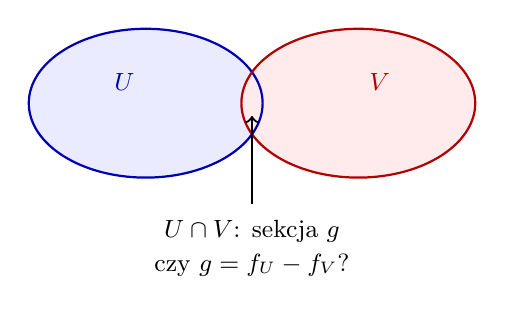
\begin{tikzpicture}[scale=.9,every node/.style={font=\small}]
  \fill[blue!8] (-1.5,0) ellipse (1.65 and 1.05);
  \fill[red!8] (1.5,0) ellipse (1.65 and 1.05);
  \draw[blue!70!black,thick] (-1.5,0) ellipse (1.65 and 1.05);
  \draw[red!70!black,thick] (1.5,0) ellipse (1.65 and 1.05);
  \node[blue!70!black] at (-1.8,.3) {$U$};
  \node[red!70!black] at (1.8,.3) {$V$};
  \draw[->,thick] (0,-1.42)--(0,-.18);
  \node[below,align=center] at (0,-1.52)
     {$U\cap V$: sekcja $g$\\[1pt]czy $g=f_U-f_V$?};
\end{tikzpicture}

{\small Rysunek 4.7. Problem kohomologiczny: lokalnie dane są
sekcje, lecz globalne sklejenie wymaga zgodności na przecięciach.}
\end{center}

\begin{uwaga}[Dlaczego nie wystarczy policzyć dowolnego pokrycia?]
Kompleks Čecha zależy od pokrycia. Dopiero po udowodnieniu
odpowiednich twierdzeń porównawczych można utożsamić jego
kohomologię z kohomologią snopa $H^q(X,\mathcal F)$.
Na schematach rozdzielonych pokrycia afiniczne są do tego
przydatne, gdy $\mathcal F$ jest quasi-koherentny:
wszystkie skończone przecięcia otwartych afinicznych są
afiniczne i wyższe kohomologie na nich znikają.
Nie należy natomiast automatycznie utożsamiać grup
$\check H^q$ z $H^q$ dla dowolnego snopa i dowolnego pokrycia.
\end{uwaga}

\section{Kluczowy rachunek afiniczny: dlaczego lokalizacje sklejają się dokładnie?}
\label{sec:affine-cech-proof}

W geometrii afinicznej sekcje $\widetilde M$ odpowiadają
ułamkom modułu $M$. Udowodnimy dokładność kompleksu
występującego przy pokryciu przez podstawowe otwarte.
Jest to rachunkowy fundament twierdzenia o znikaniu
kohomologii snopów quasi-koherentnych na schematach afinicznych.

\begin{twierdzenie}[Dokładny kompleks lokalizacji]
\label{tw:affine-cech-exact}
Niech $A$ będzie pierścieniem przemiennym z jedynką,
$M$ dowolnym $A$-modułem i $f_0,\ldots,f_r\in A$
takimi, że $(f_0,\ldots,f_r)=A$. Wtedy kompleks
\[
0\longrightarrow M\xrightarrow{\epsilon}
\prod_iM_{f_i}\xrightarrow{d^0}
\prod_{i<j}M_{f_if_j}\xrightarrow{d^1}\cdots
\xrightarrow{d^{r-1}}M_{f_0\cdots f_r}\longrightarrow0
\]
jest dokładny; $\epsilon(m)$ jest rodziną obrazów
$m$ we wszystkich lokalizacjach, a różniczki są
określone wzorem z poprzedniej sekcji.
\end{twierdzenie}
\begin{proof}
Pokażemy najpierw, że dokładność ciągu modułów nad
$A$ można sprawdzić po lokalizacji we wszystkich
ideałach pierwszych. Jeśli $N$ jest niezerowym
$A$-modułem, wybieramy $0\ne n\in N$ i ideał
maksymalny $\mathfrak m$ zawierający właściwy ideał
$\operatorname{Ann}(n)=\{a\in A:an=0\}$.
Wówczas $n/1\ne0$ w $N_{\mathfrak m}$:
gdyby $n/1=0$, pewien $s\notin\mathfrak m$
spełniałby $sn=0$, co przeczy zawieraniu
$\operatorname{Ann}(n)\subseteq\mathfrak m$.
W zastosowaniu do jąder i ilorazów wynika stąd,
że kompleks modułów jest dokładny wtedy i tylko wtedy,
gdy pozostaje dokładny po lokalizacji w każdym
ideale pierwszym (lokalizacja jest funktorem dokładnym;
jak wykazano wcześniej przy konstrukcji lokalizacji).

Ustalmy więc $\mathfrak p\in\Spec A$. Ponieważ
$(f_0,\ldots,f_r)=A$, istnieje indeks $j$ z
$f_j\notin\mathfrak p$. W pierścieniu $A_{\mathfrak p}$
element $f_j$ jest jednostką. Po lokalizacji całego
kompleksu w $\mathfrak p$ wprowadźmy dodatkowe działanie
$h:C^q\to C^{q-1}$, które do składowej indeksowanej
przez $(i_0,\ldots,i_{q-1})$ przypisuje składową
indeksowaną przez $(j,i_0,\ldots,i_{q-1})$ z odpowiednim
znakiem permutacji; jeśli indeks $j$ już występuje,
kładziemy tę składową równą zeru. Odwzorowanie jest
poprawnie określone, ponieważ dołączenie $f_j$
nie zmienia lokalizacji po przejściu do $A_{\mathfrak p}$.
Dla $q=0$ przyjmujemy $h:C^0\to M_{\mathfrak p}$,
$h((m_i))=m_j$.

Bezpośrednio z naprzemiennego wzoru na różniczkę
wynikają tożsamości
$h\epsilon=\operatorname{id}$ na $M_{\mathfrak p}$
oraz $dh+hd=\operatorname{id}$ na każdym $C^q$.
Można je sprawdzić, rozpisując składową o ustalonych
indeksach: składnik otrzymany przez usunięcie
wprowadzonego indeksu $j$ jest wyjściową składową,
a wszystkie inne występują parami z przeciwnymi znakami.
Zatem zlokalizowany kompleks jest ściągalny, a więc
dokładny. Stwierdzona na początku lokalna zasada
dokładności kończy dowód.
\end{proof}

\begin{wniosek}[Znikanie wyższej kohomologii Čecha na pokryciu afinicznym]
Niech $X=\Spec A$, $\mathcal F=\widetilde M$ i
$X=\bigcup_{i=0}^rD(f_i)$. Wtedy
$\check H^q(\{D(f_i)\},\mathcal F)=0$ dla
$q>0$, a $\check H^0\cong M$.
\end{wniosek}
\begin{proof}
Dla każdego wielowskaźnika $I$ zachodzi
$\mathcal F(D(\prod_{i\in I}f_i))=M_{\prod_{i\in I}f_i}$.
Zbiory $D(f_i)$ pokrywają $\Spec A$ dokładnie wtedy,
gdy $(f_0,\ldots,f_r)=A$. Teza jest więc
przeformułowaniem twierdzenia~\ref{tw:affine-cech-exact}.
\end{proof}

\begin{uwaga}[Przejście do rzeczywistej kohomologii snopa]
Wykazaliśmy dokładność \emph{konkretnego} kompleksu
Čecha. Pełne stwierdzenie
$H^q(\Spec A,\widetilde M)=0$ dla $q>0$
uzyskuje się, łącząc rachunek lokalizacji z
porównaniem kohomologii Čecha z kohomologią
snopową na pokryciach acyklicznych. Jest to
\emph{twierdzenie o acykliczności afinicznej};
w dalszych obliczeniach używamy go jawnie,
a nie wyprowadzamy z samego faktu, że pewne sekcje
potrafimy skleić. Jego typowe dowody korzystają
z rezolwent iniektywnych lub z teorii kohomologii
Čecha i rozdrobnienia pokryć.
\end{uwaga}

\begin{przyklad}[Dlaczego funktor sekcji globalnych nie jest prawostronnie dokładny?]
Na $\PP^1_k$ rozważmy ciąg snopów
\[
0\longrightarrow\mathcal O(-2)
\xrightarrow{\,(-X_1,X_0)\,}\mathcal O(-1)^{\oplus2}
\xrightarrow{\,(X_0,X_1)\,}\mathcal O\longrightarrow0.
\]
Mapy są dobrze określone, bo mnożenie przez współrzędną
jednorodną stopnia jeden przenosi $\mathcal O(m)$ w
$\mathcal O(m+1)$. Złożenie wynosi zero.
W otoczeniu $X_0\ne0$ pierwsza współrzędna drugiej
mapy jest lokalnie odwracalna, a jądro jest generowane
przez $(-X_1,X_0)$. Analogicznie na $X_1\ne0$.
Ciąg jest zatem dokładny na źdźbłach, czyli jako
ciąg snopów. Jednak
$H^0(\PP^1,\mathcal O(-1))=0$, podczas gdy
$H^0(\PP^1,\mathcal O)=k$.
Odwzorowanie $H^0(\mathcal O(-1)^{\oplus2})\to
H^0(\mathcal O)$ jest więc zerowe, a nie surjektywne.
Brakujące sekcje są wykrywane przez
$H^1(\PP^1,\mathcal O(-2))\cong k$.
Jest to konkretny powód wprowadzania kohomologii.
\end{przyklad}

\section{Residua na zwartej powierzchni Riemanna}
\label{sec:residue-compact}

W tej sekcji pracujemy nad $\C$ i korzystamy z
analityfikacji gładkiej rzutowej krzywej. Jej
przestrzeń punktów zespolonych jest zwartą
spójną powierzchnią Riemanna $S$. Zastosowanie
zespolonej analizy jednej zmiennej pozwoli
udowodnić globalne twierdzenie o residuach bez
zakładania istnienia globalnej współrzędnej wymiernej.

\begin{definicja}[Residuum meromorficznej formy]
Niech $S$ będzie powierzchnią Riemanna, $P\in S$,
$t$ holomorficzną współrzędną lokalną z $t(P)=0$,
a $\omega$ meromorficzną $1$-formą w otoczeniu $P$.
W zapisie
$\omega=(\sum_{j\ge-N}a_jt^j)\,dt$
definiujemy $\operatorname{Res}_P\omega=a_{-1}$.
Współczynnik ten nie zależy od wyboru współrzędnej.
\end{definicja}
\begin{proof}[Uzasadnienie niezależności współrzędnej]
Dla małego dodatnio zorientowanego okręgu
$\gamma:|t|=\varepsilon$ szereg Laurenta można
całkować wyraz po wyrazie. Wobec tego
$\int_\gamma t^j\,dt=0$ dla $j\ne-1$,
a $\int_\gamma dt/t=2\pi i$. Otrzymujemy wzór
\[
\operatorname{Res}_P\omega=
 \frac1{2\pi i}\int_\gamma\omega.
\]
Dwie lokalne współrzędne prowadzą do małych
okręgów otaczających $P$ i homologicznych w
przekłutym otoczeniu, a $\omega$ jest tam
holomorficzna. Z twierdzenia Cauchy'ego całki
są równe. Tak więc definicja jest wewnętrzna,
a nie zależna od parametryzacji.
\end{proof}

\begin{twierdzenie}[Globalne twierdzenie o sumie residuów]
\label{tw:residue-general}
Niech $S$ będzie zwartą spójną powierzchnią
Riemanna, a $\omega$ meromorficzną $1$-formą na $S$.
Wtedy ma ona tylko skończenie wiele biegunów i
\[
\sum_{P\in S}\operatorname{Res}_P\omega=0.
\]
\end{twierdzenie}
\begin{proof}
Bieguny formy meromorficznej są dyskretne.
Ich zbiór jest domknięty w zwartej przestrzeni $S$,
zatem jest skończony; oznaczmy go $P_1,\ldots,P_s$.
Wybierzmy wokół tych punktów parami rozłączne,
małe domknięte dyski współrzędnych $D_j$,
takie że na każdej krzywej brzegowej $\partial D_j$
forma $\omega$ jest holomorficzna.
Niech $S^\circ=S\setminus\bigcup_j\operatorname{int}D_j$.
Na zwartej rozmaitości z brzegiem $S^\circ$
forma $\omega$ jest holomorficzna, toteż zamknięta:
$\mathrm d\omega=0$. Z twierdzenia Stokesa
otrzymujemy
\[
0=\int_{S^\circ}\mathrm d\omega
 =\int_{\partial S^\circ}\omega
 =-\sum_{j=1}^s\int_{\partial D_j}\omega
 =-2\pi i\sum_{j=1}^s\operatorname{Res}_{P_j}\omega.
\]
Znak minus wynika stąd, że dodatnia orientacja
brzegu powierzchni z \emph{wyciętymi} dyskami
jest przeciwna do dodatniej orientacji okręgów
otaczających bieguny. Podzielenie przez $-2\pi i$
daje tezę.
\end{proof}

\begin{center}
\begin{tikzpicture}[scale=.9,every node/.style={font=\small},>=Stealth]
  \fill[blue!6] (0,0) ellipse (3.05 and 1.65);
  \draw[blue!70!black,thick] (0,0) ellipse (3.05 and 1.65);
  \fill[white] (-1.25,.1) circle (.38);
  \fill[white] (1.25,-.15) circle (.38);
  \draw[red!75!black,thick] (-1.25,.1) circle (.38);
  \draw[red!75!black,thick] (1.25,-.15) circle (.38);
  \fill[red!75!black] (-1.25,.1) circle (1.4pt);
  \fill[red!75!black] (1.25,-.15) circle (1.4pt);
  \node[above] at (-1.25,.53) {$P_1$};
  \node[above] at (1.25,.32) {$P_2$};
  \node at (0,1.08) {$S^\circ$};
  \node[below,align=center] at (0,-1.85)
     {Wycięte dyski mają brzeg przeciwnie zorientowany\\
      do małych dodatnich okręgów wokół biegunów.};
\end{tikzpicture}

{\small Rysunek 4.8. Schemat idei dowodu twierdzenia o sumie residuów.
Rysunek przedstawia powierzchnię \emph{schematycznie}, a nie jako
metrycznie wierne zanurzenie powierzchni Riemanna.}
\end{center}

\begin{wniosek}[Stopień dywizora funkcji wymiernej raz jeszcze]
Jeżeli $S$ jest zwartą spójną powierzchnią
Riemanna, a $f$ jest niezerową funkcją meromorficzną,
to suma rzędów jej zer i biegunów wynosi zero:
$\sum_{P\in S}\operatorname{ord}_P(f)=0$.
\end{wniosek}
\begin{proof}
W pobliżu dowolnego punktu $P$ piszemy
$f=t^mu(t)$, gdzie $m\in\Z$ oraz $u$ jest
holomorficzna i nigdzie nie znika. Zatem
$\mathrm df/f=m\,\mathrm dt/t+\mathrm du/u$.
Drugi składnik jest holomorficzny, a pierwszy
ma residuum $m$. Z twierdzenia~\ref{tw:residue-general}
dla formy $\mathrm df/f$ wynika
$0=\sum_P\operatorname{Res}_P(\mathrm df/f)
=\sum_P\operatorname{ord}_P(f)$.
Ten dowód jest niezależny od wcześniejszego
rachunku charakterystyki Eulera.
\end{proof}

\begin{przyklad}[Krzywa eliptyczna i regularność różniczki]
Niech $E$ będzie gładką zespoloną kubiką
$y^2=x^3+ax+b$ z $4a^3+27b^2\ne0$.
Forma $\omega=\mathrm dx/(2y)$ jest holomorficzna
na całym $E$, mimo że jej zapis wygląda osobliwie
w punktach, gdzie $y=0$. W takim punkcie
$3x^2+a\ne0$ (bo równanie jest bez pierwiastków
wielokrotnych), a różniczkowanie równania daje
$2y\,\mathrm dy=(3x^2+a)\,\mathrm dx$, czyli
$\omega=\mathrm dy/(3x^2+a)$; to wyrażenie jest
regularne. W punkcie w nieskończoności użyjmy
parametrów $u=X/Y$, $v=Z/Y$ z przykładu
\ref{prz:weierstrass-LmO}. Tam $v$ ma rząd $3$
i $u$ jest parametrem lokalnym, więc
$x=u/v$ ma rząd $-2$, a $y=1/v$ rząd $-3$.
Dokładniej $v=u^3(1+O(u^4))$, skąd
$x=u^{-2}(1+O(u^4))$ oraz
$y=u^{-3}(1+O(u^4))$ i
$\omega=(-1+O(u^4))\,\mathrm du$.
Forma nie ma bieguna również w nieskończoności.
W szczególności wszystkie jej residua są zerowe.
\end{przyklad}

\section{Części główne, residua i parowanie dualności}
\label{sec:principal-residue-pairing}

\begin{definicja}[Część główna w punkcie]
Niech $C$ będzie gładką rzutową krzywą nad $\C$,
$P\in C$, a $t$ parametrem lokalnym. Częścią główną
funkcji meromorficznej $f=\sum_{j\ge-N}a_jt^j$
w $P$ nazywamy klasę
$\operatorname{pp}_P(f)=\sum_{j=-N}^{-1}a_jt^j$
modulo funkcje holomorficzne w $P$.
Innymi słowy, jest to element ilorazu
$\mathcal M_P/\mathcal O_{C,P}$, gdzie
$\mathcal M_P$ oznacza kiełki funkcji meromorficznych.
\end{definicja}

\begin{przyklad}[Przeszkoda w wyznaczeniu funkcji o zadanym biegunie]
Na $\PP^1$ zadana część główna $t^{-3}+2t^{-1}$
w punkcie $t=0$ jest realizowana przez globalną
funkcję wymierną $t^{-3}+2t^{-1}$. Na krzywej
eliptycznej $E$ nie da się natomiast zrealizować
części głównej $t^{-1}$ w jednym punkcie $P$ przez
funkcję wymierną bez innych biegunów:
taka funkcja należałaby do $L(P)\setminus L(0)$,
a \ref{tw:ell-poles} daje $L(P)=L(0)=\C$.
Jest to przykład globalnej przeszkody przy
pozornie poprawnych danych lokalnych.
\end{przyklad}

\begin{twierdzenie}[Residua wykrywają konieczny warunek realizacji części głównych]
Niech $C$ będzie gładką rzutową krzywą nad $\C$,
$P_1,\ldots,P_s$ parami różnymi punktami, a $p_j$
częściami głównymi w $P_j$. Jeśli istnieje globalna
funkcja meromorficzna $f$ na $C$ mająca dokładnie
te części główne i bez innych biegunów, to
\[
\sum_{j=1}^{s}\operatorname{Res}_{P_j}
  (p_j\,\omega)=0
\quad\text{dla każdej globalnej holomorficznej
różniczki }\omega\in H^0(C,\Omega^1_C).
\]
\end{twierdzenie}
\begin{proof}
Lokalna różnica $f-p_j$ jest holomorficzna
w $P_j$. Ponieważ $\omega$ jest tam holomorficzna,
formy $f\omega$ i $p_j\omega$ mają takie samo
residuum. W każdym pozostałym punkcie $f\omega$
jest holomorficzna. Sumując residua formy
meromorficznej $f\omega$ i stosując
twierdzenie~\ref{tw:residue-general}, otrzymujemy tezę.
\end{proof}

\begin{przyklad}[Dlaczego prosty biegun na torusie nie istnieje — dowód z residuów]
Na krzywej eliptycznej $E$ forma $\omega=\mathrm dx/(2y)$
nie znika nigdzie: na części afinicznej w punktach
$y\ne0$ jest niezerowa, bo $x$ jest parametrem;
w punktach $y=0$ forma $\mathrm dy/(3x^2+a)$ jest
niezerowa, a w nieskończoności ma współczynnik $-1$
przy $\mathrm du$. Jeśli $f$ miałaby jedyny prosty
biegun w $P$, to w parametrze $t$ mielibyśmy
$f=c_{-1}t^{-1}+O(1)$, $c_{-1}\ne0$, oraz
$\omega=(a_0+O(t))\,\mathrm dt$, $a_0\ne0$.
Stąd $\operatorname{Res}_P(f\omega)=c_{-1}a_0\ne0$.
Wszystkie pozostałe residua $f\omega$ są zerowe,
co przeczy twierdzeniu o ich sumie.
To drugi, niezależny rachunek wyjaśniający lukę
w rzędach biegunów funkcji na krzywej eliptycznej.
\end{przyklad}

\begin{uwaga}[Co dodaje pełna dualność Serre'a?]
Poprzednie twierdzenie daje \emph{warunek konieczny}.
Twierdzenie Mittag--Lefflera dla zwartych powierzchni
Riemanna mówi, że warunek znikania residuów względem
wszystkich globalnych holomorficznych różniczek
jest również wystarczający. W sformułowaniu
kohomologicznym odpowiada to niezdegenerowanemu
parowaniu
$H^1(C,\mathcal O_C)\times H^0(C,\Omega^1_C)\to\C$.
W przeciwieństwie do udowodnionej sumy residuów
część o wystarczalności wymaga dodatkowej teorii:
można ją uzyskać z twierdzenia Dolbeaulta i teorii
harmonicznych form różniczkowych. Poniżej podajemy
konstrukcję parowania oraz precyzyjną rolę tych
narzędzi; nie zastępujemy ich pozornie elementarnym
argumentem.
\end{uwaga}

\begin{stwierdzenie}[Parowanie Čecha i residuów na krzywej zespolonej]
\label{st:cech-res-pairing}
Niech $C$ będzie gładką spójną krzywą rzutową nad $\C$,
$\mathcal L$ holomorficzną wiązką liniową na $C^{\mathrm{an}}$,
a $\omega\in H^0(C^{\mathrm{an}},K_C\otimes\mathcal L^{-1})$.
Wybierzmy punkt $P\in C$, dysk współrzędnych $V$
wokół $P$ oraz $U=C\setminus\{P\}$.
Jeśli $g_{UV}$ jest holomorficzną sekcją $\mathcal L$
na pierścieniu $U\cap V$, to liczba
\[
\langle[g_{UV}],\omega\rangle
 =\frac1{2\pi i}\int_{\gamma}g_{UV}\,\omega,
\]
gdzie $\gamma$ jest małym dodatnim okręgiem wokół $P$,
nie zmienia się po zastąpieniu $g_{UV}$ przez
$g_{UV}+s_U|_{U\cap V}-s_V|_{U\cap V}$,
$s_U\in\mathcal L(U)$, $s_V\in\mathcal L(V)$.
Przy mnożeniu używamy naturalnego parowania
$\mathcal L\otimes (K_C\otimes\mathcal L^{-1})\to K_C$.
\end{stwierdzenie}
\begin{proof}
Po dodaniu $s_V$ całka nie zmieni się, bo
$s_V\omega$ jest holomorficzną formą na całym dysku
$V$; jej całka po $\gamma$ jest zerowa z twierdzenia
Cauchy'ego. Z kolei $s_U\omega$ jest holomorficzną
formą na $U$, czyli na powierzchni zwartej pozbawionej
punktu $P$. Wybierzmy mały dysk $D$ wokół $P$.
Na zwartym $C\setminus\operatorname{int}D$
forma $s_U\omega$ jest zamknięta. Stokes daje
$-\int_{\partial D}s_U\omega=0$, więc także
jej całka po $\gamma$ wynosi zero. Są to dokładnie
dwa rodzaje zmian reprezentanta dopuszczalne
w grupie Čecha. Dlatego parowanie zależy tylko
od klasy $[g_{UV}]$.
\end{proof}

\begin{uwaga}[Dlaczego to jest model ogólnej dualności?]
Zbiór $U=C\setminus\{P\}$ jest niezwartą powierzchnią
Riemanna, a zatem przestrzenią Steina na mocy twierdzenia
Behnkego--Steina. Dysk $V$ i pierścień $U\cap V$
są dziedzinami Steina;
także ich przecięcie jest przestrzenią Steina.
Twierdzenie Cartana B daje znikanie wyższej
kohomologii snopów koherentnych na tych częściach,
a twierdzenie porównawcze Čecha pozwala obliczać
$H^1(C^{\mathrm{an}},\mathcal L)$ z takiego pokrycia.
Twierdzenie Dolbeaulta identyfikuje tę grupę
z klasami $\bar\partial$-zamkniętych $(0,1)$-form
o wartościach w $\mathcal L$ modulo obrazy $\bar\partial$.
Poprzez rozkład jedności reprezentant Čecha
przechodzi w taką formę, a powyższa całka konturowa
zgadza się (z uwzględnieniem normalizacji $2\pi i$)
z całką formy $(1,1)$ po $C$.

W konsekwencji \emph{analityczna dualność Serre'a}
może być dowodzona za pomocą teorii Hodge'a:
harmoniczne $(0,1)$-formy z wartościami w
$\mathcal L$ są antyliniowo dualne do
holomorficznych sekcji $K_C\otimes\mathcal L^{-1}$.
Niezerowa forma harmoniczna ma nieznikającą normę
$L^2$, co zapewnia niezdegenerowaność parowania.
\emph{Twierdzenia Steina, Cartana B, Dolbeaulta i Hodge'a
są tu używane jako jawnie nazwane rezultaty.}
Własność niezależności parowania od reprezentantów
oraz samą globalną sumę residuów udowodniliśmy
natomiast bez ich przywoływania.
\end{uwaga}


\begin{uwaga}[Czego wymaga przejście od analizy do geometrii algebraicznej?]
Niech $C$ będzie gładką rzutową krzywą nad $\C$, a
$\mathcal L$ algebraiczną wiązką liniową. Jej
\emph{analityfikacja} $\mathcal L^{\mathrm{an}}$ jest
wiązką holomorficzną na zwartej powierzchni Riemanna
$C^{\mathrm{an}}$ (podstawowa topologia to zwykła
topologia zespolona, a nie topologia Zariskiego).
\emph{Twierdzenie porównawcze GAGA Serre'a} daje
naturalne izomorfizmy
$H^i(C,\mathcal L)\cong
H^i(C^{\mathrm{an}},\mathcal L^{\mathrm{an}})$
dla wszystkich $i\ge0$. Nie dowodzimy tu twierdzenia
GAGA. Jest ono koniecznym, \emph{zewnętrznym}
mostem między poniższym analitycznym dowodem dualności
a jej użyciem dla algebraicznych snopów na krzywych
zespolonych. Nad dowolnym algebraicznie domkniętym
ciałem (również dodatniej charakterystyki)
algebraiczna dualność Serre'a jest osobnym twierdzeniem;
nie wynika z przedstawionych metod Hodge'a.
\end{uwaga}

\begin{twierdzenie}[Dlaczego teoria Hodge'a daje niezdegenerowanie]
\label{tw:serre-hodge-dependent}
Niech $C$ będzie zwartą powierzchnią Riemanna,
a $\mathcal L$ holomorficzną wiązką liniową.
Przyjmijmy \emph{twierdzenie Dolbeaulta} oraz
\emph{twierdzenie Hodge'a dla operatora $\bar\partial$}:
każda klasa $H^1(C,\mathcal L)$ ma dokładnie jednego
reprezentanta harmonicznego w wybranych metrykach
hermitowskich. Wówczas parowanie
\[
H^1(C,\mathcal L)\times
H^0(C,K_C\otimes\mathcal L^{-1})\longrightarrow\C,
\qquad([\alpha],\omega)\longmapsto
\int_C\alpha\wedge\omega
\]
jest niezdegenerowane.
\end{twierdzenie}
\begin{proof}[Dowód oparty na jawnie przyjętych twierdzeniach analitycznych]
Wybierzmy hermitowską metrykę na $\mathcal L$ i metrykę
na $C$. Niech $0\ne[\alpha]\in H^1(C,\mathcal L)$;
z twierdzenia Hodge'a ma on niezerowego harmonicznego
reprezentanta $\alpha$. W lokalnej współrzędnej $z$
i holomorficznej ramie $e$ wiązki piszemy
$\alpha=a(z)\,\mathrm d\bar z\otimes e$ i
$\lambda(z)=\lVert e\rVert^2>0$.
Harmoniczność oznacza $\bar\partial\alpha=0$ oraz
$\bar\partial^*\alpha=0$. Pierwsza równość jest
automatyczna w zespolonym wymiarze jeden.
Druga, po całkowaniu przez części w lokalnym iloczynie
skalarnym, jest równoważna równaniu
$\partial_z(\lambda a)=0$ (ewentualne dodatnie czynniki
pochodzące od metryki na $C$ nie wpływają na jądro).
Zatem funkcja $\lambda\overline a$ jest holomorficzna.

Formuły $\omega=\lambda\overline a\,\mathrm dz\otimes e^{-1}$
na lokalnych mapach tworzą globalną holomorficzną
sekcję $K_C\otimes\mathcal L^{-1}$. Sprawdźmy zgodność
przy zmianie ramy: jeśli $e'=g e$, to
$a'=a/g$ i $\lambda'=|g|^2\lambda$,
więc $\lambda'\overline{a'}(e')^{-1}
=\lambda\overline a\,e^{-1}$. Zgodność przy zmianie
współrzędnej wynika z przekształcania
$\mathrm d\bar z$ i $\mathrm dz$.
Wybierając tę sekcję w parowaniu, otrzymujemy
w lokalnych współrzędnych formę
$\alpha\wedge\omega=
\lambda|a|^2\,\mathrm d\bar z\wedge\mathrm dz$.
Jej całka różni się od dodatniej normy $L^2$ formy
$\alpha$ tylko stałym niezerowym czynnikiem,
więc nie jest zerowa. Pokazaliśmy niezdegenerowanie
względem pierwszego argumentu.

W odwrotną stronę, dla holomorficznej niezerowej
sekcji $\omega=b(z)\,\mathrm dz\otimes e^{-1}$
konstruujemy harmoniczną formę
$\alpha=\lambda^{-1}\overline b\,\mathrm d\bar z\otimes e$.
Równanie $\partial_z(\lambda a)=0$ zachodzi, ponieważ
$\overline b$ jest antyholomorficzna. Ta forma nie
jest zerowa; dzięki twierdzeniu Hodge'a reprezentuje
niezerową klasę. Jej parowanie z $\omega$ jest
niezerową wielokrotnością całki z $|b|^2/\lambda$.
To kończy dowód względnej niezdegenerowaności.

Dowód jest \emph{kompletny po przyjęciu dwóch
wyraźnie sformułowanych twierdzeń analitycznych}.
Nie jest niezależnym dowodem twierdzeń Dolbeaulta
ani Hodge'a; te wymagają teorii eliptycznych
operatorów różniczkowych na zwartych rozmaitościach.
\end{proof}

\begin{przyklad}[Trzy różne typy wiedzy o dualności]
Na $\PP^1$ dysponujemy \emph{pełnym algebraicznym}
dowodem przez bazy Laurenta
(twierdzenie~\ref{tw:serre-p1-explicit}).
Na dowolnej zwartej powierzchni Riemanna
mamy \emph{pełny dowód} globalnego twierdzenia
o sumie residuów (twierdzenie~\ref{tw:residue-general})
oraz bezpośrednią konstrukcję dobrze określonego
parowania konturowego. Niezdegenerowaność
tego parowania dla dowolnej krzywej jest
natomiast \emph{konsekwencją ogólnej dualności},
której fundamenty analityczne zostały powyżej
nazwane, lecz nie udowodnione od podstaw.
Rozróżnienie tych trzech poziomów zapobiega
błędnemu przekonaniu, że lokalny rachunek
residuum automatycznie stanowi dowód całej
dualności Serre'a.
\end{przyklad}


\section{Twierdzenie Mittag--Lefflera: od lokalnych biegunów do funkcji globalnej}
\label{sec:mittag-residue}

Możemy teraz domknąć ideę, od której zaczęła się
kohomologia krzywych. Dane lokalne mogą być zgodne
z definicją funkcji meromorficznej, a jednak nie
pochodzić od \emph{jednej} funkcji na całej krzywej.
Warunki residuowe opisują dokładnie tę przeszkodę.

\begin{definicja}[Snop części głównych ograniczonych dywizorem]
Niech $C$ będzie gładką rzutową krzywą nad $\C$,
$D=\sum_{j=1}^sm_jP_j$ efektywnym dywizorem,
gdzie $m_j\ge1$, a punkty $P_j$ są parami różne.
Oznaczmy przez $\mathcal P_D$ ilorazowy snop
$\mathcal O_C(D)/\mathcal O_C$.
W punkcie $P_j$ wybierzmy parametr $t_j$.
Wtedy $(\mathcal P_D)_{P_j}$ jest przestrzenią
wektorową nad $\C$ o bazie klas
$t_j^{-m_j},\ldots,t_j^{-1}$; poza nośnikiem $D$
źdźbła tego snopa są zerowe. Zatem
\[
 H^0(C,\mathcal P_D)\cong
 \bigoplus_{j=1}^s
 \operatorname{span}_{\C}
 \{t_j^{-m_j},\ldots,t_j^{-1}\}.
\]
To, że podana rodzina istotnie stanowi bazę,
wynika z faktu, że w dyskretnym pierścieniu
wartościowania $\mathcal O_{C,P_j}$ iloraz
$t_j^{-m_j}\mathcal O_{C,P_j}/\mathcal O_{C,P_j}$
ma dokładnie te $m_j$ klasy jednomianów.
\end{definicja}

\begin{twierdzenie}[Mittag--Leffler na gładkiej krzywej zespolonej]
\label{tw:mittag-curve}
Niech $C$ będzie gładką, spójną, rzutową krzywą
nad $\C$, $P_1,\ldots,P_s$ parami różnymi punktami,
a $p_j=\sum_{r=1}^{m_j}a_{jr}t_j^{-r}$
zadanymi częściami głównymi w wybranych parametrach
lokalnych $t_j$ przy $P_j$. Istnieje globalna
funkcja meromorficzna $f$ na $C$, której części
główne są równe $p_j$, i która nie ma innych
biegunów, wtedy i tylko wtedy, gdy
\[
  \sum_{j=1}^{s}\operatorname{Res}_{P_j}
       (p_j\,\omega)=0
  \qquad\text{dla każdej }\omega\in H^0(C,K_C).
\]
Dowód wykorzystuje analityczną dualność Serre'a
uzyskaną z twierdzeń Dolbeaulta i Hodge'a.
\end{twierdzenie}
\begin{proof}
Konieczność została udowodniona w poprzedniej
sekcji za pomocą globalnego twierdzenia o residuach.
Przeprowadźmy dokładnie dowód wystarczalności.

Niech $D=\sum_jm_jP_j$. Włączenie stałych warunków
na brak biegunów w warunki dopuszczające bieguny
rzędów nie większych niż $m_j$ prowadzi do krótkiego
ciągu dokładnego snopów
\[
 0\longrightarrow\mathcal O_C
 \longrightarrow\mathcal O_C(D)
 \longrightarrow\mathcal P_D\longrightarrow0.
\]
Jego dokładność wynika z lokalnych wzorów
$\mathcal O_{C,P_j}\subseteq
 t_j^{-m_j}\mathcal O_{C,P_j}$ oraz identyczności
tych źdźbeł poza punktami $P_j$.
Z długiego ciągu dokładnego kohomologii otrzymujemy
fragment
\[
 H^0(C,\mathcal O_C(D))\xrightarrow{\ q\ }
 H^0(C,\mathcal P_D)\xrightarrow{\ \partial\ }
 H^1(C,\mathcal O_C).
\]
Odwzorowanie $q$ przypisuje funkcji jej części główne.
Z dokładności wynika, że dana rodzina
$p=(p_1,\ldots,p_s)$ pochodzi od globalnej funkcji
meromorficznej z dopuszczonymi biegunami dokładnie wtedy,
gdy $\partial p=0$.

Pozostaje wyjaśnić, jak rozpoznać zerowość tej klasy.
Wybierzmy dla każdego $P_j$ mały dysk $V_j$, przy czym dyski są parami rozłączne, i weźmy
$U=C\setminus\{P_1,\ldots,P_s\}$. Na każdym
$V_j$ wybieramy meromorficzną funkcję $p_j$ realizującą
zadane części główne; na $U$ wybieramy lokalne podniesienie
równe zeru. Różnice podniesień na pierścieniach
$U\cap V_j$ tworzą $1$-kocykl reprezentujący
$\partial p$. Przy konwencji
$\partial p$ reprezentowanej przez $p_j|_{U\cap V_j}$,
parowanie konturowe z globalną holomorficzną różniczką
$\omega$ jest równe
\[
  \langle\partial p,\omega\rangle
  =\sum_{j=1}^s\frac1{2\pi i}
        \int_{\partial D_j}p_j\,\omega
  =\sum_{j=1}^s\operatorname{Res}_{P_j}(p_j\omega).
\]
Jeśli w definicji różniczki Čecha wybiera się
przeciwną konwencję znaku, obie strony zmieniają
znak, co nie wpływa na kryterium znikania.
Równość jest przypadkiem zgodności parowania
Čecha i residuów wykazanej przy
stwierdzeniu~\ref{st:cech-res-pairing}.

Z założenia wszystkie powyższe liczby są zerowe.
Niezdegenerowanie dualności Serre'a
(twierdzenie~\ref{tw:serre-hodge-dependent}) daje
$\partial p=0$. Z dokładności ciągu istnieje
$f\in H^0(C,\mathcal O_C(D))$ takie, że
$q(f)=p$. Sekcja ta jest szukaną funkcją
meromorficzną. To kończy dowód.
\end{proof}

\begin{przyklad}[Sfera i torus: dwa odmienne wyniki dla prostego bieguna]
Na $\PP^1(\C)$ nie ma niezerowych holomorficznych
różniczek, bo $K_{\PP^1}\cong\mathcal O(-2)$.
Warunek z twierdzenia~\ref{tw:mittag-curve}
jest wobec tego pusty: każdą skończoną kolekcję
części głównych funkcji można zrealizować
przez globalną funkcję wymierną.

Na krzywej eliptycznej $E$ istnieje natomiast
niezerowa holomorficzna forma $\omega$ bez zer.
Dla jednej zadanej części głównej $t^{-1}$ w punkcie
$P$ residuum $(t^{-1}\omega)$ jest niezerowe,
więc takiej funkcji nie ma. Dla dwóch punktów
$P,Q$ i części głównych
$a\,t_P^{-1}$ oraz $b\,t_Q^{-1}$
warunek przyjmuje postać
$a\,\omega_P(\partial/\partial t_P)
+b\,\omega_Q(\partial/\partial t_Q)=0$.
Jest to \emph{jedno} równanie liniowe, bo
$\dim H^0(E,K_E)=1$. Kiedy jest spełnione,
możemy wybrać globalną funkcję meromorficzną
z tymi dwiema zadanymi częściami głównymi.
\end{przyklad}

\section{Podsumowanie zależności i wskazówki do dalszej nauki}
\label{sec:summary-four}

Prześledźmy najważniejszy łańcuch pojęć. Lokalizacja
przekształca pierścień globalnych wielomianów
w pierścień funkcji regularnych przy wybranym
punkcie. W przypadku gładkiej krzywej ten lokalny
pierścień ma \emph{jeden parametr} i jest DVR;
dzięki temu możemy bez niejednoznaczności mierzyć
rzędy zer i biegunów. Dywizor łączy te lokalne
liczby w jeden obiekt globalny. Snop
$\mathcal O_C(D)$ tłumaczy warunki na zera i bieguny
na warunki o sekcjach, a kohomologia mierzy
deficyt możliwości sklejania tych sekcji.
Riemann--Roch zamienia tę informację na wzór
numeryczny: stopień dywizora i rodzaj krzywej
określają różnicę dwóch wymiarów.

\begin{center}
\begin{tikzpicture}[node distance=8mm,>=Stealth,
  every node/.style={font=\small},
  summaryblock/.style={draw,rounded corners,align=center,text width=7.5cm,
  inner sep=5pt}]
\node[summaryblock] (a) {Pierścień globalny $A$ i lokalizacja $A_{\mathfrak p}$};
\node[summaryblock,below=of a] (b) {Pierścień lokalny DVR $\to$ rzędy $\operatorname{ord}_P$};
\node[summaryblock,below=of b] (c) {Dywizory $D$ i snopy odwracalne $\mathcal O_C(D)$};
\node[summaryblock,below=of c] (d) {Kohomologia $H^0,H^1$ i dualność Serre'a};
\node[summaryblock,below=of d] (e) {Riemann--Roch, rodzaj, krzywe eliptyczne};
\draw[->,thick] (a)--(b); \draw[->,thick] (b)--(c);
\draw[->,thick] (c)--(d); \draw[->,thick] (d)--(e);
\end{tikzpicture}

{\small Rysunek 4.9. Zależności między narzędziami algebry przemiennej, snopami i geometrią krzywych.}\par
\end{center}

Po rozszerzeniu udowodniliśmy już bezpośrednio dokładność
kompleksu Čecha dla podstawowych pokryć afinicznych,
globalną sumę residuów na zwartej powierzchni Riemanna
oraz dobrze określoność parowania residuowego.
Jawnie oddzielamy od nich użyte głębsze rezultaty:
porównanie kohomologii Čecha z kohomologią snopów,
acykliczność afiniczną w pełnej ogólności, skończoność
kohomologii koherentnej oraz twierdzenia Dolbeaulta
i Hodge'a. Teoria dualności Serre'a została rozwinięta
do konstrukcji parowania i do dowodu jego
niezdegenerowania \emph{przy przyjęciu} dwóch
ostatnich twierdzeń, bez sugerowania, że są one elementarne.

% Źródła referencyjne (nie zastępują dowodów w tekście):
% The Stacks Project, Tags 0C4S, 0A22, 0B5B.
% R. Vakil, The Rising Sea: Foundations of Algebraic Geometry.

% =============================================================
% DODATEK DO ROZDZIALU 4: RESIDUA WIELU ZMIENNYCH
% Wprowadzany po podsumowaniu dotychczasowego rozdzialu 4.
% =============================================================
\section{Residua wielowymiarowe: od całek Cauchy'ego do geometrii przecięć}
\label{sec:ga4-residua-wielo}

\subsection{Dlaczego nie wystarcza residuum jednej zmiennej?}

W jednej zmiennej meromorficzna forma $h(z)\,\mathrm dz/f(z)$
ma izolowane bieguny i możemy całkować po małej okrężnej krzywej.
W $\C^n$ dla $n\ge2$ pojedyncze równanie $f=0$ opisuje na ogół
hiperpowierzchnię, a nie zbiór punktów. W szczególności funkcja
$1/f$ nie ma izolowanego bieguna w sensie jednej zmiennej.
Aby otrzymać \emph{liczbę} z lokalnego całkowania $n$-formy,
rozpatrzymy $n$ funkcji $f_1,\ldots,f_n$ o izolowanym wspólnym zerze.
Inna konstrukcja, \emph{residuum Poincarégo}, będzie przypisywać
formę różniczkową gładkiej hiperpowierzchni $f=0$.
Te dwie konstrukcje pełnią różne role.

\begin{uwaga}[Dwie różne dziedziny całkowania]
W $\C^2$ okrąg $S^1$ ma wymiar rzeczywisty $1$, sfera
$S^3$ ma wymiar $3$, natomiast powierzchnia całkowania
residuum Grothendiecka ma wymiar rzeczywisty $2$:
typowo jest torusem $S^1\times S^1$.
Nie należy bez wyjaśnienia zastępować tego torusa małą sferą $S^3$.
\end{uwaga}

\subsection{Wielowymiarowy wzór Cauchy'ego}
\label{subsec:ga4-cauchy-product}

\begin{twierdzenie}[Wzór Cauchy'ego na polidysku]
\label{tw:ga4-polydisc-cauchy}
Niech $a=(a_1,\ldots,a_n)\in\C^n$, $r_j>0$, a $h$ będzie
holomorficzna w otoczeniu domkniętego polidysku
$\overline P(a,r)=\{z\in\C^n:|z_j-a_j|\le r_j,\ 1\le j\le n\}$.
Wówczas dla $z\in P(a,r)$ zachodzi
\[
 h(z)=\frac{1}{(2\pi i)^n}
 \int_{|\zeta_1-a_1|=r_1}\!\cdots
 \int_{|\zeta_n-a_n|=r_n}
 \frac{h(\zeta_1,\ldots,\zeta_n)}
 {\prod_{j=1}^n(\zeta_j-z_j)}
 \,\mathrm d\zeta_n\cdots\mathrm d\zeta_1.
\]
Każdą okręgową krzywą całkujemy przeciwnie do ruchu wskazówek
zegara; porządek całkowań został tu jawnie ustalony.
\end{twierdzenie}
\begin{proof}
Traktujemy $\zeta_2,\ldots,\zeta_n$ jako ustalone parametry.
Jednowymiarowy wzór Cauchy'ego względem $\zeta_1$ zastępuje
pierwszą całkę wartością funkcji przy $\zeta_1=z_1$.
Pozostała funkcja jest holomorficzna w następnej zmiennej,
więc ponownie stosujemy wzór Cauchy'ego. Po $n$ krokach
otrzymujemy $h(z_1,\ldots,z_n)$.
Wszystkie całki są całkami funkcji ciągłych po zwartych torusach,
co uzasadnia zamianę kolejności ich obliczania w tej właśnie
sytuacji produktu niezależnych okręgów.
\end{proof}

\begin{wniosek}[Wzór na współczynnik Taylora]
\label{wn:ga4-monomial-res}
Niech $m_1,\ldots,m_n\ge1$ będą liczbami całkowitymi,
a $h$ funkcją holomorficzną w otoczeniu domkniętego
polidysku $\{z\in\C^n:|z_j|\le r_j,\ 1\le j\le n\}$
dla ustalonych $r_1,\ldots,r_n>0$. Wówczas
\[
\frac{1}{(2\pi i)^n}\int_{|z_1|=r_1}\!\cdots
\int_{|z_n|=r_n}
\frac{h(z)\,\mathrm dz_n\cdots\mathrm dz_1}
{z_1^{m_1}\cdots z_n^{m_n}}
=\frac{\partial_1^{m_1-1}\cdots\partial_n^{m_n-1}h(0)}
{(m_1-1)!\cdots(m_n-1)!}.
\]
W szczególności całka odczytuje współczynnik przy
$z_1^{m_1-1}\cdots z_n^{m_n-1}$ w szeregu Taylora funkcji $h$.
\end{wniosek}
\begin{proof}
Z jednowymiarowego wzoru Cauchy'ego dla pochodnych
obliczamy najpierw całkę po okręgu w pierwszej zmiennej.
Następnie powtarzamy ten rachunek w pozostałych zmiennych.
Wynik jest podaną pochodną mieszaną podzieloną przez
iloczyn silni. Kolejność różniczkowania funkcji
holomorficznej nie zmienia wyniku.
\end{proof}

\begin{przyklad}[Residuowe odczytywanie współczynników]
W $\C^2$ rozważmy $h(z,w)=e^{z+w}$.
Wielomian Taylora pokazuje, że współczynnik $zw^2$ wynosi $1/2$.
Dlatego
\[
\frac{1}{(2\pi i)^2}\int_{|z|=r}\int_{|w|=s}
\frac{e^{z+w}}{z^2w^3}\,\mathrm dw\,\mathrm dz=\frac12.
\]
Natomiast całka z $1/(z^2w^3)$ wynosi zero. Sam fakt,
że mianownik ma biegun w każdej zmiennej, nie wystarcza,
aby residuum było niezerowe.
\end{przyklad}

\begin{center}
\begin{tikzpicture}[>=Stealth,scale=0.95]
 \draw[->,gray!70] (-4.8,0)--(-2.25,0) node[right,font=\scriptsize] {$\Re z$};
 \draw[->,gray!70] (-3.5,-1.15)--(-3.5,1.25) node[above,font=\scriptsize] {$\Im z$};
 \draw[thick,blue!70!black] (-3.5,0) circle (0.72);
 \node[below,font=\footnotesize] at (-3.5,-1.35) {$|z|=r$};
 \draw[->,gray!70] (0.0,0)--(2.5,0) node[right,font=\scriptsize] {$\Re w$};
 \draw[->,gray!70] (1.2,-1.15)--(1.2,1.25) node[above,font=\scriptsize] {$\Im w$};
 \draw[thick,teal!70!black] (1.2,0) circle (0.72);
 \node[below,font=\footnotesize] at (1.2,-1.35) {$|w|=s$};
 \node[draw,rounded corners,align=center,font=\footnotesize,
       text width=9.0cm,minimum height=0.72cm] at (-1.15,-2.47)
 {$\Gamma=\{(z,w):|z|=r,\ |w|=s\}\cong S^1\times S^1$
 \quad (torus o wymiarze rzeczywistym $2$)};
\end{tikzpicture}

{\small Rysunek 4.10. Torus całkowania jako produkt dwóch dodatnio
zorientowanych okręgów. Nie jest on sferą trójwymiarową.}\par
\end{center}

\subsection{Residuum Grothendiecka w izolowanym wspólnym zerze}
\label{subsec:ga4-groth-res}

\begin{definicja}[Residuum lokalne Grothendiecka]
\label{def:ga4-groth-res}
Niech $U\subseteq\C^n$ będzie otwarte, $a\in U$, a funkcje
$f_1,\ldots,f_n,h\in\mathcal O(U)$ takie, że $a$ jest
\emph{izolowanym} punktem zbioru
$\{z\in U:f_1(z)=\cdots=f_n(z)=0\}$.
Wybierzmy dostatecznie małe otoczenie $V$ punktu $a$,
nie zawierające innego wspólnego zera, oraz dostatecznie małe regularne
wartości dodatnie $\varepsilon_j$ funkcji $|f_j|$,
tak aby rzeczywisty cykl
\[
\Gamma_\varepsilon=\{z\in V:|f_1(z)|=\varepsilon_1,\ldots,
|f_n(z)|=\varepsilon_n\}
\]
był zawarty w tym otoczeniu.
Orientację wyznacza dodatniość formy
$\mathrm d\arg f_1\wedge\cdots\wedge\mathrm d\arg f_n$.
Definiujemy
\[
\operatorname{Res}_a\!\left[\frac{h\,\mathrm dz_1\wedge\cdots
\wedge\mathrm dz_n}{f_1\cdots f_n}\right]
=\frac1{(2\pi i)^n}\int_{\Gamma_\varepsilon}
\frac{h(z)\,\mathrm dz_1\wedge\cdots\wedge\mathrm dz_n}
{f_1(z)\cdots f_n(z)}.
\]
Wybór otoczenia i dostatecznie małych $\varepsilon_j$
nie zmienia wartości całki; to własność dobrze określonego
lokalnego cyklu residuowego.
\end{definicja}

\begin{uwaga}[Co jest twierdzeniem, a co definicją?]
Istnienie odpowiedniego małego cyklu i niezależność jego
klasy homologii od dostatecznie małych parametrów wynika
z lokalnej teorii skończonych odwzorowań holomorficznych
lub z konstrukcji cyklu Leraya. To jest odrębny wynik
analityczny, przyjmowany tutaj jawnie; w przykładach
regularnych sprowadza się on do zmiany współrzędnych,
a w przypadku jednomianowym do torusa produktowego.
Zapis $\operatorname{Res}_a$ zawsze odnosi się do \emph{uporządkowanej}
listy $(f_1,\ldots,f_n)$, nie tylko do ideału, który generują.
\end{uwaga}

\begin{twierdzenie}[Proste wspólne zero: wzór jakobianowy]
\label{tw:ga4-jac-res}
Niech $f_1,\ldots,f_n,h$ będą holomorficzne w otoczeniu
$a\in\C^n$, spełniają $f_j(a)=0$ dla każdego $j$, a
\[
J_f(a)=\det\left(\frac{\partial f_i}{\partial z_j}(a)
\right)_{1\le i,j\le n}\ne0.
\]
Wówczas $a$ jest izolowanym wspólnym zerem i
\[
\operatorname{Res}_a\!\left[
\frac{h\,\mathrm dz_1\wedge\cdots\wedge\mathrm dz_n}
{f_1\cdots f_n}\right]=\frac{h(a)}{J_f(a)}.
\]
\end{twierdzenie}
\begin{proof}
Holomorficzne twierdzenie o odwzorowaniu odwrotnym
mówi, że $u=f(z)$ są współrzędnymi holomorficznymi
w otoczeniu $a$. Ponieważ
$\mathrm du_1\wedge\cdots\wedge\mathrm du_n
=J_f(z)\,\mathrm dz_1\wedge\cdots\wedge\mathrm dz_n$,
podcałkowa forma przyjmuje postać
$\bigl(h(z(u))/J_f(z(u))\bigr)\mathrm du_1\wedge\cdots
\wedge\mathrm du_n/(u_1\cdots u_n)$.
Cykl $\Gamma_\varepsilon$ przechodzi na standardowy torus
$|u_j|=\varepsilon_j$, z jego dodatnią orientacją.
Wielowymiarowy wzór Cauchy'ego daje wartość
$h(a)/J_f(a)$.
\end{proof}

\begin{przyklad}[Jakobian i znak residuum]
Weźmy $f_1(z,w)=z+w$, $f_2(z,w)=z-w$ i $h\equiv1$.
Wspólne zero to $(0,0)$, a jakobian ma wyznacznik
$\det\begin{pmatrix}1&1\\1&-1\end{pmatrix}=-2$.
Zatem
$\operatorname{Res}_{(0,0)}[\mathrm dz\wedge\mathrm dw/
((z+w)(z-w))]=-1/2$.
Po zamianie kolejności mianowników otrzymamy $+1/2$.
Nie jest to błąd rachunkowy: orientacja cyklu zależy od
kolejności funkcji definiujących przecięcie.
\end{przyklad}

\subsection{Zera wielokrotne i lokalna algebra}
\label{subsec:ga4-res-multiple}

Nie wolno stosować wzoru $h(a)/J_f(a)$, gdy $J_f(a)=0$.
Residuum może jednak nadal istnieć i być łatwe do obliczenia.

\begin{twierdzenie}[Wzór jednomianowy dla residuum]
\label{tw:ga4-res-monomial}
Niech $m_1,\ldots,m_n\ge1$, a $h$ będzie holomorficzna
w otoczeniu zera w $\C^n$. Wtedy
\[
\operatorname{Res}_0\!\left[
\frac{h(z)\,\mathrm dz_1\wedge\cdots\wedge\mathrm dz_n}
{z_1^{m_1}\cdots z_n^{m_n}}\right]
=\frac{\partial_1^{m_1-1}\cdots\partial_n^{m_n-1}h(0)}
{\prod_{j=1}^n(m_j-1)!}.
\]
\end{twierdzenie}
\begin{proof}
Cykl $|z_j^{m_j}|=\varepsilon_j$ jest torusem produktowym
$|z_j|=\varepsilon_j^{1/m_j}$; jego orientacja jest
zgodna ze standardową, ponieważ każda funkcja
$z_j\mapsto z_j^{m_j}$ zachowuje orientację okręgu.
Stosujemy wniosek~\ref{wn:ga4-monomial-res}.
\end{proof}

\begin{przyklad}[Jakobian znika, lecz residuum nie]
Dla $f_1=z^2$ i $f_2=w^2$ mamy $J_f(0,0)=0$.
Mimo to $\operatorname{Res}_0[zw\,\mathrm dz\wedge\mathrm dw/
(z^2w^2)]=1$ oraz
$\operatorname{Res}_0[\mathrm dz\wedge\mathrm dw/(z^2w^2)]=0$.
Lokalny iloraz $\C\{z,w\}/(z^2,w^2)$ ma bazę
$1,z,w,zw$, więc ma wymiar $4$ nad $\C$.
Wartość residuum nie jest po prostu tą długością:
jest funkcjonałem liniowym zależnym od licznika $h$.
\end{przyklad}

\begin{twierdzenie}[Twierdzenie o transformacji residuum — wynik zewnętrzny]
\label{tw:ga4-res-transform}
Niech $a$ będzie izolowanym wspólnym zerem
$f=(f_1,\ldots,f_n)$, gdzie $f_j$ są holomorficzne
w otoczeniu $a$. Niech $A=(a_{ij})$ będzie macierzą
funkcji holomorficznych, a $g_i=\sum_{j=1}^n a_{ij}f_j$.
Załóżmy, że $a$ jest również izolowanym wspólnym zerem
$g=(g_1,\ldots,g_n)$. Wówczas dla każdej holomorficznej
funkcji $h$ zachodzi
\[
\operatorname{Res}_a\!\left[
\frac{h\,\mathrm dz_1\wedge\cdots\wedge\mathrm dz_n}
{f_1\cdots f_n}\right]
=\operatorname{Res}_a\!\left[
\frac{h\det A\,\mathrm dz_1\wedge\cdots\wedge\mathrm dz_n}
{g_1\cdots g_n}\right].
\]
\end{twierdzenie}

\begin{uwaga}[Dlaczego trzeba uważać na kierunek wzoru?]
Jeżeli $g=Af$, to po \emph{prawej} stronie pojawia się
$\det A$ i mianowniki $g_i$. Nie należy bez sprawdzenia
przenosić wyznacznika na lewą stronę.
Dla $n=1$, $f=z$, $g=z^2=zf$ wzór daje
$\operatorname{Res}_0[h\,\mathrm dz/z]
=\operatorname{Res}_0[hz\,\mathrm dz/z^2]=h(0)$.
Ogólny dowód prawa transformacji korzysta z lokalnych
własności cyklu Grothendiecka (równoważnie z lokalnej
dualności); nie zastępujemy go nieuprawnioną zmianą
zmiennych, gdy $\det A(a)=0$.
\end{uwaga}

\begin{przyklad}[Nietrywialne przecięcie zdegenerowane]
\label{prz:ga4-res-degenerate}
Weźmy $f_1=z^2$ oraz $f_2=w^2+z^3$ w otoczeniu zera.
Wspólne zero jest izolowane, a jakobian $J_f(0)=0$.
Niech $g_1=z^2$ i $g_2=w^2=f_2-zf_1$. Wtedy
\[
\begin{pmatrix}g_1\\g_2\end{pmatrix}
=\begin{pmatrix}1&0\\-z&1\end{pmatrix}
\begin{pmatrix}f_1\\f_2\end{pmatrix},\qquad \det A=1.
\]
Wzór transformacji sprowadza zadanie do współczynnika
przy $zw$ w rozwinięciu licznika $h$:
\[
\operatorname{Res}_0\!\left[
\frac{h(z,w)\,\mathrm dz\wedge\mathrm dw}
{z^2(w^2+z^3)}\right]
=\partial_z\partial_w h(0,0).
\]
Dla $h=1$, $h=zw$ i $h=(z+w)^2$ otrzymujemy
odpowiednio $0$, $1$ i $2$.
Przy tym lokalny pierścień
$\C\{z,w\}/(z^2,w^2+z^3)$ jest izomorficzny z
$\C\{z,w\}/(z^2,w^2)$, z bazą $1,z,w,zw$.
Tak widzimy jednocześnie krotność przecięcia równą $4$
i subtelniejsze informacje zachowywane przez residuum.
\end{przyklad}

\begin{stwierdzenie}[Anulowanie ideału w liczniku]
\label{st:ga4-res-annihilates}
Jeżeli $a$ jest izolowanym wspólnym zerem funkcji
$f_1,\ldots,f_n\in\mathcal O(U)$, a
$h\in(f_1,\ldots,f_n)\mathcal O_{U,a}$, to
\[
\operatorname{Res}_a\!\left[
\frac{h\,\mathrm dz_1\wedge\cdots\wedge\mathrm dz_n}
{f_1\cdots f_n}\right]=0.
\]
\end{stwierdzenie}
\begin{proof}
Możemy przesunąć $a$ do zera. Ponieważ wspólne zero
jest izolowane, lokalny analityczny Nullstellensatz daje
$\sqrt{(f_1,\ldots,f_n)}=(z_1,\ldots,z_n)$,
a zatem dla pewnych $N_i\ge1$ funkcje $g_i=z_i^{N_i}$
należą do ideału $(f_1,\ldots,f_n)$.
Wybierzmy macierz holomorficzną $A$ taką, że $g=Af$.
Z prawa transformacji~\ref{tw:ga4-res-transform} mamy
$\operatorname{Res}_0(h;f)=\operatorname{Res}_0(h\det A;g)$.
Jeśli $h=\sum_j b_jf_j$, to tożsamość macierzowa
$\operatorname{adj}(A)A=(\det A)I$ pokazuje, że
$(\det A)f_j$ jest kombinacją funkcji $g_i$.
Stąd $h\det A\in(g_1,\ldots,g_n)$.
W zapisie $g_i=z_i^{N_i}$ każdy składnik licznika
jest podzielny przez odpowiednie $z_i^{N_i}$,
więc wzór Cauchy'ego na współczynniki daje residuum zero.
Jawnymi przesłankami tego dowodu są lokalny analityczny
Nullstellensatz i twierdzenie o transformacji.
\end{proof}

\begin{uwaga}[Dalsza lokalna dualność]
Dla izolowanego przecięcia zupełnego funkcjonał
$[h]\mapsto\operatorname{Res}_a(h;f)$ jest
szczególnym funkcjonałem na skończenie wymiarowej
algebrze lokalnej $\mathcal O_{\C^n,a}/(f_1,\ldots,f_n)$.
Silniejsze twierdzenie głosi, że parowanie
$([h],[q])\mapsto\operatorname{Res}_a(hq;f)$ jest
niezdegenerowane. To przykład \emph{lokalnej dualności}
Grothendiecka; jego ogólny dowód pozostawiamy poza
zakresem skryptu, a nie utożsamiamy go ze zwykłym
wzorem jakobianowym.
\end{uwaga}

\subsection{Residuum Poincarégo: forma na hiperpowierzchni}
\label{subsec:ga4-poincare-res}

\begin{definicja}[Lokalne residuum Poincarégo]
\label{def:ga4-poincare-res}
Niech $U\subseteq\C^n$ będzie otwarte, $n\ge2$, a
$f,g\in\mathcal O(U)$ takie, że $H=\{f=0\}$ jest
gładką hiperpowierzchnią w otoczeniu punktu $a\in H$
(tzn. $\mathrm df(a)\ne0$). Dla meromorficznej formy
$\omega=g\,\mathrm dz_1\wedge\cdots\wedge\mathrm dz_n/f$
wybierzmy indeks $j$ z $\partial f/\partial z_j\ne0$.
\emph{Residuum Poincarégo} na $H$ definiujemy lokalnie jako
\[
\operatorname{Res}_H^{\mathrm P}(\omega)
=\left.(-1)^{j-1}\frac{g\,\mathrm dz_1\wedge\cdots
\wedge\widehat{\mathrm dz_j}\wedge\cdots\wedge\mathrm dz_n}
{\partial f/\partial z_j}\right|_H.
\]
Symbol daszka oznacza pominięcie czynnika.
\end{definicja}
\begin{proof}[Uzasadnienie niezależności od współrzędnych]
Ponieważ $\mathrm df\ne0$, funkcja $f$ może służyć
jako jedna z holomorficznych współrzędnych lokalnych.
W takich współrzędnych istnieje holomorficzna $(n-1)$-forma
$\eta$ taka, że $\omega=(\mathrm df/f)\wedge\eta$.
Po ograniczeniu do $H$ składnik $\eta|_H$ jest
niezależny od wyboru uzupełnienia $f$ do układu
współrzędnych: dwie możliwości różnią się o składnik
zawierający $\mathrm df$, którego ograniczenie do $TH$
znika. Przestawienie $\mathrm df$ na pierwsze miejsce
w iloczynie zewnętrznym daje znak $(-1)^{j-1}$
i zapisany wzór. Konstrukcja lokalna skleja się na
przecięciach map współrzędnych na $H$.
\end{proof}

\begin{przyklad}[Residuum wzdłuż paraboli]
Dla $f(z,w)=w-z^2$ rozważmy
$\omega=\mathrm dz\wedge\mathrm dw/(w-z^2)$.
Ponieważ $\partial_w f=1$, z definicji przy $j=2$ mamy
$\operatorname{Res}^{\mathrm P}_{\{w=z^2\}}(\omega)=-\mathrm dz$.
Znak sprawdzamy bez pamięciowego wzoru:
$\mathrm df\wedge(-\mathrm dz)
=(\mathrm dw-2z\,\mathrm dz)\wedge(-\mathrm dz)
=\mathrm dz\wedge\mathrm dw$.
Residuum jest więc holomorficzną $1$-formą na paraboli,
nie liczbą przypisaną jej wybranemu punktowi.
\end{przyklad}

\begin{uwaga}[Związek z adjunkcją]
Dla gładkiego dzielnika $H$ w rozmaitości zespolonej $X$
residuum Poincarégo opisuje lokalnie izomorfizm
$(K_X\otimes\mathcal O_X(H))|_H\cong K_H$.
Jest to analityczna realizacja wzoru adjunkcji,
znanego już z geometrii krzywych i powierzchni.
Nie stosujemy tego izomorfizmu bezpośrednio do punktu
osobliwego hiperpowierzchni, gdzie warunek $\mathrm df\ne0$
nie zachodzi.
\end{uwaga}

\subsection{Globalne sumy residuów: prosty przykład zamiast pochopnego uogólnienia}
\label{subsec:ga4-global-multi-res}

\begin{przyklad}[Cztery wspólne zera i suma jakobianowa]
\label{prz:ga4-four-residues}
Niech $f_1(z,w)=z^2-1$ i $f_2(z,w)=w^2-1$.
Wspólne zera to $(\pm1,\pm1)$, a $J_f(z,w)=4zw$.
Dla licznika $h\in\C[z,w]$ suma lokalnych residuów
we wszystkich czterech punktach wynosi
\[
\sum_{\substack{z=\pm1\\w=\pm1}}
\operatorname{Res}_{(z,w)}\!\left[
\frac{h\,\mathrm dz\wedge\mathrm dw}{(z^2-1)(w^2-1)}\right]
=\sum_{z,w=\pm1}\frac{h(z,w)}{4zw}.
\]
Jeżeli $h=1$ albo $h=z+w$, suma znika.
Jeżeli $h=zw$, każdy składnik jest równy $1/4$,
zatem suma wynosi $1$.
Widać, że stwierdzenie \emph{„suma residuów wielowymiarowych
zawsze wynosi zero”} byłoby fałszywe bez warunków
na zachowanie formy w nieskończoności.
\end{przyklad}

\begin{twierdzenie}[Wersja Eulera--Jacobiego — wynik zewnętrzny]
\label{tw:ga4-euler-jacobi}
Niech $f_1,\ldots,f_n\in\C[z_1,\ldots,z_n]$ mają
stopnie $d_1,\ldots,d_n\ge1$. Załóżmy, że ich
najwyższe części jednorodne nie mają wspólnego zera
w $\PP^{n-1}(\C)$, a wszystkie wspólne zera afiniczne
są proste. Wówczas zbiór tych zer jest skończony,
a dla każdego wielomianu $h$ stopnia
$\deg h<\sum_{j=1}^n(d_j-1)$ zachodzi
\[
\sum_{a\in\{f_1=\cdots=f_n=0\}}\frac{h(a)}{J_f(a)}=0.
\]
\end{twierdzenie}

\begin{uwaga}[Dlaczego pojawia się warunek w nieskończoności?]
Warunek o najwyższych częściach jednorodnych wyklucza
wspólne punkty zerowe po homogenizacji na hiperpłaszczyźnie
w nieskończoności. Bez niego część informacji residuowej
może „uciekać do nieskończoności”. Pełny dowód powyższego
wzoru wykorzystuje globalną teorię residuów lub algebraiczną
postać teorii eliminacji i nie jest tu ukrywany pod
jednowymiarowym twierdzeniem o sumie residuów.
\end{uwaga}

\begin{przyklad}[Sprawdzenie progu stopnia]
W przykładzie~\ref{prz:ga4-four-residues} mamy $d_1=d_2=2$,
więc próg to $2$. Dla $h=1,z,w$ (stopień mniejszy niż $2$)
suma znika, lecz dla $h=zw$ (stopień równy $2$)
suma jest równa $1$. Ograniczenie stopnia w twierdzeniu
nie jest zatem czysto techniczne.
\end{przyklad}

\subsection{Które residuum stosować i kiedy?}
\begin{enumerate}[label=\arabic*)]
\item Jeżeli mamy $n$ równań holomorficznych w $\C^n$ z izolowanym
wspólnym zerem i chcemy otrzymać \emph{liczbę}, stosujemy residuum
Grothendiecka; przy niezerowym jakobianie korzystamy z wzoru
$h(a)/J_f(a)$, a przy zerowym z jednomianów i prawa transformacji.
\item Jeżeli mamy \emph{jedną} gładką hiperpowierzchnię $H=\{f=0\}$
i meromorficzną $n$-formę z prostym biegunem wzdłuż $H$,
stosujemy residuum Poincarégo, otrzymując $(n-1)$-formę na $H$.
\item Jeżeli chcemy dodawać residua ze wszystkich punktów wspólnych
zer, musimy kontrolować zachowanie przy nieskończoności;
w wyraźnie podanych hipotezach służy temu wzór Eulera--Jacobiego.
\item Dowolne \emph{iterowane residua} w wybranych zmiennych nie są
automatycznie tym samym co residuum Grothendiecka.
Wersja iterowana wymaga określenia kolejności oraz
obszarów rozwinięć (a więc i odpowiednich cykli całkowania).
\end{enumerate}

\begin{uwaga}[Świadome granice zakresu]
Prądy residuowe Coleffa--Herrery, residua toriczne i
pełna teoria lokalnej dualności Grothendiecka wykraczają
poza przyjęty tu zakres. Przedstawione definicje, wzory
wykonawcze i przykłady wystarczają jednak do pierwszych
zastosowań w analizie wielu zmiennych zespolonych
i lokalnej geometrii przecięć.
\end{uwaga}

% Referencje kontrolne: A. Tsikh, Multidimensional Residues and Their Applications;
% E. Cattani--A. Dickenstein, Introduction to Residues and Resultants;
% A. Yger, Residue Calculus and Applications;
% D. Arapura, Algebraic Geometry over the Complex Numbers.

% =========================================================
% ROZDZIAL 5. ZALEZNOSCI: ROZDZIALY 0--4
% Wszystkie etykiety nowego rozdzialu maja prefiks ga5:.
% =========================================================
